%%%%%%%%%%%%%%%%%%%%%%%%%%%%%%%%%%%%%%%%%%%%%%%%%%%%%%%%%%%%%%%%%%%%%%%%
%% Customizações do abnTeX2 (http://abnTeX2.googlecode.com)           %%
%% para a Universidade de Fortaleza						              %%
%%                                                                    %%
%% This work may be distributed and/or modified under the             %%
%% conditions of the LaTeX Project Public License, either version 1.3 %%
%% of this license or (at your option) any later version.             %%
%% The latest version of this license is in                           %%
%%   http://www.latex-project.org/lppl.txt                            %%
%% and version 1.3 or later is part of all distributions of LaTeX     %%
%% version 2005/12/01 or later.                                       %%
%%                                                                    %%
%% This work has the LPPL maintenance status `maintained'.            %%
%%                                                                    %%
%% The Current Maintainer of this work is Bruno Lopes                 %%
%%                                                                    %%
%% Project available on: https://github.com/bruno-unifor/unifortex2   %%
%%                                                                    %%
%% Further information about abnTeX2                                  %%
%% are available on http://abntex2.googlecode.com/                    %%
%%                                                                    %%
%%%%%%%%%%%%%%%%%%%%%%%%%%%%%%%%%%%%%%%%%%%%%%%%%%%%%%%%%%%%%%%%%%%%%%%%

\documentclass[
	a4paper,          % Tamanho da folha A4
	12pt,             % Tamanho da fonte 12pt
	chapter=TITLE,    % Todos os capitulos devem ter caixa alta
	section=TITLE,    % Todas as secoes devem ter caixa alta
	subsection=TITLE, % Todas as sub-secoes devem ter caixa alta
	subsubsection=TITLE, % Todas as sub-sub-secoes devem ter caixa alta
	oneside,          % Usada para impressao em apenas uma face do papel
	english,          % Hifenizacoes em ingles
	spanish,          % Hifenizacoes em espanhol
	brazil            % Ultimo idioma eh o idioma padrao do documento
]{abntex2}

\input{preambulo}

%%%%%%%%%%%%%%%%%%%%%%%%%%%%%%%%%%%%%%%%%%%%%%%%%%%%%
%%          Configuracoes do uniforTeX2            %%
%%%%%%%%%%%%%%%%%%%%%%%%%%%%%%%%%%%%%%%%%%%%%%%%%%%%%

% Opcoes disponiveis

%\trabalhoacademico{tccgraduacao}
%\trabalhoacademico{tccespecializacao}
\trabalhoacademico{dissertacao}
%\trabalhoacademico{tese}

% Define se o trabalho eh uma qualificacao
% Coloque 'nao' para versao final do trabalho

%\ehqualificacao{nao}

% Remove as bordas vermelhas e verdes do PDF gerado
% Coloque 'sim' pare remover

\removerbordasdohyperlink{sim}

% Adiciona a cor Azul a todos os hyperlinks

\cordohyperlink{nao}

%%%%%%%%%%%%%%%%%%%%%%%%%%%%%%%%%%%%%%%%%%%%%%%%%%%%%
%%          Informação sobre a IES                 %%
%%%%%%%%%%%%%%%%%%%%%%%%%%%%%%%%%%%%%%%%%%%%%%%%%%%%%

\ies{Universidade De São Paulo}
\iessigla{USP}
\centro{Escola Politécnica da Universidade De São Paulo}

%%%%%%%%%%%%%%%%%%%%%%%%%%%%%%%%%%%%%%%%%%%%%%%%%%%%%
%%        Informação para TCC de Graduacao         %%
%%%%%%%%%%%%%%%%%%%%%%%%%%%%%%%%%%%%%%%%%%%%%%%%%%%%%

\graduacaoem{Engenharia de Sistemas Eletrônicos}
\habilitacao{bacharel} % Pode colocar tambem 'licenciada'


%%%%%%%%%%%%%%%%%%%%%%%%%%%%%%%%%%%%%%%%%%%%%%%%%%%%%
%%         Informação para Dissertacao             %%
%%%%%%%%%%%%%%%%%%%%%%%%%%%%%%%%%%%%%%%%%%%%%%%%%%%%%

\programamestrado{Programa de Pós-Graduação em Engenharia Elétrica}
\nomedomestrado{Mestrado Acadêmico em Sistemas Eletrônicos}
\mestreem{Engenharia de Sistemas Eletrônicos}
\areadeconcentracaomestrado{Departamento de Engenharia de Sistemas Eletrônicos}

%%%%%%%%%%%%%%%%%%%%%%%%%%%%%%%%%%%%%%%%%%%%%%%%%%%%%
%%               Informação para Tese              %%
%%%%%%%%%%%%%%%%%%%%%%%%%%%%%%%%%%%%%%%%%%%%%%%%%%%%%

\programadoutorado{Programa de Pós-Graduação em Engenharia Elétrica}
\nomedodoutorado{Doutorado em Saúde Coletiva}
\doutorem{Saúde Coletiva}
\areadeconcentracaodoutorado{Saúde Coletiva}

%%%%%%%%%%%%%%%%%%%%%%%%%%%%%%%%%%%%%%%%%%%%%%
%%  Informação relacionadas ao trabalho     %%
%%%%%%%%%%%%%%%%%%%%%%%%%%%%%%%%%%%%%%%%%%%%%%

\autor{Elton Inacio Alves Junior}
\titulo{Controle Digital de Pressão Hidráulica em um Módulo de Frenagem para Aplicações em Funções ADAS}
\data{2026}
\local{São Paulo -- SP}

% Exemplo: \dataaprovacao{01 de Janeiro de 2012}
\dataaprovacao{20 de Junho de 2026}

%%%%%%%%%%%%%%%%%%%%%%%%%%%%%%%%%%%%%%%%%%%%%
%%     Informação sobre o Orientador       %%
%%%%%%%%%%%%%%%%%%%%%%%%%%%%%%%%%%%%%%%%%%%%%

\orientador{Prof. Dr. João Francisco Justo Filho}
\orientadories{Universidade De São Paulo - USP}
\orientadorcentro{Departamento de Engenharia de Sistemas Eletrônicos}
\orientadorfeminino{nao} % Coloque 'sim' se for do sexo feminino

%%%%%%%%%%%%%%%%%%%%%%%%%%%%%%%%%%%%%%%%%%%%%
%%      Informação sobre o Co-orientador   %%
%%%%%%%%%%%%%%%%%%%%%%%%%%%%%%%%%%%%%%%%%%%%%

% Deixe o nome do coorientador em branco para remover do documento

\coorientador{Prof. Dr. Armando Antônio Maria Laganá}
\coorientadories{Universidade De São Paulo - USP}
\coorientadorcentro{Departamento de Engenharia de Sistemas Eletrônicos}
\coorientadorfeminino{nao} % Coloque 'sim' se for do sexo feminino

%%%%%%%%%%%%%%%%%%%%%%%%%%%%%%%%%%%%%%%%%%%%%
%%      Informação sobre a banca           %%
%%%%%%%%%%%%%%%%%%%%%%%%%%%%%%%%%%%%%%%%%%%%%

% Atenção! Deixe o nome do membro da banca para remover da folha de aprovacao

% Exemplo de uso:
% \membrodabancadois{Prof. Dr. Fulano de Tal}
% \membrodabancadoisies{Universidade Estadual do Ceará - UECE}

\membrodabancadois{Prof. Dr. Leopoldo Rideki Yoshioka}
\membrodabancadoiscentro{Faculdade de Filosofia Dom Aureliano Matos – FAFIDAM}
\membrodabancadoisies{Universidade De São Paulo - USP}

\membrodabancatres{Prof. Dr. Éverton Lins de Oliveira}
\membrodabancatrescentro{Centro de Ciências e Tecnologia - CCT}
\membrodabancatresies{Universidade De São Paulo - USP}

\membrodabancaquatro{Prof. Dr. Mateus Mussi Brugnolli}
\membrodabancaquatrocentro{Centro de Ciências e Tecnologia - CCT}
\membrodabancaquatroies{Universidade De São Paulo - USP}

\membrodabancacinco{Membro da Banca Cinco}
\membrodabancacincocentro{Teste}
\membrodabancacincoies{Universidade do Membro da Banca Cinco - SIGLA}

\membrodabancaseis{Membro da Banca Seis}
\membrodabancaseiscentro{}
\membrodabancaseisies{Universidade do Membro da Banca Seis - SIGLA}


\usepackage{url}
\usepackage{lscape}


\begin{document}

% Elementos pré-textuais
\imprimircapa
\imprimirfolhaderosto{}
\imprimirfichacatalografica{elementos-pre-textuais/fig_ficha_catalografica}
%\imprimirerrata{elementos-pre-textuais/errata}
\imprimirfolhadeaprovacao
\imprimirfolhadeavaliacao{}
\imprimirdedicatoria{elementos-pre-textuais/dedicatoria}
\imprimiragradecimentos{elementos-pre-textuais/agradecimentos}
\imprimirepigrafe{elementos-pre-textuais/epigrafe}
\imprimirresumo{elementos-pre-textuais/resumo}
\imprimirabstract{elementos-pre-textuais/abstract}
\imprimirlistadeilustracoes
\imprimirlistadetabelas
%\imprimirlistadequadros
\imprimirlistadealgoritmos
\imprimirlistadecodigosfonte
\imprimirlistadeabreviaturasesiglas
\imprimirlistadesimbolos{elementos-pre-textuais/lista-de-simbolos}
\imprimirsumario

%Elementos \textbf{textuais}
\textual
% !TeX root = ../documento.tex
\chapter{Introdução}
\label{cap:introducao}

\section{Considerações Iniciais}
\label{chap:introducao-1}

O sistema de freio se apresenta como uma tecnologia fundamental ao veículo; onde, de acordo com \citeonline{Rudolf2011}, podemos atribuir como suas principais funções: a desaceleração do veículo, até a completa parada, manutenção da velocidade constante durante uma descida ou até mesmo manter o veículo estacionado, quando ele estiver completamente parado.

A trajetória do desenvolvimento dos sistemas de freios é bastante longa, e remonta desde a antiguidade quando os freios de madeira foram adotados em sistema rudimentar, até as aplicações dos últimos dois séculos (que o mundo experimentou forte industrialização) como o freio a tambor, a ar comprimido, freio a disco, freio hidráulico e os mais recentes: freio de ABS (Anti-lock Braking System) e freio regenerativo. \cite{Konrad2014}

Com o avanço tecnológico, a eletrônica embarcada também tem se aperfeiçoado, e com isso também contribuindo para sistemas de frenagem nos veículos cada vez mais seguros e eficientes; entretanto, embora os sensores que monitoram a velocidade e frenagem que se interligam estejam cada vez mais precisos e sofisticados, ainda podem sofrer atrasos na comunicação, principalmente em decorrência dessa complexa interação e sincronização que deve ocorrer entre os diversos sistemas (interoperabilidade), afetando seu desempenho, precisão e até mesmo tempo de resposta.

Adicionalmente, quando analisamos os diversos fatores que afetam a segurança veicular, são muitos os aspectos que devem ser considerados, tais como: trânsito, as condições mecânicas do veículo, o ambiente (como, por exemplo, o gelo, chuva, ou qualquer outro fenômeno natural que possa interferir na dirigibilidade), a superfície das estradas, e até mesmo características inerentes ao condutor em si no que diz respeito às condições e capacidade de condução, habilidade de direção, estado físico e mental, bem como reação rápida. \cite[p.~265]{Konrad2014}.

Desse modo, a implementação do Controle de Cruzeiro Adaptativo (ACC) caracterizada pela capacidade de manter a velocidade do veículo constante sem a necessidade de atuação contínua do condutor sobre o pedal do acelerador é relevante, pois incorpora funcionalidades adicionais e integra o conjunto de tecnologias que compõem o Sistema Avançado de Assistência ao Condutor (ADAS).
% ADD 01/29/2026
Do ponto de vista de pesquisa, este trabalho aborda o seguinte problema: como modelar e controlar, de forma computacionalmente viável para implementação embarcada, a dinâmica de geração e alívio de pressão hidráulica em um módulo de frenagem, de modo a permitir sua integração com funções ADAS (como ACC), mesmo na presença de ruído de sensores e variações de parâmetros. A lacuna explorada está na consolidação, em um único fluxo metodológico, de (i) um modelo dinâmico do subsistema hidráulico, (ii) um controlador digital de baixo nível e (iii) uma arquitetura de plataforma eletrônica voltada à integração automotiva.

Ressalta-se que o foco está na \textbf{frenagem ativa} e na regulação/rastreamento de pressão como função de baixo nível do módulo eletro-hidráulico (atuador), e não no projeto de um controlador completo de \textit{slip} roda--pista (ABS no sentido estrito), que demandaria a inclusão explícita da dinâmica longitudinal do veículo, do pneu e da lógica de supervisão associada.
% END ADD

\section{ Objetivos }
\label{sec:introducao-2}
Esta pesquisa tem como objetivo contribuir para o estudo e validação, em ambiente de simulação, de uma metodologia de controle digital aplicada ao sistema de freio veicular, com foco em aplicações de Controle de Cruzeiro Adaptativo (ACC) no contexto dos sistemas avançados de assistência ao condutor (ADAS). Para isso, utiliza-se o ambiente Matlab/Simulink para a implementação e avaliação dos algoritmos de controle e desenvolve-se uma plataforma eletrônica dedicada (componentes comerciais e microcontrolador AURIX TC375) como suporte à futura migração para execução embarcada e ensaios em bancada.

O trabalho contempla a integração de sensores e atuadores, o desenvolvimento de estratégias de controle para acionamento das válvulas solenoides e motor, e a avaliação do desempenho do sistema em situações de frenagem simuladas em MATLAB/Simulink. Espera-se que os resultados obtidos possam oferecer subsídios para futuras pesquisas e aplicações, especialmente na exploração de técnicas de controle digital em sistemas automotivos.

Levando em consideração a demanda contínua por soluções de segurança para melhorar a estabilidade e o controle do veículo, o estudo prevê o desenvolvimento de uma placa integrante do mecanismo de freio veicular capaz de executar a modulação digital da pressão de frenagem a partir de referências geradas por funções ADAS (por exemplo, em aplicações de controle longitudinal).

Assim, ao longo deste projeto de mestrado serão apresentados: um breve histórico sobre o desenvolvimento dos sistemas de freio, as principais estruturas e componentes envolvidos, o processo de desenvolvimento da plataforma de controle, integração com os sistemas ADAS e os procedimentos de teste e validação.
% ADD 01/29/2026
Como objetivos específicos, destacam-se:
\begin{itemize}
    \item modelar a dinâmica da pressão hidráulica a partir do balanço de vazões e compressibilidade do fluido;
    \item obter um modelo linearizado em torno de um ponto de operação para projeto de controle;
    \item projetar um controlador digital em espaço de estados (LQI) para regulação/rastreamento da pressão;
    \item implementar um observador de Luenberger para estimação do estado em condições de ruído;
    \item validar a resposta do sistema por simulação, analisando pressão, sinais PWM e robustez frente a variações paramétricas.
\end{itemize}
% END ADD

\section{ Justificativa }
\label{sec:introducao-3}

Estruturas de freio são essenciais para o funcionamento e segurança dos veículos, sendo relevantes para a estabilidade e o controle, especialmente em sistemas como ADAS, \gls{ESC}, \gls{TCS}, \gls{ACC} e \gls{AEB}. O aprimoramento e sincronização desses sistemas diante dos desafios de integração e complexidade justificam a necessidade de análises e validações de metodologias de controle continuamente.

Este projeto apresenta uma abordagem metodológica que combina validação em simulação e o desenvolvimento de uma plataforma eletrônica dedicada como suporte à integração futura, permitindo estruturar indicadores relevantes para o desempenho do sistema de freio e reduzir riscos na transição para validação experimental. Os resultados podem servir como referência para projetos futuros, especialmente relacionados a infraestruturas como ABS, ESC/ESP, TCS, ACC, AEB, ADAS e veículos autônomos.

De modo geral, busca-se contribuir para o avanço do conhecimento na área de controle digital aplicado aos sistemas de freio, oferecendo uma análise adicional que possa apoiar o desenvolvimento de pesquisas relacionadas ao tema.

\section{ Motivação }
\label{sec:introducao-4}

O avanço dos sistemas avançados de assistência ao condutor (ADAS) tem ampliado a necessidade por estratégias de controle cada vez mais precisas, previsíveis e seguras, especialmente no que se refere à modulação da pressão de frenagem. Embora existam diversos estudos focados em modelagem teórica e estratégias de controle para subsistemas hidráulicos, ainda há uma lacuna significativa entre a teoria e a implementação prática em plataformas eletrônicas reais. Em particular, poucos trabalhos abordam de forma integrada a modelagem, simulação e a preparação para validação experimental de um sistema de frenagem acionado digitalmente em aplicações de Controle de Cruzeiro Adaptativo (ACC).

Essa lacuna motiva a presente pesquisa, que busca compreender e implementar uma metodologia de controle digital capaz de modular a pressão hidráulica de forma precisa, considerando as limitações físicas dos atuadores, as não linearidades presentes no sistema e a necessidade de integração com um controlador de alto nível. A utilização de MATLAB/Simulink como ambiente de simulação e do microcontrolador AURIX TC375 como plataforma embarcada permite estruturar a migração do controlador para execução embarcada e reduzir a distância entre a modelagem computacional e a futura avaliação em um conjunto físico.

Além da relevância técnica, este tema possui forte motivação pessoal e profissional. Minha trajetória acadêmica — desde a formação técnica em elétrica e eletrônica até a graduação em Engenharia Elétrica — esteve sempre associada ao estudo de sistemas eletromecânicos e ao interesse pela área automotiva. Profissionalmente, atuo diretamente no desenvolvimento, teste e validação de sistemas embarcados, sensores e atuadores aplicados ao setor automotivo, o que reforça a necessidade de aprofundar meus conhecimentos sobre técnicas de controle, modelagem dinâmica e integração entre hardware e software.

Portanto, esta pesquisa representa não apenas a oportunidade de contribuir tecnicamente para a área de controle digital aplicado a sistemas de freio, mas também um passo importante no aprimoramento das minhas competências profissionais, alinhando a experiência industrial com o rigor metodológico da pesquisa acadêmica.

\section{Contribuições e critério de novidade}
\label{sec:introducao-contribuicoes}

Esta dissertação tem um recorte deliberado: validar, em simulação, um \textbf{regulador digital de pressão hidráulica por roda} (baixo nível), concebido para ser integrável a funções ADAS longitudinais (por exemplo, \gls{ACC}/\gls{AEB}). Dentro desse recorte, as contribuições são organizadas como entregáveis verificáveis no próprio texto.

Como contribuições, destacam-se:
\begin{itemize}
    \item \textbf{Modelo hidráulico concentrado 2P com parametrização compatível com faixas de pressão automotivas}: modelagem não linear em duas pressões ($P_{sup}$ e $P_w$) e ajuste de parâmetros para reproduzir ordens de grandeza realistas, com validação qualitativa em malha aberta (Capítulo~\ref{cap:controle}, Seção~\ref{sec:controle-validacao-2p} e Capítulo~\ref{chap:resultados}, Seção~\ref{sec:resultados-malha-aberta-realista}).
    \item \textbf{Fluxo completo de projeto em tempo discreto para seguimento de pressão com restrições físicas}: linearização local, discretização ZOH e síntese LQI, com saturações fisicamente coerentes e tratamento de \textit{windup} do integrador (Capítulo~\ref{cap:controle}, Seções~\ref{sec:controle-linearizacao-2p} a \ref{sec:controle-lqi-discreto} e Apêndice~\ref{ap:scripts-matlab}).
    \item \textbf{Estrutura de estimação de estados compatível com instrumentação limitada}: observador de Luenberger discreto acoplado ao regulador, visando robustez frente a ruído de medição e viabilidade de implementação embarcada (Capítulo~\ref{cap:controle}, Seção~\ref{sec:projeto-observador-luenberger}).
    \item \textbf{Evidência reprodutível via automação de ensaios}: organização de \textit{scripts} MATLAB para executar simulações, registrar sinais e calcular métricas (Apêndice~\ref{ap:scripts-matlab}), permitindo rastreabilidade entre hipótese, procedimento e resultados (Capítulo~\ref{chap:resultados}, Seções~\ref{sec:resultados-malha-fechada} e \ref{sec:resultados-metricas}).
\end{itemize}

O \textbf{critério de novidade} adotado neste trabalho não é a proposição de um novo método de controle ``do zero'', mas sim a \textbf{consolidação} de um encadeamento metodológico, com recorte coerente e evidência reprodutível, para o problema de \textbf{controle de pressão em frenagem ativa} com viés de implementação discreta: um modelo não linear suficientemente simples para projeto, linearização local para síntese em espaço de estados, observador, saturações e validação sobre a planta não linear em Simulink. Esse tipo de integração é particularmente relevante quando se busca reduzir a distância entre a formulação em controle e a futura migração para execução embarcada.
% %%% !TeX root = ../documento.tex
\chapter{Fundamentação Teórica}
\label{cap:fundamentacao-teorica}

\section{Freio e sua evolução}
\label{sec:fundamentacao-teorica-a}

Como foi dito, a desenvolvimento cria necessidade, e a evolução na mobilidade humana, saindo de tração animal para veículos automotores, crio a exiguidade de dirigir com segurança, e um dos itens mais importante neste amadurecimento e o freio, mas como é possível amadurecer uma coisa, sem entender seu funcionamento? aqui vai ser abordado alguns modelos de freios e seus funcionamentos.


\subsection{Freios de sapata} 
\label{sec:fundamentacao-teorica-a}

Como vimos, foi adotado pneu e aço nas rodas para a prevenção de desgaste rápido, e o freios de sapata e sapatas externas nas superfícies de rolamento das rodas, foi adotado como forma de desacelerar as carruagens puxadas por cavalos, um primeiro exemplo é a “carruagem” desenvolvida por Gottlieb Daimler como veículo experimental em 1885 Figura~\ref{fig:Motocicleta-Daimler}. Um cabo conduzia da alavanca de acionamento do freio, localizada na parte dianteira, próximo ao braço de direção, até a sapata externa do freio na roda traseira \cite{Konrad2014}.

\begin{figure}[h!]
    \centering
    \Caption{\label{fig:Motocicleta-Daimler} Motocicleta Daimler 1885}	
    \UNIFORfig{}{
        {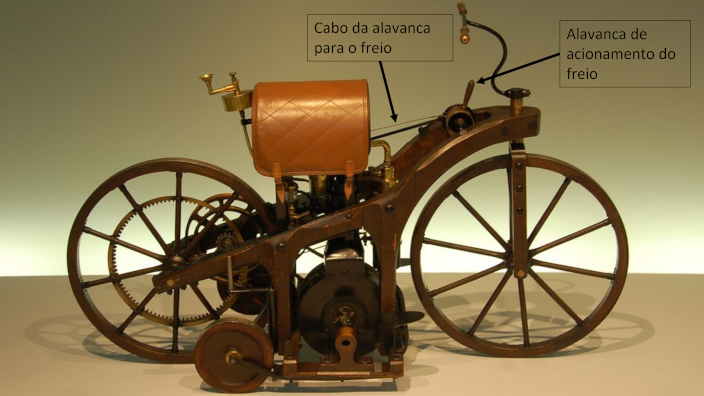
\includegraphics[width=8cm]{figuras/primeira-motocicleta-0.5cv-velocidade-maxima-12kmh.PNG}}
    }{
        \Fonte{\href{https://en.wikipedia.org/wiki/Daimler_Reitwagen}{wikipedia.org}}
    }	
\end{figure}

Outra aparição um ano depois, foi na carruagem Daimler Figura~\ref{fig:Carruagem-Daimler}, com motores de combustão interna
1,1 cv e velocidade máxima de 16 km/h, o freio de sapata era instalado na frente das rodas traseiras e era acionado pisando no mesmo.

\begin{figure}[h!]
    \centering
    \Caption{\label{fig:Carruagem-Daimler} Carruagem Daimler 1886 }	
    \UNIFORfig{}{
        {\includegraphics[width=8cm]{figuras/carruagem-daimler-1886.png}}
    }{
        \Fonte{\href{https://pin.it/2lkAp6m}{Pinterest}}
    }	
\end{figure}

\subsection{Freios de banda e sapatas externas }

À medida que os pneus de borracha sólida rapidamente se estabeleceram para veículos motorizados (começando com o automóvel triangular Benz em 1886 e o carro com rodas de aço Daimler de 1889) e logo foram substituídos por pneus de borracha cheios de ar para um conforto mais confortável. passeio, a era do freio de sapata nos automóveis já havia chegado ao fim. 

A partir de então, começaram a ser utilizados freios de banda (faixas de freio de aço flexíveis que freavam diretamente ou por meio de diversas sapatas de freio rebitadas por dentro) ou freios de sapata externos (ferro fundido rígido ou sapatas de freio de aço com lonas de freio). Esses freios acionados por pedal funcionavam com tambores de freio externos que normalmente eram instalados na frente, no eixo de transmissão intermediário ou no eixo de transmissão, na área da roda traseira. Por exemplo, a Fahrzeugfabrik Eisenach produziu o primeiro automóvel Wartburg em 1898. O Modelo 1 apresentava uma transmissão exposta e pinhões de transmissão. Os freios de banda frearam tanto o eixo quanto as duas rodas traseiras. 

Em 1899, o carro com rodas de aço da Daimler tinha pneus de borracha maciça e freios de banda de aço nas rodas traseiras (Fig. 4). O Daimler “Phoenix”, também datado de 1899, ainda tinha pneus de borracha maciça, mas estes foram logo substituídos por pneus cheios de ar. Um freio de pé atuou como freio de sapata externo no eixo de transmissão dianteiro (Figuras 5 e 6), e o freio de mão atuou nas rodas traseiras. Além disso, este carro apresentava – tal como, por exemplo, o carro de corrida Benz de 1899 (Fig. 7) – um “freio sprag”, uma haste forte montada na parte traseira que tinha a finalidade de ser conduzida contra o (normalmente relativamente). estrada suave). 

Um trecho do texto original do manual do usuário do “Phaeton” de Benz \& Co. Rheinische Gasmotoren-Fabrik AG Mannheim de 1902 diz o seguinte: “Além de um freio de mão preso no lado esquerdo, o carro é freado principalmente por pressionando o pedal esquerdo, que funciona como freio de banda nos discos de freio fixados nas duas rodas traseiras. Simultaneamente, como mencionado acima, a correia é automaticamente movida para fora. Para parar o carro imediatamente, os pedais esquerdo e direito são pressionados ao mesmo tempo, o que faz com que o freio de fita conectado ao pedal direito atue sobre o disco de freio e freie a caixa de redução.”

\subsection{Freios a tambor de sapata interna com acionamento mecânico por cabo} 

Com o tempo, os veículos tornaram-se mais rápidos e pesados. Portanto, eles precisavam de um sistema de freio mais eficaz. Assim, os freios de banda e de sapata externa logo deram lugar ao freio de tambor de sapata interno, para o qual Louis Renault solicitou uma patente em 1902. Um mecanismo de espalhamento empurrava duas sapatas de freio em forma de crescente contra a superfície interna do freio de ferro fundido ou aço. tambores, que estavam conectados à roda. Devido ao seu efeito de auto-reforço, o freio a tambor apresenta forças operacionais baixas em comparação com as forças de frenagem, longos períodos de manutenção e lonas de longa duração. 

Inicialmente, a força de frenagem era transmitida aos dois freios a tambor das rodas traseiras por meio de cabos de freio. 

Por exemplo, o Mercedes Simplex já apresentava freios a tambor adicionais nas rodas traseiras operados por cabo (Fig. 8), além do freio de banda do eixo cardan. Devido ao maior desempenho do motor (40 cavalos de potência), foi adicionado um segundo freio de pé (Fig. 9), que também atuou como freio de faixa no eixo intermediário da transmissão por corrente. A propósito, todos os quatro freios eram resfriados por um jato de água que, durante a frenagem, pingava de um reservatório nas superfícies de atrito. 

A partir de cerca de 1920, os veículos foram equipados com freios a tambor nas quatro rodas. A força de frenagem ainda era transmitida por meios mecânicos, ou seja, alavancas, juntas e cabos de freio.
    
Esses freios a tambor operados por cabo permaneceram em uso por muito tempo. Um exemplo foi o modelo padrão da VW da década de 1950 (Fig. 10): 

O elemento principal deste sistema de freio era um trilho de pressão do freio (Item 1). Os quatro cabos de freio (2) fixados a este elemento corriam para trás através das mangas dos cabos até os freios das rodas (freios a tambor) das quatro rodas (3). A parte traseira do trilho era sustentada por uma alavanca curta que ficava no eixo do pedal do freio. Quando o pedal do freio (4) foi pressionado, o trilho de pressão do freio foi empurrado para frente com os quatro cabos. Os cabos transmitiram a força aos freios das rodas. 

A alavanca do freio de mão (5) ficava mais atrás no carro. Contudo, por meio de uma haste desacoplada, o freio de mão atuava, em última análise, sobre o mesmo mecanismo que o freio de pé e, portanto, atuava igualmente sobre as quatro rodas.
    
\subsection{Acionamento do freio hidráulico }

O principal problema do freio a cabo era o grande esforço de manutenção e o efeito de frenagem desigual causado pelo atrito desigual durante a transmissão mecânica. 

Isso foi remediado quando a Lockheed introduziu um freio acionado hidraulicamente em 1919. Um fluido de freio especial agora transmitia a força do pedal do freio uniformemente aos cilindros de atuação dos freios das rodas mediante linhas e mangueiras de metal, sem a necessidade de alavancas, juntas e freios. cabos. 

A ativação do freio hidráulico também possibilitou amplificar a pressão do pé aplicada pelo motorista usando a depressão do coletor de admissão como fonte de energia para um sistema servo de freio. O princípio foi patenteado em 1919 pela Hispano-Suiza. 

Em veículos comerciais e material circulante ferroviário, os freios pneumáticos estabeleceram-se como o sistema de escolha.

Em 1926, o “Adler Standard” foi o primeiro automóvel na Europa a ser equipado com um sistema de travagem hidráulico. O primeiro reforço hidráulico da força de travagem nas corridas de automóveis foi utilizado no Mercedes-Benz “Silver Arrows” em 1954. Este acabou por se tornar equipamento padrão para muitos veículos de produção em massa. 

Como uma possível falha do circuito de freio poderia desabilitar completamente os primeiros freios de circuito único, o freio de circuito duplo foi posteriormente prescrito por lei. Conforme o desenvolvedor do VW Golf, Dr. Ernst Fiala, os primeiros “Beetles” (o modelo padrão dos VWs) ainda tinham um freio acionado por cabo exatamente por esse motivo: na época, temia-se que uma mangueira nos freios hidráulicos pudesse explodir. Mais tarde, porém – mesmo que apenas por razões competitivas – o \textit{VW Export} e o \textit{VW Transporter} apresentavam sistemas de travagem hidráulicos.

\subsection{Freio a disco }

Embora a montadora britânica Lancaster tenha patenteado o freio a disco em 1902, demorou muito até que esse tipo de freio fosse introduzido. Só cerca de cinquenta anos mais tarde, a partir de 1955, é que o lendário Citroën DS-19 se tornou o primeiro automóvel produzido em massa a ser equipado com freios de disco. O freio a disco foi derivado do freio multi-disco e foi desenvolvido inicialmente para a indústria aeronáutica. 

No freio a disco, uma lona de freio pressiona o disco de freio por dentro e por fora. O disco de freio (normalmente feito de ferro fundido ou, menos comumente, de aço) é conectado à roda. Sua vantagem é a estrutura simples e de fácil montagem. Também neutraliza a redução do efeito de travagem causado pelo sobreaquecimento e evita o desalinhamento das rodas de um eixo. 

O primeiro carro alemão com freios a disco nas rodas dianteiras foi o BMW 502 em 1959. Os primeiros carros alemães a ter freios a disco nas quatro rodas foram o Mercedes 300 SE, o Lancia Flavia e o Fiat 2300 em 1961. Hoje, praticamente todos os carros possuem sistema de freio a disco, pelo menos nas rodas dianteiras. Em 1974, foram introduzidos os primeiros carros de corrida de Fórmula 1 com discos de freio compostos de fibra de carbono. Esses discos são considerados especialmente leves e resistentes ao calor e, portanto, ganharam amplo uso no automobilismo e na aviação.

\subsection{Pastilhas e sapatas de freio} 

Foi necessário desenvolver lonas de freio adequadas para freios a tambor e a disco, para os quais o amianto provou ser particularmente eficaz. Só quando se soube que as fibras de amianto eram prejudiciais à saúde é que o material foi substituído pela fibra plástica.

\subsection{Sistemas de estabilidade de condução }

A era dos sistemas de travagem eletrônicos começou em 1978 com a chegada do sistema de travagem anti bloqueio (ABS) para automóveis desenvolvidos pela Bosch. Durante a frenagem, o ABS fornece detecção precoce do travamento incipiente de uma ou mais rodas e evita o travamento das rodas. Garante a dirigibilidade do veículo e reduz substancialmente o perigo de derrapagem. Em 1986, foi seguido pelo sistema de controlo de tração (TCS), com o qual a Bosch alargou a capacidade do sistema para o controlo da patinagem das rodas sob aceleração. A Fig. 11 mostra testes de estrada destes sistemas no campo de testes da Bosch em Boxberg, no sul da Alemanha.

Como uma melhoria adicional na segurança de condução, a Bosch introduziu o programa eletrônico de estabilidade (ESP) em 1995, que integra as funções do ABS e do TCS. Ele não apenas evita que as rodas do veículo travem e girem, mas também evita que o veículo puxe para o lado. Sistemas alternativos, como a direção nas quatro rodas e a cinemática do eixo traseiro, desenvolvidos nas décadas de 1980 e 1990 e foram instalados em alguns veículos de produção em massa, não se popularizaram porque pesavam muito e custavam muito caro. ou não foram suficientemente eficazes.

Enquanto isso, o controle de freio \textit{sen sotronic} (eletro-hidráulico) encontrou seu lugar na construção de automóveis. Fornece todas as funções do ESP e desacopla o funcionamento mecânico do pedal do freio por meio de um sistema de controlo eletrônico. Por motivos de segurança, um sistema hidráulico de reserva está automaticamente disponível.

\section{Classificação dos sistemas de travagem dos automóveis}

Todos os sistemas de frenagem de um veículo são chamados de equipamentos de frenagem. Os sistemas de freio dos automóveis podem ser classificados com base em

\begin{itemize}
    \item design e
    \item método de operação
\end{itemize}

\subsection{Designs}

Com base nos requisitos legais, as funções do equipamento de travagem são partilhadas entre três sistemas de travagem:

\begin{itemize}
    \item os freios de serviço,
    \item o sistema de freio secundário, e
    \item o freio de estacionamento
\end{itemize}

Nos veículos comerciais, o equipamento de travagem também inclui um sistema de travagem de funcionamento contínuo (por exemplo, retardador) que permite ao condutor manter o veículo a uma velocidade constante numa descida longa. O equipamento de travagem de um veículo comercial inclui também um sistema de travagem automático que acciona os freios de um reboque se este for desengatado do veículo trator, deliberadamente ou por acidente.

\subsection{Freios de serviço}

O sistema de freio de serviço (“freio de pé”) é utilizado para desacelerar o veículo, manter sua velocidade constante em uma descida ou pará-lo completamente. 

O condutor pode variar infinitamente o efeito de travagem através da pressão aplicada no pedal do travão. O sistema de freio de serviço aciona os freios nas quatro rodas.

\subsection{Sistema de freio secundário }

O sistema de freio secundário deve ser capaz de fornecer pelo menos algum grau de frenagem caso o sistema de freio de serviço falhe. Deve ser possível variar infinitamente o nível de travagem aplicado. 

O sistema de freio secundário não precisa ser um terceiro sistema de freio totalmente separado (além dos freios de serviço e do freio de estacionamento) com seu próprio dispositivo de atuação separado. Pode consistir no circuito intacto restante de um sistema de freio de serviço de circuito duplo no qual um circuito falhou, ou pode ser um freio de estacionamento capaz de aplicação gradual.


\subsection{Sistema de freio de estacionamento }

O freio de estacionamento (freio de mão) desempenha a terceira função exigida do equipamento de freio. Deve impedir que o veículo se mova quando parado ou estacionado, mesmo em declive e quando o veículo estiver desacompanhado. 

Conforme os requisitos legais, o sistema de freio de estacionamento também deve ter uma ligação mecânica intacta, por ex. uma ligação de haste ou cabo, entre o dispositivo de atuação e os freios que ele opera. 

O sistema de freio de estacionamento é geralmente accionado por meio de uma alavanca do freio de mão posicionada perto do banco do condutor ou, em alguns casos, por um pedal. Isto significa que os sistemas de freio de serviço e de estacionamento de um veículo motorizado possuem dispositivos de atuação e meios de transmissão de força separados. 

O sistema de freio de estacionamento é capaz de aplicação gradual e aciona os freios apenas em um par de rodas (dianteiras ou traseiras)


\section{Métodos de operação}

Dependendo de serem operados total ou parcialmente pelo esforço humano, ou por outra fonte de energia, os sistemas de travagem podem ser classificados como

\begin{itemize}
    \item sistemas de frenagem de energia muscular (não assistida),
    \item sistemas de travagem assistidos, ou
    \item sistemas de freio elétrico,
\end{itemize}

\subsection{Sistemas de frenagem de energia muscular }

Neste tipo de sistema de frenagem, frequentemente encontrado em carros e motocicletas, o esforço aplicado ao pedal do freio ou à alavanca do freio de mão é transmitido aos freios de forma mecânica (por meio de uma haste ou cabo) ou hidraulicamente. A energia pela qual a força de travagem é gerada é produzida inteiramente pela força física do condutor.

\subsection{Sistemas de travagem assistida }

O sistema de travagem assistida é o tipo mais comumente utilizado em automóveis e veículos comerciais ligeiros. Amplifica a força aplicada pelo motorista por meio de um servofreio que utiliza outra fonte de energia (vácuo ou hidráulica). A potência muscular amplificada é transmitida hidraulicamente aos freios.

\subsection{Sistemas de freios elétricos }

Os sistemas de freios elétricos são geralmente usados em veículos comerciais, mas são ocasionalmente instalados em carros grandes em conjunto com um sistema ABS integral. Este tipo de sistema de travagem é operado inteiramente sem energia muscular.

O sistema é operado por energia hidráulica (que se baseia na pressão do fluido) transmitida por meios hidráulicos. O fluido de freio é armazenado em acumuladores de energia (acumuladores hidráulicos) que também contêm um gás comprimido (geralmente nitrogênio). O gás e o fluido são mantidos separados por um diafragma flexível (acumulador de diafragma) ou um pistão com vedação de borracha (acumulador de pistão). Uma bomba hidráulica gera a pressão do fluido, que está sempre em equilíbrio com a pressão do gás no acumulador de energia. Um regulador de pressão coloca a bomba hidráulica em marcha lenta assim que a pressão máxima é atingida.

Como o fluido de freio pode ser considerado praticamente incompressível, pequenos volumes de fluido de freio podem transmitir grandes pressões ao sistema de freio.



% !TeX root = ../documento.tex
\chapter{O Estado da Arte}
\label{cap:o-estado-da-arte}

Este capítulo apresenta uma análise histórica e técnica do componente alvo desta pesquisa, o sistema de freio. São explorados os principais marcos e inovações tecnológicas, bem como os diferentes tipos de freios e sua evolução mecânica e elétrica. São descritos os componentes e seus princípios de funcionamento, além de serem discutidos estudos experimentais e teóricos, desafios, limitações e tendências de aplicação. O objetivo é fornecer subsídios para a compreensão do contexto atual e identificar oportunidades para futuras contribuições acadêmicas.


\section{Histórico dos Sistemas de Freio}
\label{sec:o-estado-da-arte-1}


\subsection{Evolução dos Sistemas de Freio ao Longo do Tempo}
\label{sec:o-estado-da-arte-1-1}
Os sistemas de freio passaram por diversas etapas de desenvolvimento, desde métodos rudimentares utilizados em carruagens na antiguidade até sistemas eletrônicos modernos e freios regenerativos. A literatura destaca que essas transformações ocorreram de forma gradual, acompanhando avanços tecnológicos e demandas de segurança veicular.


\subsection{Principais Marcos e Inovações Tecnológicas}
\label{sec:o-estado-da-arte-1-2}
Inicialmente, os freios eram simples, como o uso de varas de madeira contra as rodas. Em 1850, foi introduzido o freio de sapata em carruagens REIF (2014). No século XVIII, o uso de freios de fricção entre um rotor e um estator foi introduzido em carruagens puxadas por cavalos e, posteriormente, adaptado para veículos automotivos no final do século XIX BRYANT (2022). A patente do freio a disco ocorreu em 1902 por George Westinghouse, embora sua adoção em massa tenha ocorrido apenas na década de 1950 \cite{Konrad2014}.

A introdução do sistema hidráulico na década de 1920, pelo engenheiro americano Tom Reilly, permitiu uma distribuição mais uniforme da força de frenagem \cite{Lentin2022}, substituindo sistemas mecânicos (como cabos ou varas) por fluido. Os freios de tambor nas quatro rodas se popularizaram nesse período, evoluindo para freios a disco a partir de 1959 \cite{Konrad2014}. O desenvolvimento do \textit{Anti-lock Braking System} (ABS) na década de 1970, que revolucionou a segurança veicular, representou um avanço importante ao permitir o controle direcional durante a frenagem \cite{AndrewJ2022}.

A transição para sistemas de freio \textit{"by-wire"} (sem conexão mecânica direta) é destacada como um marco relevante a partir dos anos 1990 \cite{Donghai2022}. Entre os avanços recentes, destacam-se sistemas eletrônicos como Controle Eletrônico de Estabilidade (ESC), Distribuição Eletrônica de Frenagem (EBD), Sistema de Frenagem Autônoma de Emergência (AEB) \cite{Lentin2022}, sistemas de freio adaptativos e frenagem regenerativa.

Em suma, os sistemas de frenagem veicular têm experienciado um avanço tecnológico substancialmente acelerado, especialmente nas últimas décadas, superando o progresso acumulado ao longo de séculos anteriores.

Isso porque, enquanto os séculos XIX e XX foram marcados por evoluções mecânicas e hidráulicas lentas e graduais, o século XXI, promovido especialmente por inovações em eletrônica, inteligência artificial e interoperabilidade de sistemas, promoveu uma revolução qualitativa nos mecanismos de frenagem. A Figura~\ref{fig:trajetoria_historica_evolucao_tecnologia_adas} apresenta esta evolução em níveis.

Essa transformação se reverbera não apenas no avanço técnico, mas também em uma mudança de paradigma na função do sistema de frenagem, que passa a atuar como elemento ativo na prevenção de acidentes, melhora da segurança, além de contribuir para a conveniência e conforto na direção, conforme é demonstrado na Figura~\ref{fig:trajetoria_historica_evolucao_tecnologia_adas}.

\begin{figure}[htbp]
    \centering
    \caption{Trajetória da automação dos veículos nas últimas décadas.}
    \label{fig:trajetoria_historica_evolucao_tecnologia_adas}
    \fbox{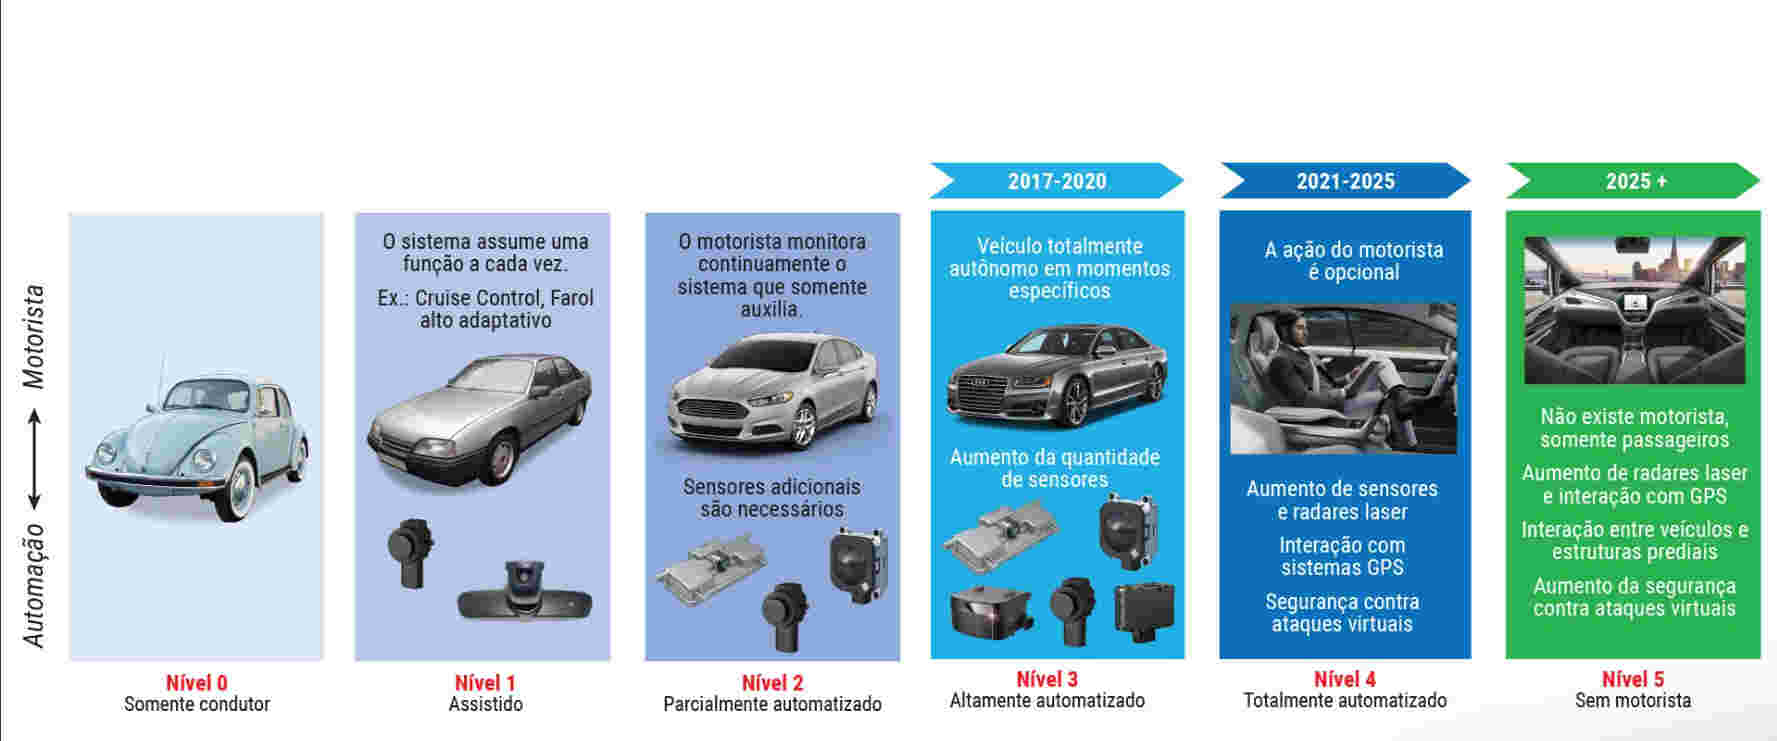
\includegraphics[width=0.8\textwidth]{figuras/trajetoria_historica_evolucao_tecnologia_adas.jpg}}
    \fonte{ O Autor, adaptado de \cite{evolucaodosistemaemniveis2022}. }
\end{figure}

\section{Classificação dos Sistemas de Freio}
\label{sec:o-estado-da-arte-1-3}
Os sistemas de freio podem ser classificados em várias categorias, segundo o princípio de funcionamento e aplicação. Conforme discutido por \citeonline{Konrad2014} e \citeonline{Lentin2022}, existem sistemas que geram atrito para reduzir a velocidade do veículo, como o freio a tambor, que utiliza sapatas que se expandem contra um tambor para gerar atrito, e o freio a disco, que utiliza pastilhas pressionando um disco rotativo \cite{Lentin2022}.

%Sistemas híbridos, que combinam freios a disco nas rodas dianteiras e freios a tambor nas rodas traseiras \cite{Lentin2022}, ainda são comuns em veículos econômicos devido ao custo-benefício. Essa configuração é frequentemente adotada por fabricantes para equilibrar eficiência, custo de produção e manutenção, além de considerar a distribuição de peso do veículo, já que a maioria do peso está na dianteira, onde os freios a disco são mais eficientes, enquanto os freios a tambor são adequados para a traseira, onde a frenagem é menos intensa.

Sistemas híbridos, que combinam freios a disco nas rodas dianteiras e freios a tambor nas rodas traseiras \cite{Lentin2022}, ainda são comuns em veículos econômicos devido ao custo-benefício. Essa configuração é frequentemente adotada por fabricantes por equilibrar desempenho e custo, uma vez que, durante a frenagem, ocorre a transferência dinâmica de carga para o eixo dianteiro, que demanda maior capacidade de dissipação térmica — característica típica dos freios a disco — enquanto o eixo traseiro está sujeito a menores esforços, sendo adequadamente atendido por freios a tambor \cite{Rudolf2011}.

Os sistemas de freio regenerativos, utilizados em veículos híbridos e elétricos, permitem a recuperação de energia durante a frenagem. Nesses sistemas, a energia gerada durante a frenagem é convertida em eletricidade e armazenada na bateria do veículo, promovendo maior eficiência energética e autonomia \cite{Donghai2022}. Estudos recentes publicados em periódicos como IEEE \textit{Transactions on Vehicular Technology} destacam o potencial desses sistemas para contribuir com a sustentabilidade e eficiência dos veículos elétricos, embora ressaltem desafios relacionados à integração com sistemas convencionais de frenagem e à validação em diferentes condições de operação \cite{Kumar2024}.

Além disso, alternativas modernas incluem sistemas eletro-hidráulicos, que utilizam controle eletrônico para regular a pressão hidráulica aplicada às pinças de freio, e sistemas eletromagnéticos, que interagem diretamente com o sistema de movimento do veículo, especialmente em aplicações de veículos autônomos \cite{Donghai2022}.

Ainda relacionado aos sistemas eletro-hidráulicos, estudos recentes também demonstram a relevância do projeto paramétrico de motores integrados a sistemas de freio eletro-hidráulicos em veículos elétricos, evidenciando ganhos em eficiência e resposta dinâmica \cite{MotorParametricDesign2023}. Adicionalmente, estratégias de controle coordenado de pressão têm sido propostas para aprimorar a precisão e robustez desses sistemas, conforme discutido em \citeonline{PressureCoordinatedControl2023}. A literatura técnica explora a potencial aplicação dessas alternativas, destacando a necessidade de análises experimentais e validações em ambientes reais para avaliar sua eficiência e confiabilidade.

Portanto, a classificação dos sistemas de freio apresentada neste capítulo busca contribuir para a compreensão das diferentes tecnologias disponíveis e, possíveis soluções que podem ser exploradas em contextos acadêmicos e industriais. A análise das configurações e princípios de funcionamento dos sistemas de freio é fundamental para validar modelos matemáticos e estratégias de controle, bem como para identificar limitações e oportunidades de investigação na área de sistemas automotivos.


\section{Tipos de Sistemas de Freio}
\label{sec:o-estado-da-arte-2}


\subsection{Freios a disco e a tambor}
\label{sec:o-estado-da-arte-2-1}
Os freios a disco e a tambor são os dois principais tipos de sistemas de freio utilizados em veículos. Os freios a disco (Figura~\ref{fig:freio-disco}) são conhecidos por sua eficiência na dissipação de calor, durabilidade e desempenho consistente em diferentes condições de operação. São amplamente utilizados em veículos modernos, especialmente nas rodas dianteiras e, cada vez mais, nas traseiras \cite{Konrad2014}. Eles utilizam pastilhas que são pressionadas contra um disco rotativo, proporcionando desempenho de frenagem adequado em altas velocidades \cite{AndrewJ2022}.

\begin{figure}[htbp]
    \centering
    \caption{Freio a Disco.}
    \label{fig:freio-disco}
    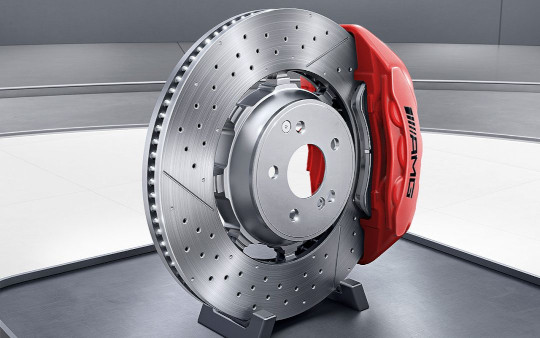
\includegraphics[width=0.8\textwidth]{figuras/freio-disco.jpg}
    \fonte{ O Autor, adaptado de \cite{freioadisco2023}. }
\end{figure}

A literatura técnica apresenta diversas análises sobre o desempenho térmico e desgaste dos freios a disco, destacando sua potencial aplicação em veículos de passeio e comerciais \cite{Reboucas2025}. Estudos experimentais e simulações computacionais têm contribuído para a validação de modelos matemáticos que descrevem o comportamento desses sistemas sob diferentes condições de carga e temperatura \cite{ChenQuguang2019}. Tais contribuições oferecem subsídios para futuras pesquisas voltadas à otimização de materiais de fricção e ao desenvolvimento de estratégias de controle para sistemas de freio.

Por outro lado, os freios a tambor (Figura~\ref{fig:freio-tambor}) utilizam sapatas com revestimento de material de fricção (abrasivo), que se expandem contra a superfície interna de um tambor. Estes sistemas são mais econômicos e ainda comuns em veículos menores e de baixo custo \cite{Konrad2014}. A análise de sua eficiência e durabilidade é tema recorrente em estudos acadêmicos, que também exploram suas limitações, especialmente relacionadas à dissipação de calor e ao desgaste dos componentes \cite{Reboucas2025}.

\begin{figure}[htbp]
    \centering
    \caption{Freio a Tambor.}
    \label{fig:freio-tambor}
    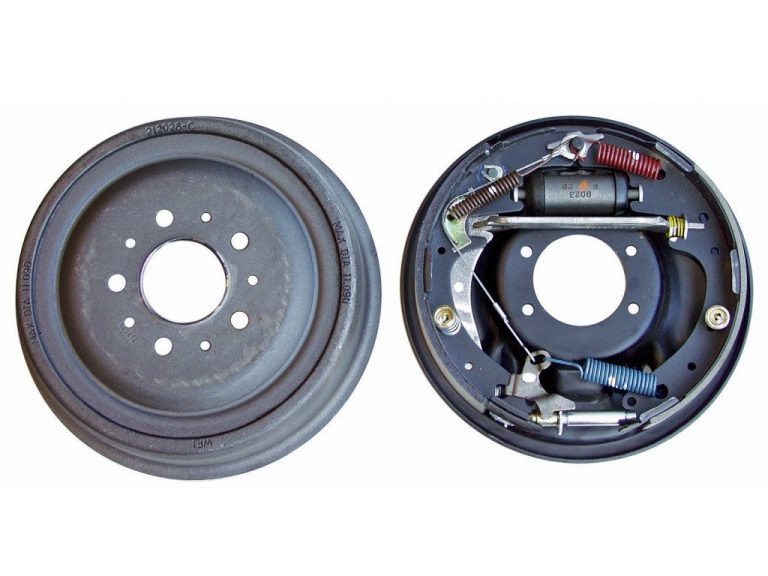
\includegraphics[width=0.8\textwidth]{figuras/freio-tambor.jpg}
    \fonte{ O Autor, adaptado de \cite{freioATambor}. }
\end{figure}

A escolha entre freios a disco e a tambor depende de fatores como custo, distribuição de peso do veículo, intensidade da frenagem exigida e requisitos de manutenção. A literatura sugere que sistemas híbridos, combinando ambos os tipos, podem ser uma alternativa viável para determinadas aplicações, especialmente em veículos econômicos \cite{AmbeMohammedHussein2024}.

Essas análises e explorações favorecem o entendimento das potencialidades e limitações dos sistemas de freio, oferecendo contribuições para a validação de modelos e desenvolvimento de novas soluções na área automotiva.


\subsection{Sistemas de Freio Hidráulico e Pneumático}
\label{sec:o-estado-da-arte-2-2}
Os sistemas de freio podem ser classificados em hidráulicos e pneumáticos. Os sistemas hidráulicos. Figura~\ref{fig:sistemas_hidraulicos}, que utilizam fluido de freio para transmitir a força do pedal aos freios, são os mais comuns em veículos leves \cite{Konrad2014, AndrewJ2022}. Esses sistemas incluem componentes como cilindros mestres, válvulas de controle de pressão e sistemas de reforço (\textit{boosters}) \cite{Rudolf2011}.

\begin{figure}[htbp]
    \centering
    \caption{Sistemas Hidráulicos.}
    \label{fig:sistemas_hidraulicos}
    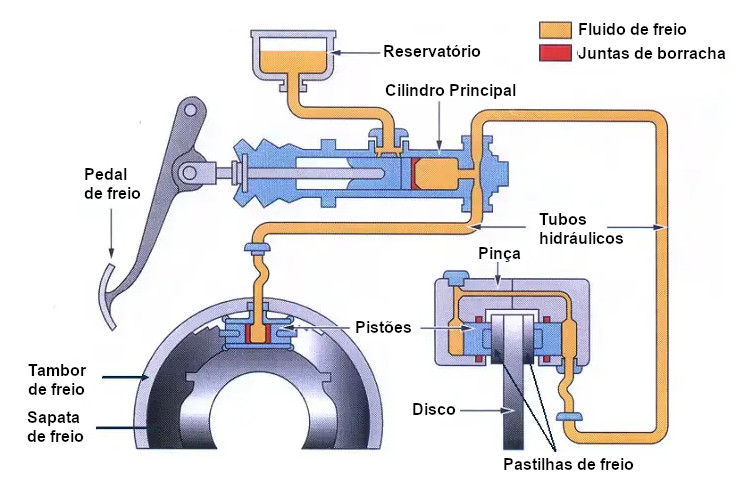
\includegraphics[width=0.8\textwidth]{figuras/sistemas_hidraulicos.jpg}
    \fonte{ O Autor, adaptado de \cite{sistemahidraulico}. }
\end{figure}

Já os sistemas pneumáticos. Figura~\ref{fig:sistemas_pneumatico}, que utilizam ar comprimido ou outro gás pressurizado para aplicar a força de frenagem, são predominantes em veículos pesados, como caminhões e ônibus \cite{Konrad2014}. De acordo com análises recentes, esses sistemas apresentam potencial aplicação em veículos de grande porte devido à sua capacidade de gerar força suficiente para frear veículos com grande massa, além de serem reconhecidos por sua durabilidade e segurança operacional \cite{BuHanShue2007}.

\begin{figure}[htbp]
    \centering
    \caption{Sistemas Pneumáticos.}
    \label{fig:sistemas_pneumatico}
    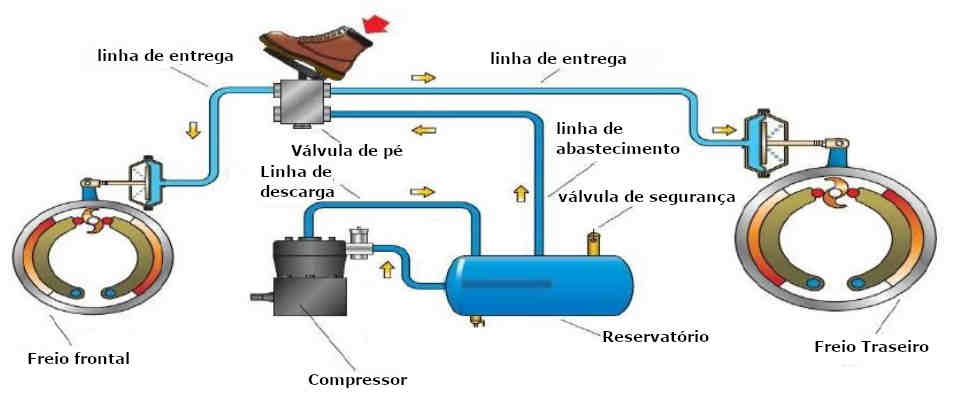
\includegraphics[width=0.8\textwidth]{figuras/sistemas_pneumatico.jpg}
    \fonte{ O Autor, adaptado de \cite{sistemapneumaticos}. }
\end{figure}

\subsection{Tecnologias Modernas}
\label{sec:o-estado-da-arte-2-3}
As tecnologias modernas têm contribuído para avanços na segurança, eficiência e desempenho dos veículos \cite{Konrad2014}. A capacidade dos sistemas de freio de fornecer desaceleração controlada e estável, mesmo em condições adversas, tem sido examinado e corroborado por inúmeras investigações acadêmicas \cite{AndrewJ2022}.

O ABS (\textit{Anti-lock Braking System}), por exemplo, evita o travamento das rodas durante a frenagem \cite{Donghai2022}, sendo considerada uma das tecnologias mais amplamente utilizadas em veículos modernos. Estudos recentes exploram o potencial do ABS para melhorar o controle do veículo e reduzir o risco de derrapagem, especialmente em pisos escorregadios \cite{Rajkumar2024}. A modulação da pressão de frenagem permite que o motorista mantenha o controle do veículo durante frenagens de emergência, sendo uma contribuição relevante para a segurança veicular \cite{Rajkumar2024}.

O ABS possui papel indispensável na segurança ao preservar a dirigibilidade e o controle direcional do veículo durante frenagens intensas, reduzindo o risco de derrapagem por travamento. Em algumas condições de baixa aderência e/ou superfícies soltas, a distância de frenagem pode não ser minimizada em relação ao bloqueio total, mas o benefício principal do ABS permanece associado à estabilidade e capacidade de manobra \cite{Rudolf2011, Lentin2022}.

Além do uso clássico em frenagem comandada pelo condutor, a mesma infraestrutura eletro-hidráulica de unidades ABS/ESC é empregada por funções como ESC e aplicações ADAS (por exemplo, ACC/AEB) para realizar intervenções de \textbf{frenagem ativa}, impondo perfis de pressão por roda a partir de referências geradas eletronicamente.
Além do ABS, outras tecnologias complementares têm sido amplamente exploradas e validadas, tais como:

\begin{itemize}
    \item \textbf{ESC (Controle Eletrônico de Estabilidade):} O ESC corrige a trajetória do veículo em situações de derrapagem como indicado na Figura~\ref{fig:controle_eletronico_estabilidade}, integrando-se ao ABS para fornecer um controle preciso da força de frenagem \cite{Konrad2014, Lentin2022}. Estudos destacam o potencial do ESC para contribuir com a estabilidade veicular em situações críticas \cite{Donghai2022}.

          \begin{figure}[htbp]
              \centering
              \caption{Controle Eletrônico de Estabilidade (ESC).}
              \label{fig:controle_eletronico_estabilidade}
              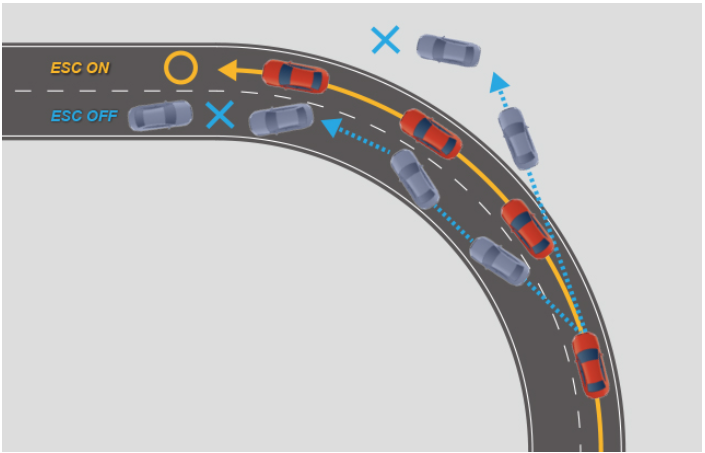
\includegraphics[width=0.8\textwidth]{figuras/controle_eletronico_estabilidade.jpg}
              \fonte{ O Autor, adaptado de \cite{controleeletronicodeestabilidadeESC}. }
          \end{figure}

    \item \textbf{EBD (Distribuição Eletrônica de Frenagem):} O EBD distribui a força de frenagem de forma equilibrada entre os eixos, melhorando a estabilidade do veículo \cite{Konrad2014}. Esse sistema é especialmente útil em veículos com carga variável, garantindo uma frenagem eficiente em todas as condições \cite{Rudolf2011}.

    \item \textbf{BAS (Assistência de Frenagem):} O BAS aumenta a pressão de frenagem durante emergências, mesmo que o motorista não aplique força suficiente no pedal, garantindo uma frenagem eficaz e segura \cite{Donghai2022}.

    \item \textbf{TCS (Sistema de Controle de Tração):} O TCS evita a derrapagem das rodas motrizes ao reduzir o torque do motor ou aplicar os freios, melhorando a tração e a estabilidade do veículo em superfícies escorregadias \cite{Donghai2022}, Figura~\ref{fig:sistema_controle_tracao}. Em outras palavras, controla o deslizamento das rodas durante a aceleração \cite{Konrad2014, Lentin2022}.

          \begin{figure}[htbp]
              \centering
              \caption{Demostração da roda sem (TCS).}
              \label{fig:sistema_controle_tracao}
              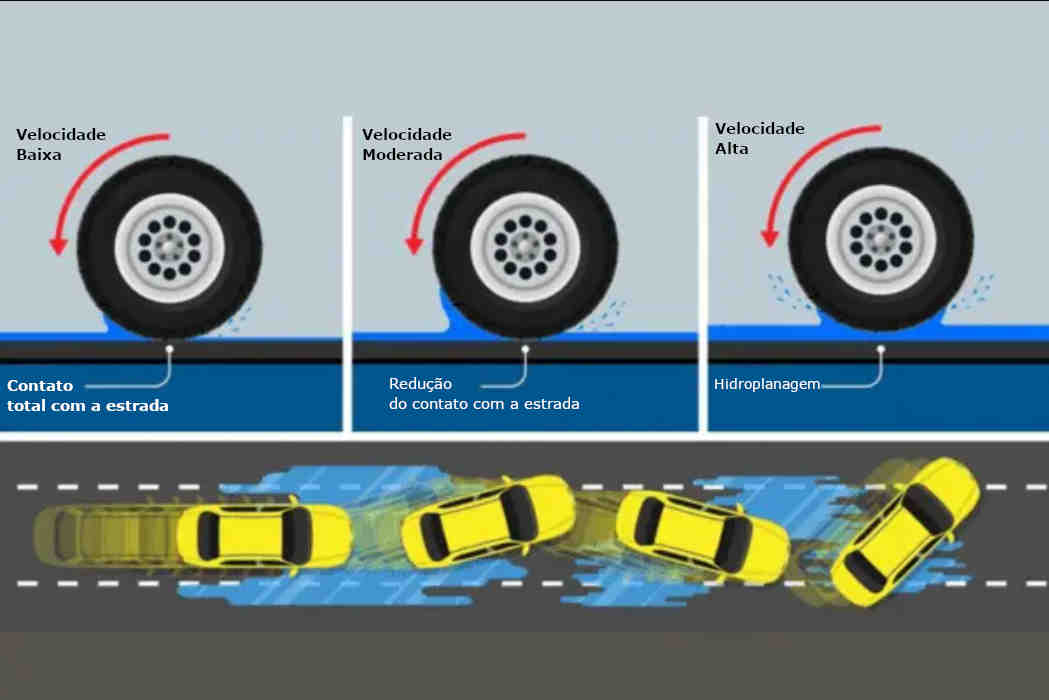
\includegraphics[width=0.8\textwidth]{figuras/sistema_controle_tracao.jpg}
              \fonte{ O Autor, adaptado de \cite{demostracaodarodasemTCS}. }
          \end{figure}

    \item \textbf{ACC (Controle de Cruzeiro Adaptativo):}  ajusta automaticamente a velocidade do veículo com base no tráfego à frente, mantendo uma distância segura em relação ao veículo precedente \cite{Konrad2014, Rudolf2011, Lentin2022}. Para isso, o sistema utiliza predominantemente sensores de radar instalados na parte frontal do veículo, capazes de medir continuamente a distância e a velocidade relativa dos veículos à frente, permitindo a adaptação dinâmica da velocidade de cruzeiro, conforme ilustrado na Figura~\ref{fig:acc-controle-de-cruzeiro-adaptativo}.

          \begin{figure}[htbp]
              \centering
              \caption{Controle de Cruzeiro Adaptativo (ACC).}
              \label{fig:acc-controle-de-cruzeiro-adaptativo}
              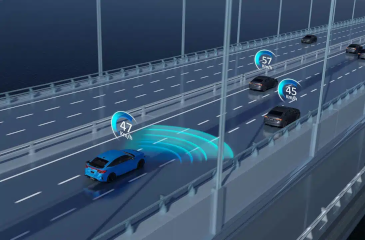
\includegraphics[width=0.8\textwidth]{figuras/acc-controle-de-cruzeiro-adaptativo.png}
              \fonte{ O Autor, adaptado de \cite{acc-controle-cruzeiro-adaptativo}. }
          \end{figure}

          Tendo em vista esses diferentes sistemas, o ADAS (Sistemas Avançados de Assistência ao Motorista) constitui um conjunto de tecnologias de assistência que pode integrar diversos desses recursos e empregar sensores, câmeras e outros dispositivos eletrônicos a fim de aumentar a segurança veicular e melhorar a experiência de condução. \cite{Konrad2014}


\end{itemize}

\section{Componentes dos Sistemas de Freio}
\label{sec:o-estado-da-arte-2-4}
Os sistemas de freio automotivo são compostos por diversos elementos, cuja configuração depende do tipo de tecnologia empregada. Nos sistemas de freio a disco e a tambor, destacam-se discos, tambores, pastilhas, sapatas e lonas, cada um desempenhando funções específicas na geração do atrito necessário para desacelerar o veículo. Sistemas hidráulicos incorporam cilindros mestres, válvulas de controle de pressão e servofreios, enquanto sistemas pneumáticos utilizam compressores de ar, válvulas e câmaras de freio \cite{Rudolf2011, Konrad2014, Lentin2022, AndrewJ2022}.

A presença de sensores, como os de velocidade das rodas, pressão e temperatura, é fundamental para o funcionamento de sistemas eletrônicos de frenagem, como ABS, ESC e ADAS. Esses sensores monitoram parâmetros críticos e permitem a atuação precisa dos sistemas de controle, contribuindo para a análise do desempenho em diferentes condições operacionais \cite{Konrad2014, Lentin2022}. Atuadores eletrônicos, como motores elétricos e mecanismos piezoelétricos, têm sido explorados em aplicações de freio \textit{“by-wire”} e freio eletrônico de estacionamento (EPB), ampliando as possibilidades de integração com sistemas avançados de assistência ao motorista \cite{HouhuaJingShihao2023}.

Além dos componentes tradicionais, a literatura discute o uso de materiais alternativos, como discos de cerâmica e carbono, que apresentam potencial para melhorar a dissipação de calor e a resistência ao desgaste, embora seu emprego ainda seja restrito por questões de custo e disponibilidade \cite{Lentin2022}. A escolha dos materiais de fricção, bem como o desenvolvimento de sensores e atuadores mais eficientes, permanece como tema de investigação, oferecendo oportunidades para reconhecimento de novos modelos e estratégias de controle.

\subsection{Descrição, Função e Importância dos principais componentes }
\label{sec:o-estado-da-arte-3-1}
Os principais componentes dos sistemas de freio desempenham funções essenciais para a segurança e eficiência do veículo:

\begin{itemize}
    \item \textbf{Discos e tambores:} Os discos de freio, geralmente feitos de ferro fundido ou aço, possuem variações ventiladas para melhor dissipação de calor \cite{Konrad2014}. Já os tambores de freio são compostos por sapatas e lonas que pressionam a superfície interna do tambor para gerar atrito \cite{Konrad2014}.
          Discos de cerâmica também são utilizados devido à sua capacidade de dissipação rápida de calor \cite{Lentin2022}.

          São responsáveis por dissipar a energia cinética do veículo, transformando-a em calor. A eficiência térmica e a resistência ao desgaste são fundamentais para garantir a segurança e a durabilidade do sistema de freio \cite{Rudolf2011, AndrewJ2022}.

    \item \textbf{Pastilhas e lonas:} As pastilhas de freio são feitas de materiais que oferecem alta resistência ao desgaste e ao calor, aplicando pressão nos discos para gerar atrito \cite{Konrad2014, Lentin2022}. As lonas de freio, utilizadas em sistemas de freio a tambor, possuem composições semelhantes às pastilhas e aplicam pressão nos tambores para gerar atrito \cite{Konrad2014, Lentin2022}.
          De modo que, a partir desse atrito, geram a força de frenagem necessária para parar o veículo. A escolha de materiais de fricção adequados é essencial para garantir alta resistência ao desgaste e ao calor \cite{Konrad2014, AndrewJ2022}.

    \item \textbf{Cilindros mestres e servofreios:} O cilindro mestre converte a força do pedal em pressão na linha hidráulica, distribuindo-a para os freios \cite{Konrad2014, Lentin2022}. O servofreio amplifica a força aplicada pelo motorista, utilizando vácuo do motor ou pressão hidráulica \cite{Konrad2014}. Garantindo que a força aplicada no pedal seja transmitida de forma eficiente para os freios, convertendo a força mecânica em pressão na linha do sistema hidráulico \cite{Konrad2014,Lentin2022}.

    \item \textbf{Sensores:} Sensores de velocidade das rodas são essenciais para sistemas como ABS e TCS, monitorando exclusivamente a velocidade das rodas \cite{Konrad2014, Lentin2022, AndrewJ2022}. Já a pressão do fluido de freio é monitorada por sensores de pressão específicos instalados no circuito hidráulico. Sensores de temperatura também auxiliam na análise do desempenho do sistema \cite{Konrad2014}. Esses sinais asseguram o funcionamento correto dos sistemas eletrônicos de frenagem, como ABS e ESC \cite{Konrad2014, AndrewJ2022}.

\end{itemize}


\subsection{Princípios de Funcionamento}
\label{sec:o-estado-da-arte-3-3}
Em suma, os sistemas de freio funcionam com base em princípios hidráulicos e mecânicos. Quando o pedal de freio é pressionado, a força aplicada pelo motorista é transmitida à haste do pedal e, em seguida, ao servofreio (quando presente), que amplifica essa força. Na sequência, o cilindro mestre converte essa força amplificada em pressão na linha hidráulica, que é então distribuída para os freios nas rodas por meio do circuito hidráulico \cite{Konrad2014, Lentin2022, Konrad2014}. Nos freios a disco, as pastilhas pressionam os discos, gerando atrito e dissipando energia cinética em forma de calor. Nos freios a tambor, as lonas pressionam a superfície interna dos tambores para gerar atrito de maneira similar \cite{Konrad2014, Lentin2022}.

Por outro lado, os sensores de velocidade das rodas monitoram continuamente as condições de rotação das rodas, mas não ajustam a pressão. A interpretação desses sinais é realizada pela unidade de controle eletrônico, que então \textbf{modula a pressão e a força de frenagem} por meio das válvulas e da bomba do sistema, assegurando a atuação correta de sistemas como ABS e ESC \cite{Konrad2014, AndrewJ2022}.

\begin{comment}
Em suma, os sistemas de freio funcionam com base em princípios hidráulicos e mecânicos. Quando o pedal de freio é pressionado, o cilindro mestre converte essa força em pressão hidráulica, distribuída para os freios nas rodas. Nos freios a disco, as pastilhas pressionam os discos, gerando atrito e dissipando a energia cinética em forma de calor. Nos freios a tambor, as lonas pressionam a superfície interna dos tambores, gerando atrito de maneira similar \cite{Konrad2014, Lentin2022}.

Por outro lado, os sensores de velocidade das rodas monitoram continuamente o desempenho do sistema de freio, ajustando  a pressão e a força de frenagem conforme necessário para garantir a segurança e a eficiência do veículo \cite{Konrad2014, AndrewJ2022}.

% esta subsecao foi comentado por motivo de orientacao na revisao pela banca

\section{Mecanismos de ação dos diferentes tipos de freio}
\label{sec:o-estado-da-arte-4}
Os sistemas de freio são essenciais para a segurança dos veículos, convertendo energia cinética em calor através do atrito. Existem diferentes tipos de freios, cada um com seus mecanismos específicos de ação.

\begin{itemize}
    \item \textbf{Freios a Tambor:} Nos freios a tambor, as lonas são pressionadas contra a superfície interna do tambor, também gerando atrito \cite{Konrad2014, Lentin2022}. Embora menos eficientes que os freios a disco, são comuns em veículos mais antigos e em sistemas de freio de estacionamento \cite{AndrewJ2022}.


    \item \textbf{Freios a Disco:} Os freios a disco funcionam pela pressão hidráulica que move as pastilhas contra o disco, gerando atrito e desacelerando o veículo \cite{Konrad2014, Lentin2022}. Esse sistema é eficiente e oferece uma resposta rápida, sendo amplamente utilizado em veículos modernos \cite{Rudolf2011}.



    \item \textbf{Sistemas Eletro-Hidráulicos e Eletromagnéticos:} Os sistemas eletro-hidráulicos e eletromagnéticos utilizam a geração de torque de frenagem e a regulação de pressão para distribuir a força entre os eixos dianteiro e traseiro, garantindo uma frenagem equilibrada \cite{Donghai2022}.
\end{itemize}
\end{comment}

%################################################################
%################################################################
%################################################################
\section{Revisão de estudos experimentais e teóricos sobre a eficiência e desempenho dos sistemas de freio}
\label{sec:o-estado-da-arte-5}
Diversos estudos destacam a relevância dos sistemas de freio para a segurança veicular. Pesquisas indicam que a integração de tecnologias como ABS e ESC está associada à redução do risco de acidentes, especialmente em condições adversas \cite{Rudolf2011, Donghai2022}. O desenvolvimento de sistemas de freio mais eficientes e a implementação de novas tecnologias continuam sendo temas de interesse para a indústria automotiva \cite{AndrewJ2022}.

Entre as abordagens experimentais, são realizados testes de frenagem em diferentes superfícies, como seca, molhada e com gelo, além da análise do desgaste de componentes \cite{Konrad2014}. Estudos sobre materiais de atrito, como pastilhas e discos, buscam compreender fatores que influenciam a durabilidade e eficiência dos freios \cite{Lentin2022}. Outros trabalhos discutem a distribuição da força de frenagem e o controle de modos de frenagem, incluindo a comparação entre frenagem regenerativa e por atrito, especialmente em sistemas híbridos \cite{Donghai2022}.

Além disso, investigações sobre o impacto dos materiais de atrito no desempenho dos freios consideram aspectos como temperatura, desgaste e distribuição de pressão \cite{Rudolf2011}. Estudos recentes também destacam a importância de modelar a evolução do coeficiente de atrito das lonas de freio para aprimorar a estimação da pressão de frenagem, especialmente em situações onde a medição direta é limitada ou sujeita a incertezas \cite{ZhangWang2021}.

Adicionalmente, pesquisas sobre o projeto paramétrico de motores em sistemas de freio eletro-hidráulicos têm demonstrado avanços na integração entre controle eletrônico e desempenho dinâmico, especialmente em veículos elétricos \cite{MotorParametricDesign2023}. A geração de \gls{NVH} também é objeto de análise, com estudos avaliando o comportamento de diferentes compostos de fricção sob variadas condições de operação \cite{AndrewJ2022}.

Cabe mencionar que pesquisas recentes têm explorado a influência da eletrônica embarcada e dos sensores inteligentes na avaliação do desempenho dos sistemas de freio \cite{Lentin2022}, especialmente em aplicações que envolvem ADAS e condução autônoma. A validação experimental e computacional desses sistemas contribui para o entendimento das limitações e potencialidades das tecnologias atuais, oferecendo subsídios para futuras investigações e desenvolvimento de soluções mais seguras e eficientes.

%################################################################
%################################################################
%################################################################
\section{Análise de dados de testes em simulações de frenagem}
\label{sec:o-estado-da-arte-5-1}
A avaliação do desempenho dos sistemas de freio é realizada por meio de diferentes métodos experimentais e computacionais. Testes práticos em pistas de prova, como os realizados no centro de testes da Bosch em \textit{Boxberg} Alemanha, permitem observar o comportamento dos sistemas em situações reais, incluindo frenagens de emergência, descidas prolongadas e fadiga térmica \cite{Rudolf2011}. Tais experimentos possibilitam a análise da resposta dos sistemas ABS e ESC/ESP (\textit{Electronic Stability Control}/\textit{Electronic Stability Program}), que atuam de forma integrada para promover maior estabilidade e segurança.

Além dos ensaios em campo, simulações computacionais têm sido amplamente utilizadas para prever o desempenho dos freios sob variadas condições de uso \cite{Lentin2022}. Modelos matemáticos e simulações em dinamômetros auxiliam na compreensão dos efeitos da temperatura, velocidade e tipo de material de fricção sobre a eficiência de frenagem \cite{AndrewJ2022}.

A utilização de bancadas de teste, como HIL \textit{hardware-in-the-loop}, contribuem para a validação de sistemas híbridos e regenerativos, permitindo a exploração de diferentes cenários operacionais \cite{Donghai2022}. Estudos como o de \cite{Lv2014} demonstram a eficácia da simulação HIL para testar estratégias de modulação de pressão em sistemas de freio hidráulico integrados à frenagem regenerativa em veículos elétricos.

A análise dos dados obtidos em testes e simulações fornece subsídios para o desenvolvimento de estratégias de controle e identificação de limitações dos sistemas atuais. Diversas pesquisas têm explorado a influência de variáveis ambientais, como umidade e temperatura, na resposta dos sistemas de freio, destacando a importância da validação em condições reais de operação. A integração de sensores avançados e algoritmos inteligentes representa uma potencial aplicação para aprimorar o monitoramento e a atuação dos sistemas de frenagem, especialmente em veículos equipados com ADAS\cite{KapinskiJamesDeshmukh2016}.

%################################################################
%################################################################
%################################################################
\section{Desafios e Limitações dos Sistemas de Freio Modernos}
\label{sec:o-estado-da-arte-5-2}
A pesquisa e o desenvolvimento de sistemas de freio automotivos enfrentam diversos desafios técnicos e tecnológicos. Entre as principais dificuldades, destaca-se a necessidade de materiais de atrito que conciliem eficiência, durabilidade e custo acessível, considerando o contexto competitivo do setor \cite{AndrewJ2022}. O desempenho dos freios sob diferentes condições de uso demanda simulações avançadas e testes extensivos, que buscam validar modelos matemáticos e prever o comportamento dos sistemas em situações reais \cite{Lentin2022}.

A integração de sistemas de freio com tecnologias autônomas e híbridas apresenta obstáculos relacionados à precisão dos sensores e atuadores, bem como à interoperabilidade entre diferentes módulos eletrônicos \cite{Donghai2022, Lentin2022}. Questões como a dependência de sensores em ambientes adversos, a eficiência energética dos sistemas eletromagnéticos e a necessidade de materiais de fricção mais leves e resistentes continuam sendo objeto de análise e discussão na literatura técnica.

Além disso, o gerenciamento térmico e a dissipação de energia durante frenagens intensas representam áreas que demandam aprimoramentos contínuos. O desenvolvimento de estratégias para minimizar o desgaste irregular de componentes e a influência de variáveis ambientais, como umidade e temperatura, permanece como tema relevante para futuras investigações \cite{Konrad2014, Rudolf2011}.

Outro aspecto que merece atenção é a segurança cibernética dos sistemas de freio conectados, especialmente em veículos equipados com ADAS e funções autônomas. A proteção contra ataques e falhas de comunicação é fundamental para garantir a confiabilidade dos sistemas em cenários de mobilidade inteligente.

Em síntese, os desafios enfrentados pelos sistemas de freio modernos refletem a complexidade crescente das demandas automotivas, exigindo abordagens multidisciplinares e validações rigorosas. A análise crítica dessas limitações contribui para orientar pesquisas futuras e o desenvolvimento de soluções mais robustas e seguras para o setor.

\section{Síntese crítica e posicionamento do trabalho}
\label{sec:estado-arte-sintese-critica}

Apesar de o sistema de freio aparecer, na literatura, ora como componente mecânico-hidráulico (com foco em materiais, eficiência térmica e durabilidade) ora como parte de arquiteturas eletrônicas (ABS/ESC/ADAS), o recorte deste trabalho exige uma leitura mais específica: \textbf{o módulo eletro-hidráulico (HCU de ABS/ESC) como atuador de pressão em frenagem ativa}, no qual a variável de interesse é o rastreamento de $P_w(t)$ sob restrições físicas, em tempo discreto.

Do ponto de vista de \textbf{controle de pressão hidráulica}, há trabalhos que enfatizam a modelagem e a validação experimental do controle ativo de pressão em unidades hidráulicas automotivas, incluindo estratégias de modulação e testes em ambiente de bancada \cite{HouhuaJing2022}. Outros trabalhos, com viés mais de \textbf{modelagem e controle de alta precisão}, discutem formas de modular queda de pressão e obter comportamento aproximadamente linear em torno de regiões de equilíbrio das válvulas \cite{ChenLv2017}. Também há abordagens que tratam o problema como \textbf{controle coordenado de pressão} em arquiteturas eletro-hidráulicas modernas, reforçando a necessidade de lidar com não linearidades, saturações e limites de atuação \cite{PressureCoordinatedControl2023}. Em paralelo, modelos concentrados (\textit{lumped}) em duas pressões e variações dessa estrutura aparecem como compromissos úteis entre fidelidade e viabilidade computacional, sobretudo quando o objetivo é projeto e validação por simulação \cite{Lv2014,ZengYangHuang2023}.

Quando o foco migra de ``regular pressão'' para ``\textbf{integrar com ADAS}'', surge um ponto prático que nem sempre é explicitado: o nível superior (ACC/AEB) tende a gerar demandas em termos de desaceleração/torque, mas a HCU opera em pressões e vazões. Assim, mesmo quando o objetivo final é longitudinal, há um \textbf{nível intermediário} inevitável de conversão/mapeamento (desaceleração $\rightarrow$ referência de pressão) e de garantia de que o atuador hidráulico consegue seguir o perfil solicitado dentro dos limites físicos.

É nesse ponto que este trabalho se posiciona. Em vez de tentar abranger, no mesmo escopo, dinâmica longitudinal completa, modelo de pneu e controle de \textit{slip}, adota-se um recorte de engenharia e pesquisa: \textbf{isolar o atuador hidráulico e demonstrar um fluxo reprodutível de modelagem e projeto discreto para rastreamento de pressão}, incluindo (i) modelo não linear 2P, (ii) linearização local para síntese em espaço de estados, (iii) LQI discreto com observador de Luenberger, (iv) lógica discreta de válvulas com histerese e (v) validação na planta não linear em Simulink.

Essa escolha permite uma comparação mais honesta: o resultado principal não é um ``ACC completo'', mas sim a demonstração de que o \textbf{elo final} (o regulador de pressão) pode ser projetado e validado de forma consistente com a implementação embarcada, com métricas objetivas e rastreabilidade entre hipótese, procedimento e evidência. Ao mesmo tempo, a literatura consultada deixa claro que a etapa experimental em bancada é a continuação natural para consolidar o valor de transferência tecnológica do método, motivo pelo qual limitações e trabalhos futuros são explicitados no Capítulo~\ref{chap:resultados} e nas conclusões.

%################################################################
%################################################################
%################################################################
\subsection{Problemas Comuns Enfrentados pelos Sistemas de Freio}
\label{sec:o-estado-da-arte-5-3}
Diversos fatores podem comprometer o desempenho dos sistemas de freio automotivo. O aquecimento excessivo dos componentes, por exemplo, pode resultar no fenômeno conhecido como \textit{fading}, em que a eficiência de frenagem é reduzida devido à elevação da temperatura durante o uso prolongado \cite{Konrad2014}. Esse efeito é especialmente relevante em situações de descidas longas ou frenagens repetidas, exigindo atenção ao gerenciamento térmico dos materiais de fricção.

O desgaste contínuo de elementos como pastilhas, discos, lonas e tambores demanda manutenção periódica para preservar a segurança e o funcionamento adequado do sistema \cite{Konrad2014, Lentin2022}. Além disso, o desgaste irregular e a perda de eficiência em condições de umidade, contaminação ou variações extremas de temperatura são aspectos frequentemente analisados em estudos experimentais \cite{Rudolf2011}. Nesse contexto, “contaminação” refere-se à presença de partículas externas — como poeira abrasiva, óleo, água, minerais ou resíduos metálicos provenientes do desgaste — que podem se depositar nas superfícies de atrito e alterar o coeficiente de fricção do freio.

A dependência de sensores eletrônicos em sistemas avançados, como ABS, ESC e ADAS, pode representar uma limitação adicional, uma vez que falhas ou interferências nesses dispositivos podem comprometer a atuação dos sistemas de frenagem \cite{Donghai2022}. Fatores ambientais, como poeira, água e variações de temperatura, também influenciam o desempenho dos sensores e, consequentemente, a resposta dos sistemas de controle. Esses efeitos ambientais — incluindo ruído de medição, atraso, umidade ou deposição de partículas — também podem ser modelados em simulação para avaliar a robustez dos algoritmos de controle e diagnóstico.

Por fim, desafios relacionados à integração de novas tecnologias, como freios eletromagnéticos e sistemas \textit{“by-wire”}, envolvem questões de confiabilidade, compatibilidade de componentes e inúmeras constatações em diferentes cenários operacionais. A análise crítica desses problemas contribui para orientar pesquisas futuras e aprimorar o desenvolvimento de soluções mais robustas e seguras para o setor automotivo.

\begin{comment}
Diversos fatores podem comprometer o desempenho dos sistemas de freio automotivo. O aquecimento excessivo dos componentes, por exemplo, pode resultar no fenômeno conhecido como \textit{fading}, em que a eficiência de frenagem é reduzida devido à elevação da temperatura durante o uso prolongado \cite{Konrad2014}. Esse efeito é especialmente relevante em situações de descidas longas ou frenagens repetidas, exigindo atenção ao gerenciamento térmico dos materiais de fricção.

O desgaste contínuo de elementos como pastilhas, discos, lonas e tambores demanda manutenção periódica para preservar a segurança e o funcionamento adequado do sistema \cite{Konrad2014, Lentin2022}. Além disso, o desgaste irregular e a perda de eficiência em condições de umidade, contaminação ou variações extremas de temperatura são aspectos frequentemente analisados em estudos experimentais \cite{Rudolf2011}.

A dependência de sensores eletrônicos em sistemas avançados, como ABS, ESC e ADAS, pode representar uma limitação adicional, uma vez que falhas ou interferências nesses dispositivos podem comprometer a atuação dos sistemas de frenagem \cite{Donghai2022}. Fatores ambientais, como poeira, água e variações de temperatura, também influenciam o desempenho dos sensores e, consequentemente, a resposta dos sistemas de controle.

Por fim, desafios relacionados à integração de novas tecnologias, como freios eletromagnéticos e sistemas \textit{“by-wire”}, envolvem questões de confiabilidade, compatibilidade de componentes e inúmeras constatações em diferentes cenários operacionais. A análise crítica desses problemas contribui para orientar pesquisas futuras e aprimorar o desenvolvimento de soluções mais robustas e seguras para o setor automotivo.

\end{comment}
\subsection{Barreiras tecnológicas e áreas que demandam aprimoramentos}
\label{sec:o-estado-da-arte-5-4}
Em resumo, os sistemas de freio enfrentam desafios significativos relacionados ao aquecimento e desgaste, além de certos obstáculos que exigem melhorias contínuas e serão mencionados abaixo.

Atualmente, podemos elencar como as principais limitações tecnológicas dos sistemas de freio a dependência de sensores, que podem falhar em condições adversas, comprometendo o funcionamento de sistemas eletrônicos como ABS e ESC \cite{Konrad2014, Lentin2022}.

Além da integração de sistemas de freio com tecnologias autônomas e híbridas, uma vez que, continuam apresentando desafios significativos, exigindo alta precisão nos sensores e atuadores \cite{Donghai2022, Lentin2022}.

E ainda, relacionada à eficiência energética dos sistemas eletromagnéticos e a necessidade de materiais de fricção mais duráveis e eficientes, bem como leves, imbuídos de resistência térmica e que tenham menor desgaste e compatibilidade com sistemas eletrônicos avançados, \cite{Donghai2022, AndrewJ2022}. Ademais de dependerem diretamente da capacidade de conversão e dissipação de energia, o que impõe certos obstáculos em termos de controle térmico e gerenciamento de energia em tempo real.

Além disso, a limitação na disponibilidade de materiais com essas características e os altos custos ligados ao desenvolvimento e também à fabricação contribuem para ser considerado um dos principais gargalos tecnológicos da frenagem moderna.

\section{Tendências futuras e o impacto na segurança veicular}
\label{sec:o-estado-da-arte-7}

As inovações emergentes na tecnologia de freios estão transformando a indústria automotiva e estão focadas principalmente em eficiência, desempenho, segurança, comodidade e sustentabilidade.

Entre as principais tendências, destacam-se a busca por materiais mais modernos, a partir do desenvolvimento de produtos de atrito mais avançados e duráveis, bem como designs de discos e tambores que melhoram a dissipação de calor \cite{Rudolf2011, AndrewJ2022}. Inclusive, já existem discos de cerâmica e carbono que oferecem maior durabilidade e desempenho, embora ainda sejam caros se comparados a outras alternativas \cite{Konrad2014, Lentin2022}.

Há também uma inclinação por sistemas de freio mais leves e eficientes, com maior uso de materiais compostos e \textit{designs} aerodinâmicos também para melhorar a dissipação de calor \cite{Rudolf2011}.

Outro rumo relevante, é a integração de sistemas  eletrônicos para otimizar a frenagem em diferentes condições e a adoção de sistemas de frenagem regenerativa mais avançados para veículos elétricos \cite{Rudolf2011} ou mesmo híbridos que convertem a energia cinética em energia elétrica durante a frenagem, contribuindo para a eficiência energética dos veículos \cite{AndrewJ2022}.

A integração de sensores avançados e inteligência artificial para prever situações de risco e otimizar a frenagem também é uma área bastante promissora nos próximos anos \cite{Konrad2014}, bem como a interação de estruturas de freio  com veículos autônomos e tecnologias de assistência ao motorista (ADAS) \cite{Donghai2022}.

De modo que, a adoção de novos materiais, os freios regenerativos e a sinergia de tecnologias avançadas, tais como, sensores inteligentes, controle eletrônico de estabilidade e inteligência artificial embarcadas são tendências que continuarão a moldar o futuro da indústria automotiva. E mais do que isso, o sistema de frenagem deixa de ser um componente isolado e passa a integrar uma arquitetura veicular inteligente e interconectada, impulsionando uma transformação nos paradigmas da fabricação automotiva.

\subsection{Impacto das novas tecnologias na segurança veicular}
\label{sec:o-estado-da-arte-7-1}
As novas tecnologias de freios automotivos têm um impacto significativo na segurança veicular. Especialmente sistemas como ABS, ESC e AEB estão reduzindo acidentes e melhorando a segurança nas estradas \cite{Rudolf2011, AndrewJ2022}.

\begin{citacao}
    Nas últimas décadas, o avanço na segurança veicular ajudou a frear os acidentes fatais. Em 1997, por exemplo, quando o Brasil contava com pouco mais de 20 milhões de veículos, o trânsito matou cerca de 35 mil pessoas. Em 2022, já eram 115 milhões de veículos, mas os óbitos ficaram abaixo de 35 mil. \cite{bosch2024}.
\end{citacao}

Outra inovação importante é a integração de sistemas de frenagem com redes veiculares para comunicação em tempo real e prevenção de colisões \cite{Konrad2014}. Permitindo que os veículos troquem informações instantâneas sobre condições de tráfego, possíveis obstáculos ou riscos iminentes e até mesmo o comportamento dos condutores ao redor, capaz de promover uma resposta antecipada dos sistemas de frenagem; reduzindo o tempo de reação frente a situações críticas, mas também contribuindo para uma atitude colaborativa entre os condutores.

A adoção de sistemas eletrônicos avançados e a integração com tecnologias de condução autônoma prometem aumentar ainda mais a segurança. Os sistemas de frenagem autônoma e a integração com ADAS são destacados inclusive como promissores para aumentar ainda mais a segurança e reduzir acidentes \cite{Lentin2022, AndrewJ2022}.

Tendo isso em vista, o ADAS representa uma das principais inovações tecnológicas na área de mobilidade e segurança veicular, integrando sensores, atuadores e algoritmos inteligentes visando o aumento da segurança, redução de acidentes e melhoria na experiência de condução na totalidade. O que, por sua vez, exige uma padronização rigorosa dos processos de desenvolvimento, validação e integração e, resulta na importância de normas e regulamentações ao nível global para garantir a eficácia desses sistemas, bem como tem ganhado cada vez mais relevância no cenário contemporâneo \cite{Rudolf2011}.

Em resumo, as inovações emergentes na tecnologia de freios automotivos estão não apenas melhorando a eficiência e o desempenho dos veículos, promovendo mais conforto e comodidade, mas também desempenhando um papel crucial na melhoria da segurança veicular.

\begin{comment}

\textbf{\textit{Éverton sugeri ser mais direto e objetivo neste capitulo, focar mais no objetivo do trabalho, o qual é o controle da pressão do freio, ele sente falta de trabalho voltado a modelagem do sistema, modelagem que apresenta o comportamento do sistema.}}



\end{comment}

% %%% !TeX root = ../documento.tex
\chapter{Trabalhos Relacionados}
\label{cap:trabalhos-relacionados}

% !TeX root = ../documento.tex
\chapter{Metodologia}
\label{chap:metodologia}
A presente pesquisa procura analisar estratégias de controle digital aplicadas a sistemas de frenagem automotiva, com ênfase em aplicações de Controle de Cruzeiro Adaptativo (ACC). Para isso, foi desenvolvida uma plataforma experimental que permite a coleta de dados de sensores e o acionamento de atuadores relevantes ao sistema de freio. 
% O estudo se concentra na modelagem, simulação e validação do comportamento do sistema em situações de frenagem, utilizando o ambiente Matlab/Simulink para a implementação e avaliação dos algoritmos de controle.

O estudo se concentra na modelagem e simulação do comportamento hidráulico do sistema de frenagem, bem como na avaliação, em ambiente controlado, das estratégias de controle digital responsáveis pela modulação de pressão. O ambiente Matlab/Simulink é utilizado para representar matematicamente o sistema e implementar os algoritmos de controle que são posteriormente validados frente a cenários típicos de frenagem.

A escolha dos componentes eletrônicos e do microcontrolador, como os circuitos integrados MC34SB0410AE, MC34SB0800AE e o AURIX TC375, foi orientada por critérios de viabilidade experimental e compatibilidade com as demandas de simulação e controle digital. Esses elementos viabilizam a realização dos experimentos propostos, mas não constituem o foco central da investigação.

%É importante destacar que o escopo deste trabalho está restrito à validação do sistema em ambiente simulado e controlado, reconhecendo-se limitações inerentes à experimentação laboratorial e à modelagem adotada.

É importante destacar que o escopo deste trabalho está principalmente orientado à validação dos modelos e das estratégias de controle em ambiente simulado, ainda que a plataforma experimental desenvolvida permita a aquisição de sinais reais. Dessa forma, reconhecem‑se as limitações inerentes à experimentação laboratorial e às simplificações adotadas na modelagem. Os resultados obtidos devem ser interpretados como subsídio para pesquisas e aprimoramentos futuros, especialmente no contexto de aplicações em veículos autônomos e sistemas ADAS.

Este capítulo está organizado para apresentar, inicialmente, a modelagem matemática do sistema de frenagem automotivo, destacando os principais elementos dinâmicos envolvidos. Em seguida, são descritos os modelos implementados no ambiente Matlab/Simulink e as estratégias de controle digital adotadas. Por fim, são apresentados os cenários de simulação e os critérios utilizados para a validação dos resultados, evidenciando a relação entre o modelo teórico, sua implementação computacional e a análise do desempenho do sistema.

% ADD 01/29/2026 (movido para arquivo separado)
% !TeX root = ../documento.tex

% Conteúdo extraído de elementos-textuais/metodologia.tex para manter o arquivo principal mais enxuto.

\section{Procedimento metodológico e métricas de avaliação}
\label{sec:metodologia-procedimento}

O procedimento adotado neste trabalho segue o fluxo: (i) modelagem do subsistema hidráulico de freio, (ii) linearização em torno de um ponto de operação, (iii) projeto do controlador (LQI) e do observador (Luenberger), (iv) implementação digital no ambiente MATLAB/Simulink e (v) validação por simulação em malha aberta e em malha fechada.

Para evitar que o texto principal assuma a forma de um “manual de MATLAB”, a descrição do uso de \textit{scripts} é feita de maneira conceitual: no corpo do texto, explicita-se o papel do \textit{script} na organização do ensaio (definição do horizonte de simulação, parametrização do modelo, geração de comandos/referências e registro de sinais); já o detalhe de implementação (funções, variáveis e trechos de código) é apresentado no apêndice de códigos.

As métricas de avaliação foram escolhidas para refletir tanto desempenho de seguimento quanto esforço de atuação: tempo de subida e de acomodação da pressão, sobressinal, erro de regime permanente e erro RMS. Complementarmente, registra-se o esforço máximo de controle (por exemplo, máximos de $u_{in}$ e $u_{out}$) para verificar compatibilidade com as saturações físicas impostas no modelo. A apresentação dos resultados (curvas, métricas e discussão) é concentrada no Capítulo~\ref{chap:resultados}, de modo que a metodologia permaneça claramente separada dos achados.
% END ADD

\section{Tipo e Abordagem da Pesquisa}
\label{sec:metodologia-1}
A pesquisa adotada é computacional, uma vez que utiliza modelos matemáticos, simulações e algoritmos para analisar o desempenho do sistema em ambiente MATLAB/Simulink. Em paralelo, é desenvolvido um protótipo de plataforma eletrônica como suporte à futura migração do controlador para execução embarcada.


\section{Justificativa das Escolhas Metodológicas}
\label{sec:metodologia-2}
As escolhas metodológicas adotadas neste trabalho foram fundamentadas em referências da literatura e na necessidade de validar, em simulação, estratégias de controle digital para sistemas de freio automotivo, ao mesmo tempo em que se estrutura a migração para validação experimental em etapas futuras. A seleção dos componentes, algoritmos e procedimentos buscou responder certas lacunas identificadas em projetos anteriores, garantindo rigor científico e relevância para futuras pesquisas.


\section{Aplicação em ADAS}
\label{sec:metodologia-3}

Os sistemas ADAS são projetados especialmente para aumentar a segurança e a eficiência dos veículos, utilizando uma combinação de sensores e tecnologias de controle. Esse conjunto de elementos interligados é capaz de monitorar o ambiente ao redor do veículo e tomar decisões em tempo real para auxiliar o motorista em diversas situações de condução. 

A integração do sistema de freio com controle digital em um ambiente controlado, aliado à arquitetura de um veículo equipado com (ADAS), possibilita uma análise mais precisa e eficiente do comportamento do sistema durante a frenagem. Essa abordagem favorece a coleta de dados relevantes para a avaliação da segurança e do desempenho em diferentes cenários.

De acordo com \citeonline{Lentin2022}, um veículo com arquitetura ADAS possui como principais interfaces: câmeras, LIDARs, RADARs, SONARs, \gls{IMU} e receptores \gls{GNSS} para analisar o ambiente e tomar decisões adequadas para atuação. Ele ainda descreve que, no contexto de um veículo com ADAS, o sistema de controle é dedicado à geração de comandos apropriados para o acelerador, freio e direção, a fim de executar um movimento controlado.

\subsection{Integração com ADAS}
\label{sebsec:metodologia-3-1}
No contexto deste estudo, a integração do sistema de controle digital de frenagem com sistemas avançados de assistência ao condutor ADAS é analisada a partir de casos de uso específicos, com foco em aplicações de controle longitudinal veicular. Em particular, considera-se a atuação do sistema de frenagem no âmbito do Adaptive Cruise Control (ACC), funcionalidade amplamente presente em veículos modernos e fortemente dependente da modulação precisa da pressão de freio.

Os cenários analisados são inspirados em manobras padronizadas utilizadas por protocolos de avaliação de segurança veicular, como os ensaios propostos pelo EuroNCAP, que envolvem situações de aproximação de um veículo à frente e necessidade de redução controlada da velocidade. Nesses cenários, os sistemas ADAS utilizam informações provenientes de sensores como radar e câmera para estimar a distância relativa e a velocidade dos obstáculos, gerando, a partir de seus algoritmos de decisão, uma referência de desaceleração longitudinal.

Nesse contexto, o sistema de frenagem modelado neste trabalho atua como o estágio final da cadeia de controle, sendo responsável por converter a demanda de desaceleração fornecida pelo módulo ADAS em pressão hidráulica efetiva nos atuadores de freio. O estudo concentra-se, portanto, na dinâmica da geração de pressão por meio da bomba hidráulica, assumindo válvulas em estados discretos (abertas ou fechadas), para isolar e analisar o impacto da atuação da bomba sobre a resposta do sistema.

A adoção desse recorte permite avaliar, em ambiente controlado, o comportamento dinâmico do sistema de frenagem diante de comandos típicos de ADAS, como variações abruptas ou graduais da demanda de frenagem. Dessa forma, contribui-se para a compreensão dos desafios associados à integração entre algoritmos de assistência à condução e sistemas hidráulicos de freio, mantendo o foco nos aspectos fundamentais da modelagem e do controle da pressão.

\section{Descrição do Sistema de Freio}
\label{sec:metodologia-4}

O sistema de freio automotivo veicular conhecido atualmente \cite{Konrad2014}, é composto por um pedal do freio (1), o servofreio (2), o cilindro mestre (3), o reservatório (4), as linhas de freio, (5) as mangueiras (6) e os freios e cilindros de freio de roda (7). Há também os seguintes componentes que vão ter destaque durante o desenvolvimento do projeto: os sensores de velocidade da roda (8), o bloco hidráulico (9) e a unidade de controle (10), como mostra a Figura~\ref{fig:sistema-de-freio-com-abs}.

Embora essa arquitetura inclua o caminho tradicional de geração de pressão por meio do cilindro mestre (associado ao pedal), o recorte deste trabalho concentra-se no uso do conjunto eletro-hidráulico (unidade ABS/ESC: bomba, válvulas e eletrônica) como \textbf{atuador de pressão em frenagem ativa}, isto é, com referência de pressão proveniente de uma função ADAS longitudinal (por exemplo, ACC/AEB), conforme discutido na Seção~\ref{sec:metodologia-3}. Nesse modo de operação, a pressão pode ser gerada/recomposta pela bomba e modulada por válvulas por canal, podendo haver isolamento hidráulico do cilindro mestre, dependendo da arquitetura do sistema.


\begin{figure}[htbp]
    \centering
    \caption{Sistema de Freio}
    \label{fig:sistema-de-freio-com-abs}
    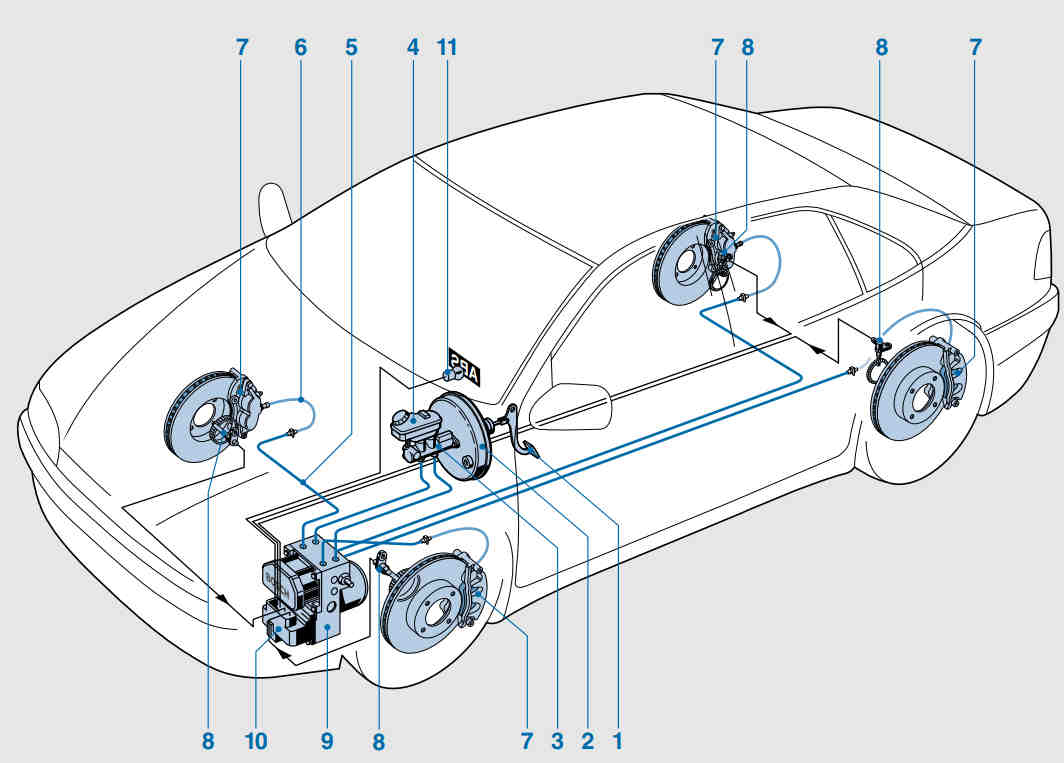
\includegraphics[width=0.8\textwidth]{figuras/sistema-de-freio-com-abs.jpg}
    \fonte{ O Autor, adaptado de \cite{Konrad2014}.}
\end{figure}


Outra parte a ser destacada desse sistema é a parte hidráulica, responsável por conduzir o fluido de freio para exercer pressão na pastilha contra o disco. O uso de sistemas eletro-hidráulicos, especialmente em veículos elétricos, tem sido objeto de estudos recentes que visam otimizar o desempenho do motor e do sistema de frenagem de forma integrada \cite{MotorParametricDesign2023}.

 \begin{figure}[htbp]
    \centering
    \caption{Princípio do Bloco Hidráulico com Válvulas Solenoides}
    \label{fig:principio-do-modulador-hidraulico-com-valvulas-solenoides}
    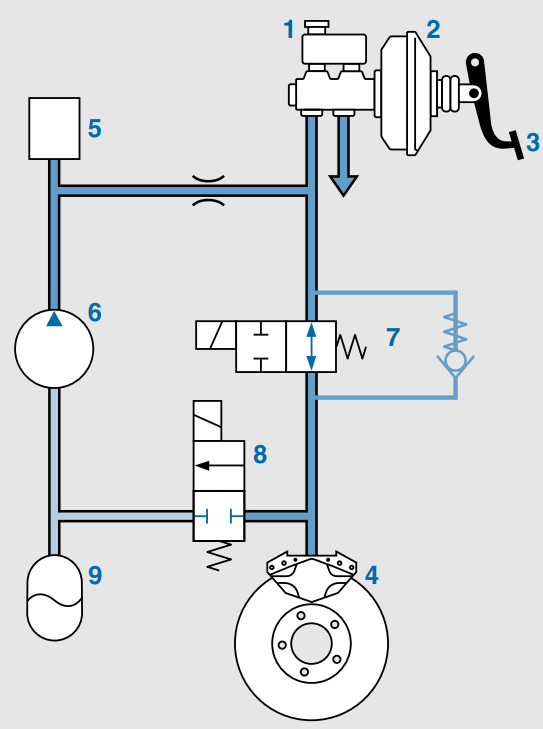
\includegraphics[width=0.8\textwidth]{figuras/principio-do-modulador-hidraulico-com-valvulas-solenoides.png}
    \fonte{ O Autor, adaptado de \cite{Konrad2014}.}
\end{figure}

 
O bloco hidráulico incorpora múltiplas válvulas solenoides que abrem ou fecham caminhos hidráulicos entre o cilindro mestre/suprimento, o retorno e os canais de roda, como mostra a Figura~\ref{fig:principio-do-modulador-hidraulico-com-valvulas-solenoides}. 

%Ele também conecta os freios à bomba de retorno (6). Válvulas solenoides com duas conexões hidráulicas e duas posições de válvula são usadas (válvulas solenoides 2/2). A válvula de entrada (7), entre o cilindro mestre e o freio, controla a aplicação de pressão, enquanto a válvula de saída (8), entre o freio e a bomba de retorno, controla a liberação de pressão. Há um par de válvulas solenoides para cada freio.

Ele também conecta os freios à bomba de retorno (6). Válvulas solenoides com duas conexões hidráulicas e duas posições de válvula são usadas (válvulas solenoides 2/2). A válvula de entrada (7), entre o cilindro mestre e o freio, controla a vazão de entrada de fluido para o circuito de freio, enquanto a válvula de saída (8), entre o freio e a bomba de retorno, controla a \textbf{vazão de saída} do fluido para o reservatório de baixa pressão. Há um par de válvulas solenoides para cada freio.


\subsection{Válvulas Solenoide}
\label{sec:metodologia-4-1}

As válvulas são indispensáveis, porque modulam a pressão do sistema.
A Figura~\ref{fig:modelo-hidraulico-conjunto-freio} apresenta o modelo hidráulico com o conjunto de freio automotivo.

 \begin{figure}[htbp]
    \centering
    \caption{Modelo Hidráulico com Conjunto de Freio Automotivo.}
    \label{fig:modelo-hidraulico-conjunto-freio}
    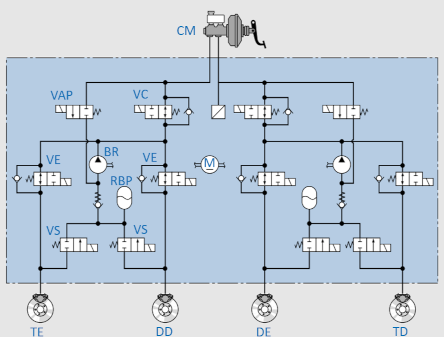
\includegraphics[width=0.8\textwidth]{figuras/modelo-hidraulico-conjunto-freio.png}
    \fonte{ O Autor, adaptado de \cite{Konrad2014}.}
\end{figure}

O processo de modulação hidráulica em unidades ABS/ESC pode ser descrito, de forma funcional, pelos três modos clássicos de atuação no canal/roda: \textit{aumento de pressão} (pressurização), \textit{retenção} (\textit{hold}) e \textit{redução de pressão} (alívio). Em termos hidráulicos, esses modos decorrem da combinação de estados das válvulas de entrada (que estabelecem ou bloqueiam a comunicação com o suprimento) e de saída (que estabelecem ou bloqueiam a comunicação com o retorno), bem como do acionamento do conjunto motor+bomba.

No \textbf{ABS clássico} (frenagem comandada pelo condutor), a pressão base é gerada no cilindro mestre e a unidade hidráulica atua modulando-a por roda, tipicamente com recirculação para recomposição de pressão. Já em \textbf{frenagem ativa} (ESC/ADAS), a unidade eletro-hidráulica pode assumir o papel de atuador principal de pressão, impondo perfis de pressão por roda a partir de uma referência gerada eletronicamente. Esse é o modo de interesse deste trabalho.

\subsection{Motor da Bomba de Pressão}
\label{sec:metodologia-4-2}
A função do conjunto motor+bomba é fornecer vazão ao suprimento e permitir a recomposição/geração de pressão hidráulica necessária para a modulação por canal. Em ABS/ESC, esse conjunto pode operar tanto para recirculação (recomposição durante modulação) quanto, em arquiteturas de frenagem ativa, como fonte primária de pressão para impor perfis de pressão por roda.

%A bomba normalmente consiste em um motor, geralmente BLDC (que significa \textit{Brushless Direct Current}, que se traduz para corrente contínua sem escovas) e um pistão ou diafragma para criar pressão. Quando o sistema ABS ou ESP detecta uma trava potencial de roda, ou perda de tração, a bomba é ativada para ajustar a pressão do freio rapidamente. Isso garante o desempenho ideal de frenagem e o controle do veículo.

A bomba utilizada em sistemas ABS ou de controle de estabilidade (ESC/ESP) tipicamente não é do tipo engrenagem, mas sim uma bomba de pistão alternativo acionada por um motor elétrico, normalmente do tipo BLDC (\textit{Brushless Direct Current}). Esse motor aciona um mecanismo excêntrico que movimenta o pistão da bomba, permitindo recircular o fluido e restabelecer a pressão no circuito.

O elemento responsável por armazenar fluido sob pressão — frequentemente um acumulador hidráulico, que pode ser do tipo pistão ou diafragma — não deve ser confundido com a bomba. Quando o sistema ABS ou ESC/ESP detecta uma potencial perda de tração, ou iminência de travamento da roda, a bomba pode ser acionada para recompor a pressão rapidamente, contribuindo para o desempenho de frenagem e a estabilidade do veículo.


\subsection{Sensor da Roda}
\label{sec:metodologia-4-3}

Os sensores de velocidade da roda são usados para medir a velocidade de rotação das rodas do veículo. Esses sinais são fundamentais para funções como ABS e ESC, nas quais a unidade de controle estima condições de escorregamento e estabilidade e decide intervenções de frenagem. No presente trabalho, entretanto, o foco da avaliação em simulação está no \textbf{regulador de pressão hidráulica} (atuador), de modo que os sensores de roda são tratados principalmente como parte da arquitetura típica do sistema e como motivação para a plataforma eletrônica proposta. Além disso, de acordo com \citeonline{Konrad2014}, sistemas de navegação também podem usar sinais de velocidade da roda para estimar distância percorrida (por exemplo, em túneis). Normalmente encontram-se sensores de velocidade da roda em dois modelos: passivos e ativos.

\subsubsection{Sensor da Roda Modelo Passivo}
\label{sec:metodologia-4-3-1}

Um sensor passivo (indutivo) consiste em um ímã permanente (1) com um pino de pólo magnético macio (3) conectado a ele, inserido em uma bobina (2) com vários enrolamentos de areia. Essa configuração gera um campo magnético constante (5). O pino do poste é instalado diretamente acima da roda do pulso (4). A Figura~\ref{fig:diagrama-de-sensor-passivo-e-sinal-gerado} apresenta o funcionamento do sensor e o sinal gerado.

 \begin{figure}[htbp]
    \centering
    \caption{Diagrama de Sensor Passivo e Sinal Gerado.}
    \label{fig:diagrama-de-sensor-passivo-e-sinal-gerado}
    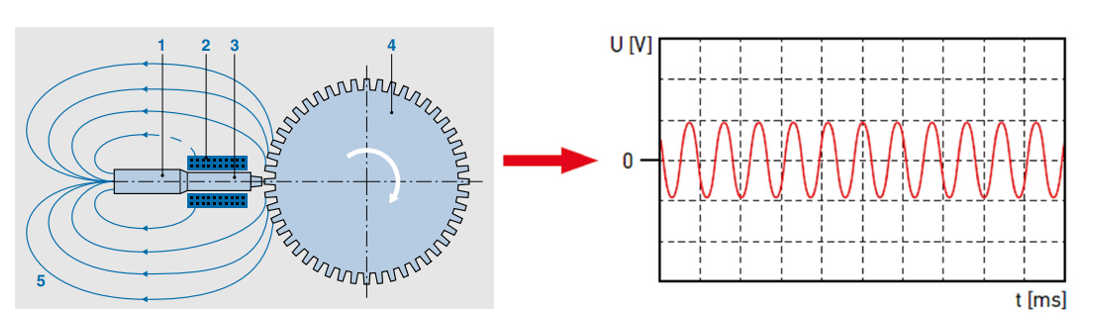
\includegraphics[width=0.8\textwidth]{figuras/diagrama-de-sensor-passivo-e-sinal-gerado.jpg}
    \fonte{ O Autor, adaptado de \cite{Konrad2014}.}
\end{figure}

\subsubsection{Sensor da Roda Modelo Ativo}
\label{sec:metodologia-4-3-2}

Os sensores ativos são usados quase que exclusivamente nos modernos sistemas de freio atuais \cite{Konrad2014}. Esses sensores geralmente consistem em um \gls{CI} circuito integrado hermético de silício de plástico que fica na ponta do sensor(1).  Neste modelo a resistência elétrica muda à medida que o campo magnético muda, e, este comportamento é devido a um anel multipolar(2) usado como uma roda de pulso para sensor. Esses sensores reagem às menores alterações no campo magnético e, portanto, permitem maiores lacunas de ar em comparação com sensores passivos de velocidade da roda, como mostra a Figura~\ref{fig:diagrama-de-sensor-ativo-e-sinal-gerado}.

\begin{figure}[htbp]
    \centering
    \caption{Diagrama de Sensor Ativo e Sinal Gerado.}
    \label{fig:diagrama-de-sensor-ativo-e-sinal-gerado}
    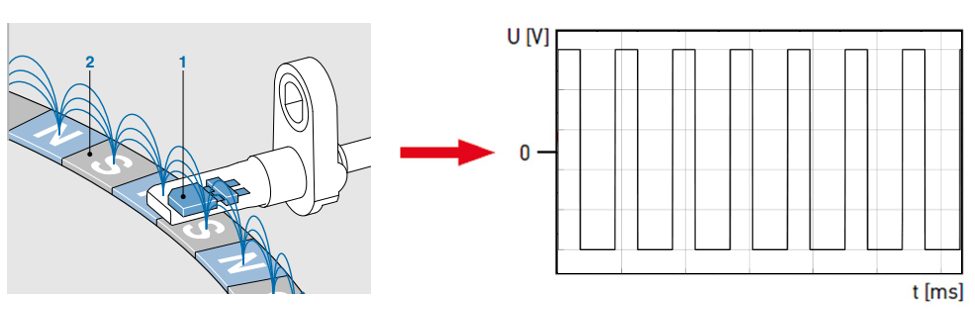
\includegraphics[width=0.8\textwidth]{figuras/diagrama-de-sensor-ativo-e-sinal-gerado.png}
    \fonte{ O Autor, adaptado de \cite{Konrad2014}.}
\end{figure}


\section{Sensor de Pressão de Óleo}
\label{sec:metodologia-5}

O sistema de freio do veículo é complexo e pode concentrar múltiplas válvulas no modulador hidráulico (por exemplo, 12 válvulas em arquiteturas ABS/ESC), sendo que parte delas atua sob alta pressão e diferenciais de pressão elevados (superiores a aproximadamente 0{,}1~MPa, isto é, 1~bar) \cite{Konrad2014}.
Também vale ressaltar que, em estratégias de controle de estabilidade (ESC/ESP), a modulação de pressão de freio por roda é utilizada para contribuir com a estabilidade do veículo por meio de intervenções seletivas de frenagem.

Em veículos com ESC/ESP, é comum a presença de um sensor de pressão para monitorar a pressão hidráulica (por exemplo, associada ao cilindro mestre ou ao circuito), permitindo estimar a ação do condutor e apoiar funções de controle e diagnóstico.

Em aplicações ADAS de controle longitudinal (por exemplo, ACC/AEB), a referência de desaceleração/torque pode ser convertida em uma referência de pressão; quando disponível, a medição de pressão contribui para o fechamento de malha e para a avaliação do desempenho do atuador hidráulico.

\begin{figure}[htbp]
    \centering
    \caption{Sensor de Pressão no Bloco do Sistema de Freio.}
    \label{fig:bloco-do-sistema-de-freio}
    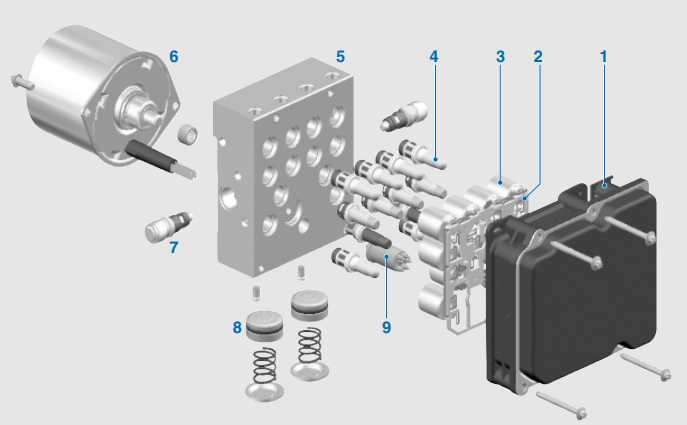
\includegraphics[width=0.8\textwidth]{figuras/bloco-do-sistema-de-freio.jpg}
    \fonte{ O Autor, adaptado de \cite{Konrad2014}.}
\end{figure}

\section{Desenvolvimento da Placa de Controle}
\label{sec:metodologia-6}

O desenvolvimento da placa, tem origem na necessidade de haver um controle das partes relacionadas ao freio, ou seja, o módulo de freio recebe sinais diretamente de sensores ou componentes conectados fisicamente a ele. Isso é mais comum em sistemas críticos que exigem baixa latência ou alta confiabilidade, como sensores de velocidade das rodas, sensores de pressão do freio, e sensores de pedal de freio. 

\begin{figure}[htbp]
    \centering
    \caption{Diagrama em Bloco da Placa Proposta.}
    \label{fig:diagrama-em-bloco-da-placa-proposta}
    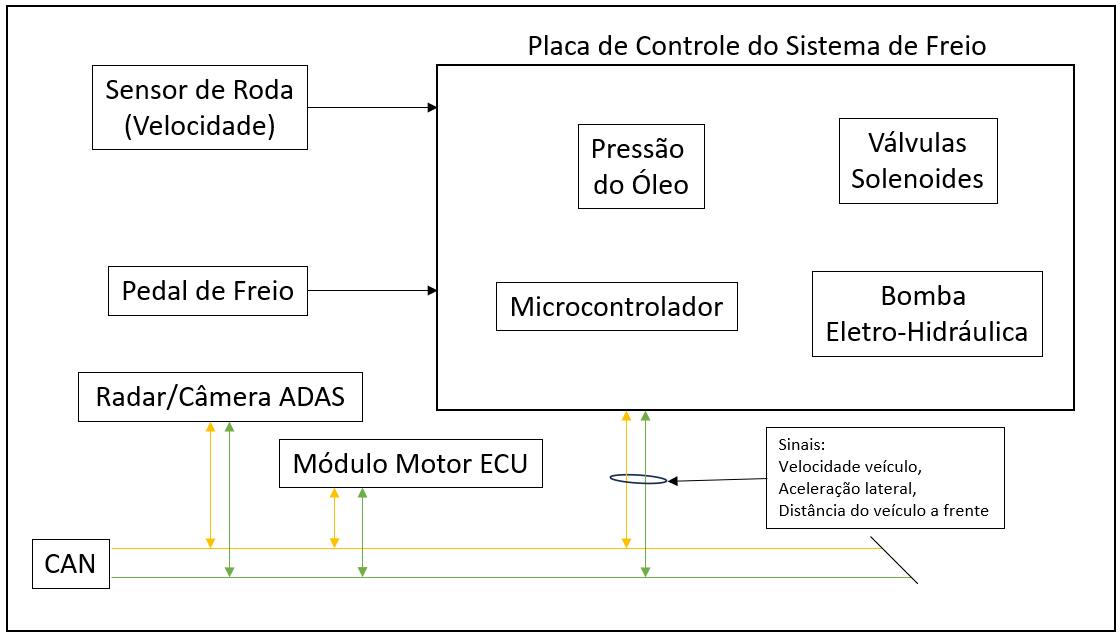
\includegraphics[width=0.8\textwidth]{figuras/diagrama-em-bloco-da-placa-proposta.png}
    \fonte{ O Autor.}
\end{figure}

Também os componentes são controlados para garantir a segurança, estabilidade e eficiência do veículo, como "atuadores de pressão de freio", que controlam a pressão de freio em cada roda; em outras palavras, uma bomba eletro-hidráulica, capaz de gerar pressão de freio independentemente; e ainda, válvulas moduladoras	que regulam a pressão de freio em cada roda e por fim,  um motor de freio de estacionamento, para controlar o freio de estacionamento eletronicamente. A Figura~\ref{fig:diagrama-em-bloco-da-placa-proposta}, apresenta o diagrama em bloco da placa proposta.

\subsection{Circuitos Propostos}
\label{sec:metodologia-6-1}

Os circuitos responsáveis pelo condicionamento de sinais, acionamento de válvulas, controle da bomba e leitura de sensores foram projetados de acordo com os requisitos de baixa latência, compatibilidade elétrica e robustez frente a ruído. 

Cada circuito cumpre uma função específica dentro da plataforma experimental: 
\begin{enumerate}
    \item  condicionamento do sinal do sensor de velocidade,
    \item  acionamento das válvulas solenoides,
    \item  controle do motor da bomba eletro-hidráulica e
    \item  leitura do sensor de pressão.
\end{enumerate}


\begin{comment}
% Comentei essa area, porque nao tinha o appendice referenciado. 
A descrição completa desses circuitos, incluindo seus esquemáticos, diagramas elétricos e simulações, encontra-se no Apêndice~\ref{ap:circuitos-propostos}.


    
\subsection{Circuitos Propostos}
\label{sec:metodologia-6-1}

Para condicionar o sinal proveniente do sensor de velocidade, foi definido um circuito comparador Figura~\ref{fig:circuito-sensor-de-roda-proposto}, uma vez que o sinal pode apresentar ruído e pode ser de uma magnitude baixa, o circuito comparador é ideal neste cenário, por utilizar um amplificador operacional, que possui alta impedância na sua entrada.

Para o condicionamento do sinal proveniente do sensor de velocidade, foi adotado um circuito comparador baseado em amplificador operacional. Esse circuito é responsável por elevar a robustez do sinal e garantir níveis de tensão compatíveis com o microcontrolador utilizado. A descrição completa do circuito, incluindo seu diagrama e análise de funcionamento, encontra-se no Apêndice~\ref{ap:circuito-sensor-roda}.

\begin{figure}[htbp]
    \centering
    \caption{Circuito Sensor de Roda Proposto.}
    \label{fig:circuito-sensor-de-roda-proposto}
    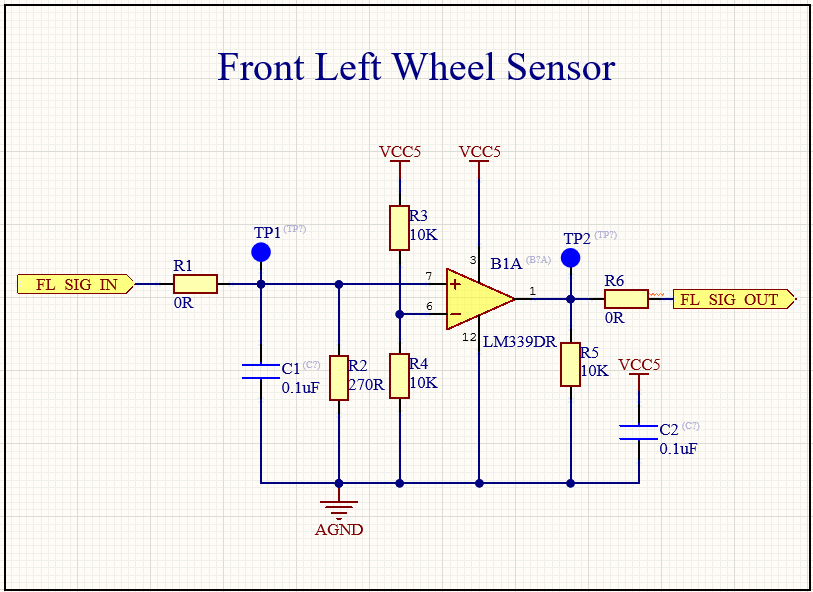
\includegraphics[width=0.8\textwidth]{figuras/circuito-sensor-de-roda-proposto.png}
    \fonte{ O Autor.}
\end{figure}

Foi inserido um comparador que limita a tensão em 2.5V, ou seja, quando o sinal do sensor estiver no ciclo positivo, a saída do amplificar será nível alto lógico, que no caso do microcontrolador escolhido é de 3V3, e quando o sinal do sensor estiver no nível baixo, ou seja, abaixo de 2.5V o sinal será 0V para o microcontrolador, como mostra a simulação do circuito no LTSpice da Figura~\ref{fig:simulacao-circuito-sensor-de-roda-proposto}.

\begin{figure}[htbp]
    \centering
    \caption{Simulação do Circuito Sensor de Roda Proposto.}
    \label{fig:simulacao-circuito-sensor-de-roda-proposto}
    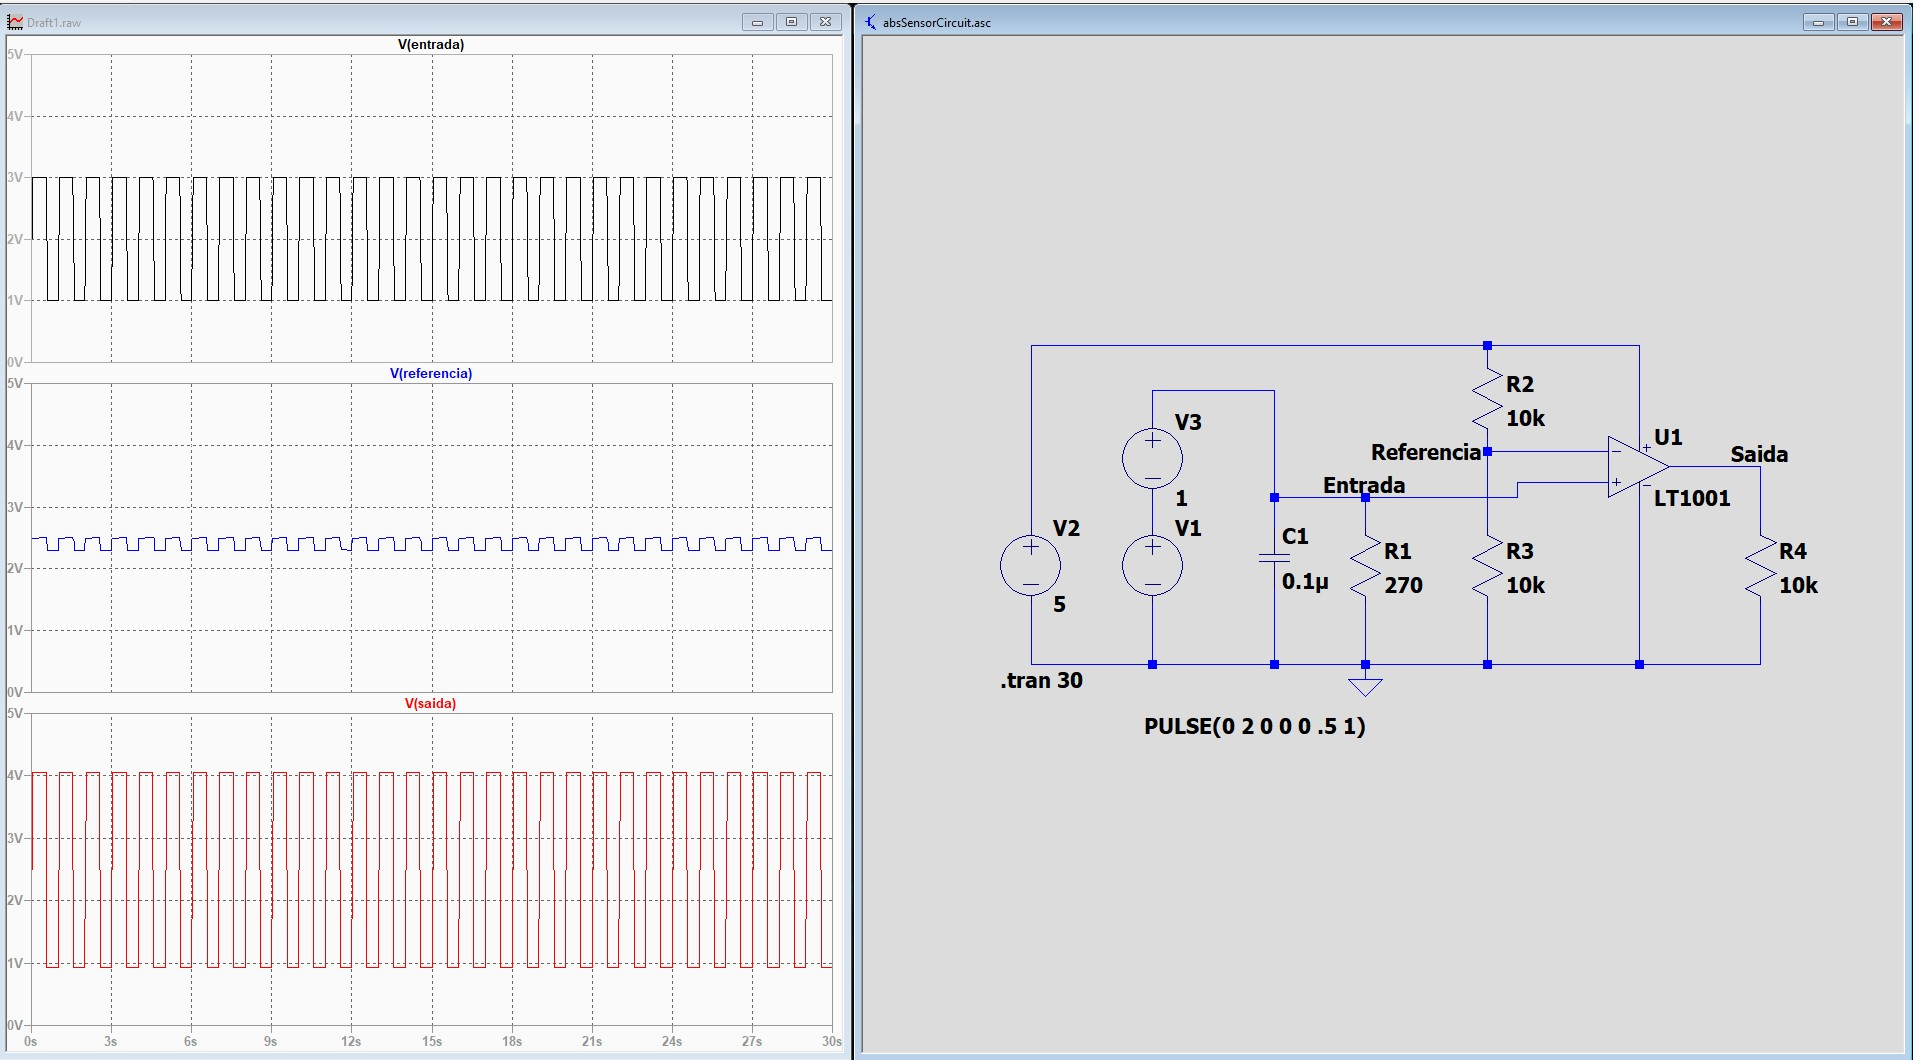
\includegraphics[width=0.8\textwidth]{figuras/simulacao-circuito-sensor-de-roda-proposto.jpg}
    \fonte{ O Autor.}
\end{figure}

\subsection{Circuito da Válvula}
\label{sec:metodologia-6-2}

O circuito da placa, tem como base o kit de Freio da NXP, o KITVALVECNTLEVM \cite{KITVALVECNTLEVM}. Esse kit possui 2 Circuitos Integrados (CI), o MC34SB0800 tem a capacidade de controlar 8 válvulas e um motor, e o MC34SB0410 controla 4 válvulas e um motor. 

O circuito foi totalmente baseado no kit \citeonline{KITVALVECNTLEVM} Figura~\ref{fig:circuito-controle-valvula-solenoide}.
 
\begin{figure}[htbp]
    \centering
    \caption{Circuito de Controle das Válvulas Solenoides.}
    \label{fig:circuito-controle-valvula-solenoide}
    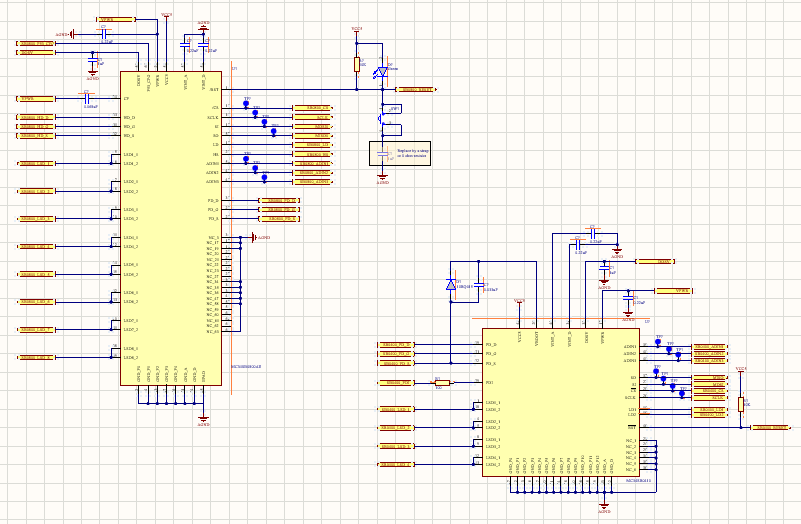
\includegraphics[width=0.8\textwidth]{figuras/circuito-controle-valvula-solenoide.png}
    \fonte{ O Autor adaptado de \cite{MC34SB0800}. }
\end{figure}

\subsection{Circuito da Bomba}
\label{sec:metodologia-6-3}

 O circuito proposto, foi baseado no kit \cite{KITVALVECNTLEVM}, a operação do motor da bomba, se faz ao selecionar o drive de controle, tendo em vista que o MC34SB0800 suporta controle de alta frequência de até 500 Hz \gls{PWM} \cite{MC34SB0800}, enquanto isso, o MC34SB0410 pode lidar com frequências PWM de até 16 kHz, fornecendo operação mais silenciosa e controle mais fino \cite{MC34SB0410}.

Ambos os drives contam com proteções de corrente, para manter a integridade do circuito da Figura~\ref{fig:circuito-controle-valvula-motor}.

\begin{figure}[htbp]
    \centering
    \caption{Circuito de Controle da Bomba de pressão.}
    \label{fig:circuito-controle-valvula-motor}
    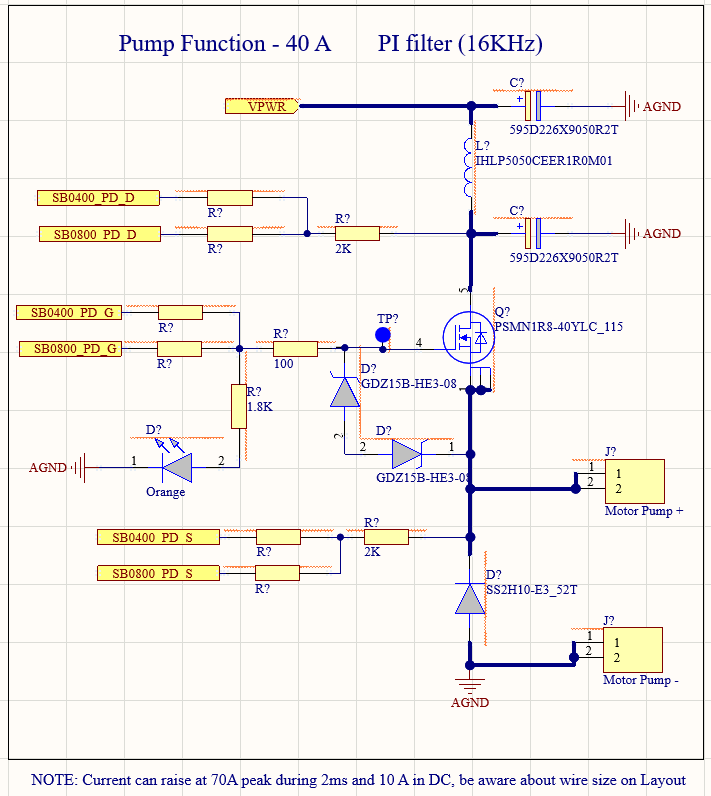
\includegraphics[width=0.8\textwidth]{figuras/circuito-controle-valvula-motor.png}
    \fonte{ O Autor adaptado de \cite{MC34SB0800}. }
\end{figure}

\subsection{Circuito Sensor de Pressão}
\label{sec:metodologia-6-4}

No mercado atual, entre os modelos de sensores encontrados, foram eleitos os sensores piezoresistivos ou tipo \textit{strain gauge}, devido a criticidade desse componente aplicado no sistema de freio, para mitigar uma possível falha de leitura. Também foi decisiva a escolha de circuito de amplificador de instrumentação, por ser menos suscetivo a ruído em seu condicionamento, a Figura~\ref{fig:circuito-sensor-de-pressao-proposto} mostra o circuito para fazer a leitura deste sensor. 

\begin{figure}[htbp]
    \centering
    \caption{Circuito de Leitura do Sensor de Pressão.}
    \label{fig:circuito-sensor-de-pressao-proposto}
    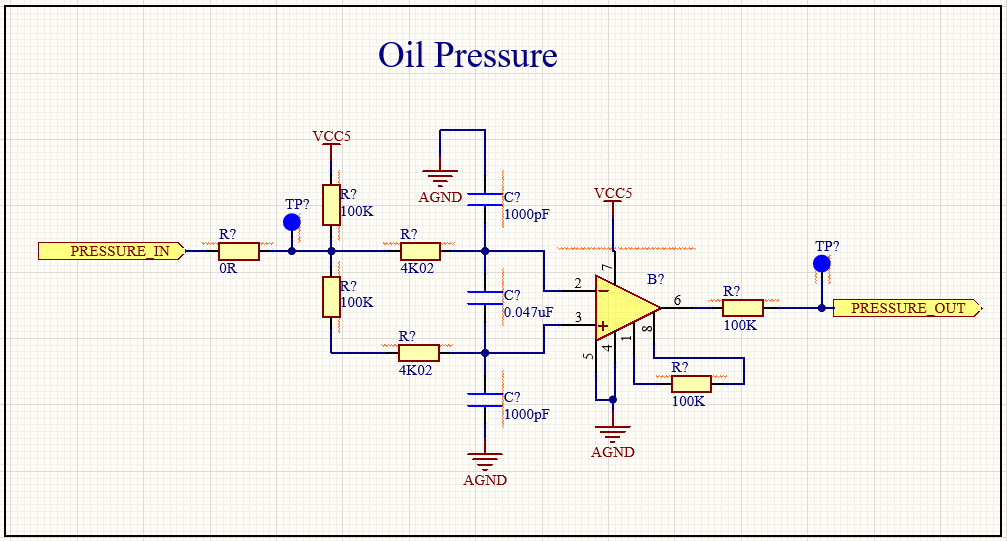
\includegraphics[width=0.8\textwidth]{figuras/circuito-sensor-de-pressao-proposto.png}
    \fonte{ O Autor. }
\end{figure}

\end{comment}

\subsection{Microcontrolador}
\label{sec:metodologia-6-5}

Este projeto tem como base o microcontrolador AURIX TC375 \cite{tc37xDatasheet}, desenvolvido pela empresa \textit{Infineon Technologies}. Corresponde a um microcontrolador multinúcleo para aplicações automotivas devido ao seu alto desempenho; sendo essa uma das principais características, que contribuíram na definição dessa família, além de seu sistema crítico de segurança, ainda mais considerando o campo de frenagem. 
De modo que, abaixo estão elencadas as principais características do microcontrolador AURIX TC375 e, como se encaixa em um sistema de freio em termos de segurança, tecnologia e robustez:

\begin{itemize}
    \item \textbf{Arquitetura multinúcleo:} baseada em CPUs TriCore de 32 bits que operam em sincronia para redundância e tolerância a falhas.
     \item \textbf{Recursos de segurança: } projetado para atender ao mais alto nível de integridade de segurança automotiva (ASIL-D) conforme ISO 26262.
      \item \textbf{Mecanismos de segurança de hardware:} inclui códigos de correção de erros (ECC), unidades de proteção de memória (MPU) e temporizadores \textit{watchdog} para detectar e mitigar falhas.
       \item \textbf{Desempenho:} altas velocidades de \textit{clock} (até 300 MHz) e aceleradores de cálculos complexos, também possui \gls{DSP} (\textit{Digital Signal Processing}) integrados para processamento de sinal em tempo real.
\end{itemize}

Como descrito, este microcontrolador é muito relevante, mas isso não significa que poderia ser empregado unicamente ele na placa, uma vez que, adicionalmente ao microcontrolador AURIX TC375 (INFINEON, 2021), também foi implementada uma conexão na placa visando conectar o Kit de desenvolvimento do TC375\_LITE \cite{tc37xEvaluationBoard}. 

Além disso, uma característica fundamental da placa proposta, é que ela seja flexível quanto ao microcontrolador usado, por esse motivo, foi adicionada uma conexão compatível com Arduino, permitindo desenvolver essa placa com qualquer kit de desenvolvimento desde que com a mesma estrutura.

Durante o desenvolvimento do projeto, o TC375 é responsável pela aquisição dos sinais fornecidos pelo sensor de roda e pelo sensor de pressão. Adicionalmente, uma vez que o kit de desenvolvimento incorpora um \textit{transceiver CAN} baseado no \gls{TLE9251VSJ}, o sistema é capaz de receber informações por meio da rede \gls{CAN}.

A partir de todos os detalhes apresentados, é possível notar que o controle é capaz de definir o exato momento para fazer o acionamento das válvulas e do motor de pressão. 


\subsection{Protocolo de Comunicação CAN}
\label{sec:metodologia-6-6}

 O protocolo \textit{Controller Area Network} (CAN) tem sido amplamente adotado na indústria automotiva e de automação desde sua introdução em 1991 \cite{wiley2022}. Ele proporciona uma comunicação eficiente e confiável entre unidades de controle eletrônico (ECUs), sensores e atuadores, garantindo integridade dos dados e tolerância a falhas. Operando com uma arquitetura multi-mestre, o CAN permite a transmissão de mensagens com base em prioridade, utilizando um sistema de arbitragem que assegura que a mensagem mais importante seja enviada sem colisões. 
 
 A comunicação ocorre por meio de um barramento diferencial de dois fios (CAN\_H e CAN\_L), reduzindo interferências eletromagnéticas e assegurando a robustez da transmissão.
 
 Além disso, o protocolo inclui diversos mecanismos de detecção e correção de erros, como o Cíclico de Redundância (CRC) e a técnica de bit \textit{stuffing}, que garantem a confiabilidade dos dados.
 
 Outrossim, avanços como o \textit{Time-Triggered} CAN (TTCAN) e o CAN com Taxa de Dados Flexível (CAN-FD) ampliaram a aplicabilidade do protocolo, possibilitando transmissões mais rápidas e eficientes, atendendo às exigências dos modernos sistemas automotivos conectados e autônomos.

\section{Demonstração do Funcionamento}
\label{sec:metodologia-7}
Foram realizados testes em simulação para demonstrar o comportamento do sistema e verificar a viabilidade da estratégia de controle no ambiente MATLAB/Simulink. Em paralelo, foi desenvolvido um protótipo de placa eletrônica com foco em viabilizar a futura migração do controlador para execução embarcada e ensaios em bancada.

No escopo deste trabalho, não é apresentada a validação prática do controle em um conjunto físico de freio; essa etapa permanece como continuação natural, conforme discutido no Capítulo~\ref{chap:resultados}.

\section{Descrição dos Instrumentos e Procedimentos}
\label{sec:metodologia-8}
Os instrumentos e ferramentas utilizados incluem o ambiente MATLAB/Simulink para modelagem e simulação, rotinas MATLAB para parametrização e pós-processamento, e a documentação da plataforma eletrônica baseada no microcontrolador AURIX TC375. Os procedimentos incluem: (i) modelagem matemática da planta hidráulica, (ii) implementação do controle digital e da lógica de atuação no Simulink, (iii) registro dos sinais de interesse e (iv) análise dos resultados para diferentes cenários simulados (por exemplo, perfis de referência em patamares e ensaios em malha aberta).

\section{Critérios de Validação}
\label{sec:metodologia-9}
A validação do sistema é conduzida por meio da análise de métricas de desempenho (por exemplo, tempo de subida e de acomodação, sobressinal, erro RMS e erro estacionário), além de inspeção das saturações e do esforço de atuação dos comandos. Essas métricas são calculadas a partir dos sinais registrados no Simulink, conforme detalhado no Capítulo~\ref{chap:resultados}.

Quando aplicável, discute-se a coerência de ordens de grandeza (pressão e vazão) em relação a faixas reportadas na literatura. A conformidade com normas e procedimentos de homologação e a comparação quantitativa com \emph{benchmarks} experimentais ficam fora do escopo deste trabalho.

\section{Simulações: Parâmetros, Modelos e Ferramentas}
\label{sec:metodologia-10}
As simulações foram conduzidas no ambiente MATLAB/Simulink, utilizando modelos matemáticos formulados a partir de equações diferenciais ordinárias e representados no formalismo de espaço de estados. Parâmetros como massa do veículo, pressão hidráulica, frequência de modulação por largura de pulso (PWM) e características dos atuadores foram ajustados visando avaliar o desempenho do sistema sob diferentes condições operacionais.

\section{Desenho Experimental, Amostragem e Análise Estatística}
\label{sec:metodologia-11}
Os ensaios apresentados neste trabalho são baseados em cenários determinísticos de simulação, definidos por perfis de referência e condições de operação do modelo. Dessa forma, a análise é conduzida principalmente por curvas e métricas de desempenho extraídas dos \emph{logs} do Simulink.

Uma avaliação estatística formal (múltiplas execuções com variação sistemática de parâmetros e ruídos, com cálculo de médias e dispersões) é um desdobramento possível para trabalhos futuros, sobretudo em conjunto com validação experimental.

\section{Limitações e Possíveis Vieses}
\label{sec:metodologia-12}
Entre as limitações do estudo, destacam-se restrições do ambiente de simulação, simplificações adotadas nos modelos matemáticos e a ausência de validação do controle em hardware e no conjunto físico de freio. Além disso, ruídos, quantização e atrasos de sensores/atuadores não são explorados de forma exaustiva em todos os cenários.

Como continuidade, recomenda-se a realização de estudos complementares em bancada e/ou em plataformas \textit{hardware-in-the-loop} para validação experimental, conforme discutido na literatura \citeonline{Lv2014}, além de análises de sensibilidade a variações paramétricas e ruídos para consolidar robustez.
% !TeX root = ../documento.tex
\chapter{Metodologia específica: controle do sistema hidráulico não linear}
\label{cap:controle}

Este capítulo apresenta a metodologia adotada para o projeto e a avaliação, em simulação, de uma estratégia de controle digital de pressão de freio que utiliza o módulo hidráulico de uma unidade ABS/ESC como atuador de pressão do freio de serviço. O estudo é desenvolvido em ambiente simulado, com possibilidade de extensão para ensaios em bancada, considerando um canal/roda (modelo concentrado em duas pressões) e implementação digital em tempo discreto, com faixas de pressão compatíveis com a aplicação e período de amostragem compatível com ECUs automotivas.

O foco é o seguimento de uma referência de pressão por roda, que pode ser obtida a partir de um controlador longitudinal de nível superior (por exemplo, um ACC), e a avaliação do compromisso entre desempenho dinâmico e esforço de atuação imposto pelas limitações físicas do módulo hidráulico.

O problema de pesquisa é formulado da seguinte maneira: como projetar e implementar um controlador digital em espaço de estados que permita ao módulo hidráulico ABS/ESC rastrear perfis de pressão $P_{\mathrm{ref}}(t)$ por roda, garantindo desempenho dinâmico adequado e esforço de atuação compatível com as limitações físicas do sistema?

A hipótese considerada é que um controlador LQ em tempo discreto (LQI) com observador de Luenberger, sintetizado a partir da linearização local de um modelo não linear em duas pressões, é capaz de rastrear referências de pressão por roda com erro estacionário nulo e dinâmica satisfatória, desde que: (i) o ponto de operação satisfaça $\Delta P>0$ nas válvulas, (ii) as saturações sejam parametrizadas de forma fisicamente consistente e (iii) o período de amostragem seja compatível com a banda do atuador.

O objetivo geral é demonstrar, em simulação, que o módulo hidráulico ABS/ESC pode atuar como atuador principal de pressão do freio de serviço, acompanhando perfis $P_{\mathrm{ref}}(t)$ consistentes com requisitos de desaceleração.

Os objetivos específicos são:
\begin{enumerate}
    \item Modelar o subsistema hidráulico por um modelo não linear em duas pressões ($P_{sup},P_w$) e realizar uma validação qualitativa em malha aberta.
    \item Linearizar o modelo em torno de um ponto de operação $(x_0,u_0)$ fisicamente consistente, obtendo as matrizes $(A,B,C,D)$.
    \item Discretizar o sistema e projetar um controlador LQI discreto, com observador de Luenberger, para regular a velocidade da bomba ($\omega_p$), em conjunto com uma lógica discreta (on/off com histerese) para as válvulas de entrada e saída.
    \item Avaliar o seguimento de $P_{\mathrm{ref}}(t)$ e o esforço de controle sob saturações físicas de pressão e dos atuadores.
\end{enumerate}

O capítulo está organizado da seguinte forma: inicialmente define-se como a referência de pressão $P_{\mathrm{ref}}(t)$ é especificada nos ensaios (incluindo um mapeamento simples a partir de desaceleração, quando aplicável) (Seção~\ref{sec:mapeamento-aref-pressao}) e descreve-se o modelo hidráulico não linear 2P (Seção~\ref{sec:controle-4-1}); em seguida, apresenta-se a linearização e a formulação em espaço de estados (Seções~\ref{sec:controle-linearizacao-2p} e \ref{sec:controle-formulacao-espaço-estados}); por fim, descrevem-se a síntese do controlador/observador, a discretização e a implementação em Simulink (Seções~\ref{sec:controle-lqr-luenberger} a \ref{sec:implementacao-simulink}). Os procedimentos de simulação e as métricas adotadas são resumidos na Seção~\ref{sec:procedimentos-simulacao-controle}, e os resultados são apresentados e discutidos no Capítulo~\ref{chap:resultados}.


%====================================================================
%====================================================================
%====================================================================
%====================================================================
\section{Da desaceleração à referência de pressão por roda}
\label{sec:mapeamento-aref-pressao}
Neste capítulo, a referência de pressão $P_{\mathrm{ref}}(t)$ é tratada como uma entrada do ensaio (isto é, um sinal especificado externamente ao regulador de pressão), pois o objetivo aqui é isolar e avaliar a dinâmica do módulo hidráulico sob controle. Na integração com uma função ADAS de nível superior (por exemplo, um ACC), é natural que o nível longitudinal forneça um requisito em termos de desaceleração desejada $a_{\mathrm{ego}}(t)$; nesse caso, é necessário algum procedimento que converta desaceleração em referência de pressão por roda.

Como este trabalho não tem por objetivo identificar ou validar um modelo completo de veículo/pneu/freio, adota-se um mapeamento propositalmente simples, suficiente para gerar sinais de referência coerentes (em ordem de grandeza) para os ensaios em Simulink. A ideia é aplicar pressão apenas quando houver solicitação de frenagem e usar um ganho agregado que concentre, em um único parâmetro, os efeitos de repartição por roda, transferência de carga e eficiência do conjunto de freio.

Assume-se, de forma agregada, que a demanda de força longitudinal de frenagem pode ser aproximada por uma relação proporcional com a pressão no canal/roda (pressão manométrica relativa ao retorno),
\begin{equation}
    F_{x,\mathrm{eq}}(t) = A_c\,P_{\mathrm{ref}}(t),
    \label{eq:fxeq_ac_pref}
\end{equation}
em que $F_{x,\mathrm{eq}}(t)$ é uma força equivalente de frenagem e $A_c$ (unidade de área) agrega os efeitos de repartição por roda, conversão pressão--força no atuador, raio efetivo e eficiência do conjunto de freio. Com $F_{x,\mathrm{eq}}(t)\approx m\,\max\big(-a_{\mathrm{ego}}(t),0\big)$, obtém-se o mapeamento simples:
\begin{equation}
    P_{\mathrm{ref}}(t) = \frac{m}{A_c}\,\max\big( -a_{\mathrm{ego}}(t),\,0\big).
    \label{eq:mapeamento_aref_pressao}
\end{equation}
Na prática, os valores de $m$ e $A_c$ são escolhidos para produzir níveis de pressão compatíveis com a faixa de operação considerada no modelo hidráulico. A rotina utilizada para gerar $P_{\mathrm{ref}}$ a partir de $a_{\mathrm{ego}}(t)$ é apresentada no Apêndice~\ref{ap:codigos-matlab}, na Listagem~\ref{lst:accel-to-pressure}.

%====================================================================
%====================================================================
%====================================================================
%====================================================================
\section{Modelo hidráulico não linear de duas pressões}
\label{sec:controle-4-1}
A planta controlada é o módulo hidráulico da unidade ABS/ESC, empregado como atuador de pressão do freio de serviço. A literatura indica a utilidade de modelos concentrados para descrever a relação entre comandos de válvulas, pressão no cilindro da roda e força de frenagem, tanto para projeto de controladores quanto para validação \emph{hardware-in-the-loop} \cite{HouhuaJing2022,PressureCoordinatedControl2023,ZengYangHuang2023,MotorParametricDesign2023}.

Neste trabalho, adota-se um modelo em duas pressões, $P_{sup}$ (suprimento/manifold) e $P_w$ (canal/roda), em linha com \citeonline{HouhuaJing2022,ZengYangHuang2023,Lv2014}.

Para fins de projeto, definem-se os vetores de estado e comando como:
\begin{equation}
    x(t) =
    \begin{bmatrix}
        P_{sup}(t) \\[2pt]
        P_{w}(t)
    \end{bmatrix},
    \qquad
    u(t) =
    \begin{bmatrix}
        \omega_p(t) \\[2pt]
        u_{in}(t)   \\[2pt]
        u_{out}(t)
    \end{bmatrix}.
    \label{eq:vect-estados-hidraulico}
\end{equation}


%====================================================================
%====================================================================
%====================================================================
%====================================================================
\subsection{Estratégias de acionamento das válvulas}
\label{sec:controle-4-1-1}

O módulo hidráulico é composto por uma bomba de deslocamento variável, válvulas de entrada (pressurização) e de saída (alívio) para cada canal/roda, e um suprimento de fluido. As válvulas podem ser do tipo on/off (solenóides) ou proporcionais (HSV/USV), o que abre diferentes possibilidades de estratégia de acionamento.

Na literatura, destacam-se duas abordagens usuais:
\begin{itemize}
    \item \textbf{Modulação quase linear de queda de pressão}: válvulas on/off operam em torno de um ponto de equilíbrio no qual a queda de pressão varia aproximadamente de forma linear com a corrente/condutância, permitindo o uso de relações vazão–comando simplificadas para projeto \cite{ChenLv2017}.
    \item \textbf{PWM em válvulas HSV/USV}: o ciclo de trabalho governa a taxa de pressurização/alívio, solução compatível com arquiteturas embarcadas e eficaz para rastreamento dinâmico de pressão \cite{HouhuaJing2022}.
\end{itemize}

Neste trabalho, o modelo matemático adota válvulas on/off e $u_{in}$ e $u_{out}$ são tratados como comandos discretos (aberto/fechado). Para evitar comutações excessivas na presença de ruído e discretização, emprega-se uma histerese sobre o erro de seguimento $e(t)=P_{w,\text{ref}}(t)-P_w(t)$ na geração desses sinais. Em uma implementação embarcada, é possível ainda interpretar $u_{in}$ e $u_{out}$ como sinais de modulação PWM (ciclo de trabalho) e adotar um modelo médio; no presente estudo, prioriza-se a lógica on/off para representar o comportamento típico de válvulas solenóides.

%====================================================================
%====================================================================
%====================================================================
%====================================================================
\subsection{Dinâmica e leis de vazão}
\label{sec:controle-modelo-hidraulico-2p}

Adota-se uma representação \emph{lumped-parameter} com duas regiões compressíveis: (i) suprimento, $P_{sup}$, volume $V_{sup}$ e retorno $P_{ret}$; (ii) canal de roda, $P_w$, volume $V_w$.

A partir da equação de continuidade para fluido compressível, obtém-se:

\begin{equation}
    \dot{P}_{sup} = \frac{\beta}{V_{sup}}\Big(Q_{pump} - Q_{in} - Q_{\text{leak},sup}\Big),
    \quad
    \dot{P}_{w} = \frac{\beta}{V_{w}}\Big(Q_{in} - Q_{out} - Q_{\text{leak},w}\Big),
    \label{eq:din_press}
\end{equation}

em que $\beta$ é o módulo volumétrico efetivo e as vazões são modeladas a seguir.

A vazão da bomba hidráulica é descrita por
\begin{equation}
    Q_{pump} = K_b\,\omega_p - K_{lb}\big(P_{sup}-P_{ret}\big),
    \label{eq:qpump_2p}
\end{equation}
em que $K_b$ agrega deslocamento e eficiência volumétrica, e $K_{lb}$ representa o vazamento interno para o retorno \cite{MotorParametricDesign2023,WangBingbing2015}.

As válvulas de entrada e de saída são modeladas por uma lei de orifício, derivada da equação de Bernoulli (forma de Torricelli) e corrigida por um coeficiente de descarga $C_d$:

\begin{equation}
    Q = C_d\,A_{ef}\,\sqrt{\frac{2\,\Delta P}{\rho}},
    \label{eq:lei-orificio}
\end{equation}

\begin{equation}
    Q_{in} = C_{d,in}\,A_{in}(u_{in})\sqrt{\frac{2\,\big(P_{sup}-P_w\big)_{+}}{\rho}},
    \qquad
    Q_{out} = C_{d,out}\,A_{out}(u_{out})\sqrt{\frac{2\,\big(P_{w}-P_{ret}\big)_{+}}{\rho}},
    \label{eq:qin_qout}
\end{equation}
em que $(\cdot)_{+}=\max(\cdot,0)$.

Adota-se $A_{in}(u_{in}) = A_{in,\max}\,u_{in}$, $A_{out}(u_{out}) = A_{out,\max}\,u_{out}$ e $u_{in},u_{out}\in[0,1]$ \cite{ProportionalPressureABS2023,Lv2014,ChenLv2017}.

Os vazamentos internos no suprimento e no canal de roda são representados por termos proporcionais à diferença de pressão em relação ao retorno:
\begin{equation}
    Q_{\text{leak},sup} = K_{ls},\big(P_{sup}-P_{ret}\big),
    \qquad
    Q_{\text{leak},w} = K_{lw},\big(P_{w}-P_{ret}\big).
    \label{eq:leaks}
\end{equation}














%====================================================================
%====================================================================
%====================================================================
%====================================================================
\subsection{Simulação em malha aberta e validação do modelo hidráulico}
\label{sec:controle-validacao-2p}
Esta subseção descreve o ensaio em malha aberta utilizado para verificar, de forma qualitativa, a causalidade do modelo e a coerência física dos transientes de pressurização, retenção e alívio, antes da inserção do controlador.

O ensaio em malha aberta é organizado por meio de um \textit{script} MATLAB associado ao modelo em Simulink. Esse \textit{script} define o horizonte de simulação e o período de amostragem, configura os parâmetros do modelo hidráulico (volumes equivalentes, coeficientes de vazão e saturações) e gera os sinais de comando da bomba e das válvulas para as três fases do ensaio (pressurização, retenção e alívio), de modo a reproduzir cenários típicos descritos na literatura \cite{ZengYangHuang2023,Lv2014,HouhuaJing2022}. Ao final de cada simulação, são registrados os perfis de pressão no suprimento e no canal de roda, bem como as vazões e os comandos de válvula, que são utilizados para visualização gráfica e cálculo de indicadores. A arquitetura geral da simulação, incluindo o modelo hidráulico, os sinais de comando $(\omega_p,u_{in},u_{out})$ e os blocos de registro de dados, é ilustrada nas Figuras~\ref{fig:bloco_matlab_function_2p} e \ref{fig:simulink_ensaio_2p}. O código completo (bloco hidráulico 2P e \textit{script} do ensaio) encontra-se no Apêndice~\ref{ap:scripts-matlab} (Códigos~\ref{cod:bloco_hidraulico_2p} e \ref{cod:ensaio_integrado_malha_aberta}).

Para o \emph{caso realista} (parâmetros ajustados conforme a Tabela~\ref{tab:parametros_hidraulico_realista_reescrita}), utiliza-se o \textit{script} do ensaio integrado em malha aberta na configuração realista, também fornecido no Apêndice~\ref{ap:scripts-matlab} (Código~\ref{cod:ensaio_integrado_malha_aberta_real}).

\begin{figure}[htbp]
    \centering
    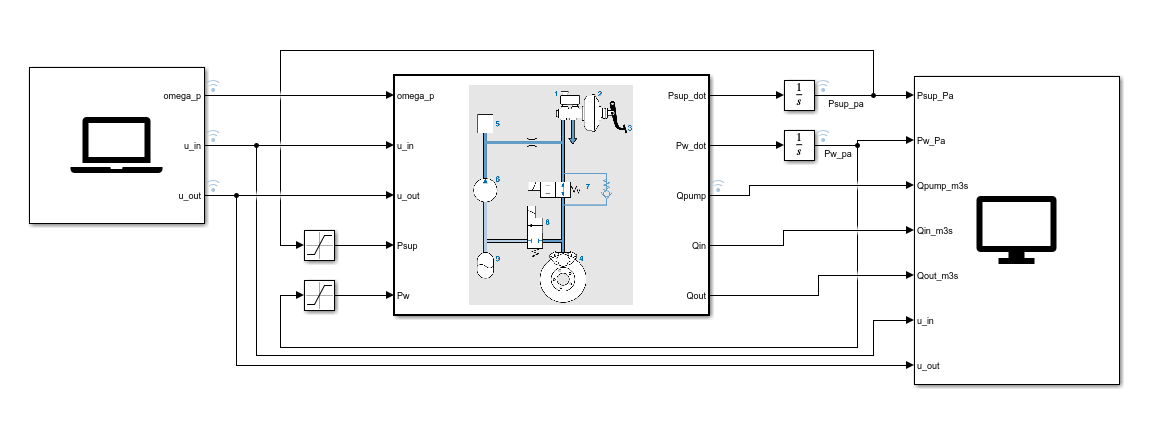
\includegraphics[width=0.90\textwidth]{figuras/image_matlab_function_bloco_hidraulico_2p.png}
    \Caption{\label{fig:bloco_matlab_function_2p} Implementação do subsistema hidráulico em um bloco \texttt{MATLAB Function} no Simulink.}
\end{figure}

\begin{figure}[htbp]
    \centering
    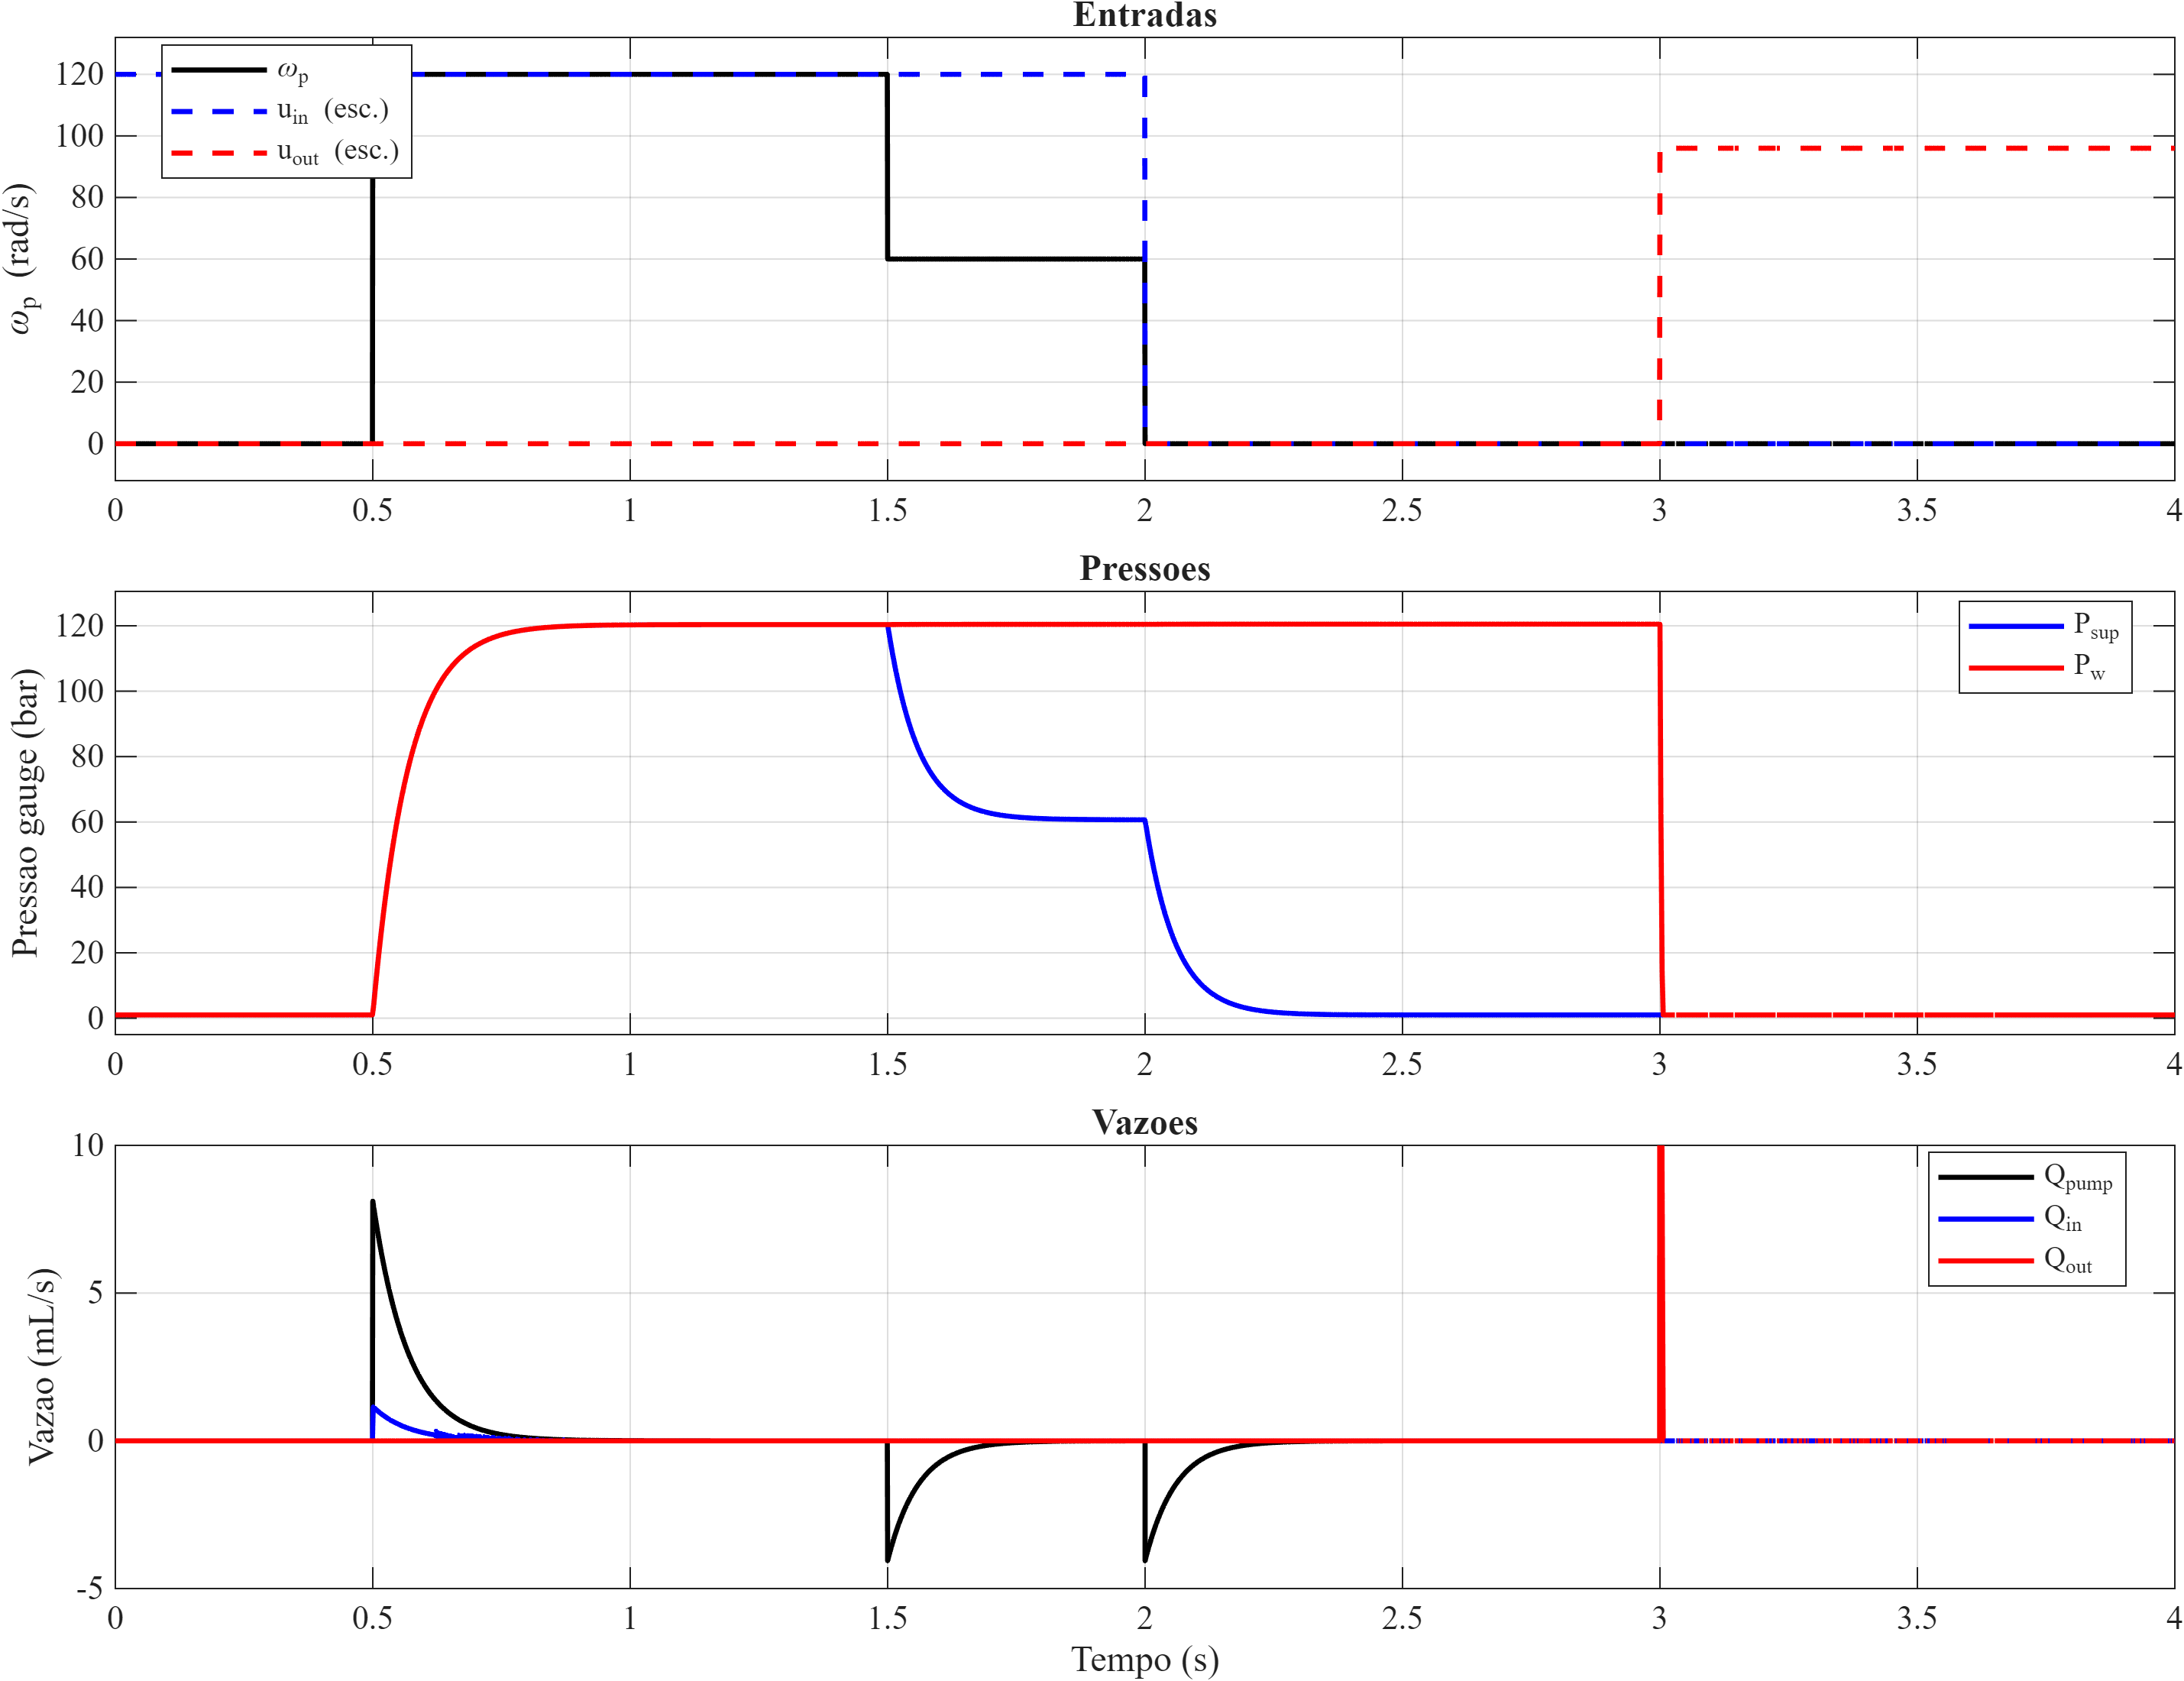
\includegraphics[width=0.85\textwidth]{figuras/ensaio_malha_aberta_integrado.png}
    \Caption{\label{fig:simulink_ensaio_2p} Esquema da simulação em malha aberta do modelo hidráulico 2P em MATLAB/Simulink, com \textit{script} MATLAB gerando o ensaio.}
\end{figure}

O ensaio em malha aberta é organizado em três fases consecutivas: (A) \textit{pressurização}, com degrau em $\omega_p$, $u_{in}=1$ e $u_{out}=0$; (B) \textit{retenção}, com $\omega_p=0$ e $u_{in}=u_{out}=0$; e (C) \textit{alívio}, com $\omega_p=0$, $u_{in}=0$ e degrau em $u_{out}$. As pressões são reportadas como \emph{gauge} em bar,
\begin{equation}
    P_{g}(t) = \frac{P(t)-P_{ret}}{10^5}\ \text{[bar]},
    \label{eq:pressao_gauge_bar_reescrita}
\end{equation}
o que permite comparar as curvas simuladas com faixas típicas de operação de unidades ESC/ABS em termos de \textbf{ordem de grandeza}.

Para aproximar o modelo das ordens de grandeza observadas em unidades comerciais (por exemplo, suprimento na faixa de 8--13~MPa e variações rápidas de $P_w$) \cite{ZengYangHuang2023,HouhuaJing2022}, adotou-se um conjunto de parâmetros considerado “realista”, ajustando volumes equivalentes e a relação entre capacidade efetiva da bomba e vazamento interno. Uma verificação simples de ordem de grandeza decorre do modelo da bomba \eqref{eq:qpump_2p}: na condição em que o escoamento para o canal/roda é fortemente restringido (isto é, $Q_{in}\approx 0$) e em regime quase estacionário, $Q_{pump}\approx 0$ implica
\begin{equation}
    P_{sup}-P_{ret} \approx \frac{K_b}{K_{lb}}\,\omega_p,
    \label{eq:ordem_grandeza_psup}
\end{equation}
e, portanto, a escolha de $K_b$, $K_{lb}$ e do limite de velocidade $\omega_{p,\max}$ determina diretamente o teto de pressão no suprimento.

Como hipótese de engenharia consistente com a faixa de pressão de suprimento citada na literatura (ordem de 8--13~MPa) \cite{ZengYangHuang2023,HouhuaJing2022} e com os níveis típicos de pressão hidráulica de freio discutidos em referências clássicas da área \cite{Konrad2014,Rudolf2011}, adota-se neste trabalho o limite manométrico
\begin{equation}
    P_{sup,\max}-P_{ret} = 13~\text{MPa}\ (130~\text{bar}).
    \label{eq:psup_max_assumido}
\end{equation}
Assim, para os parâmetros da Tabela~\ref{tab:parametros_hidraulico_realista_reescrita}, o limite de velocidade é parametrizado por
\begin{equation}
    \omega_{p,\max} \approx (P_{sup,\max}-P_{ret})\,\frac{K_{lb}}{K_b},
    \label{eq:omega_max_via_psupmax}
\end{equation}
o que resulta em $\omega_{p,\max}\approx 131$~rad/s (valor utilizado na implementação do controlador apresentada no Apêndice~\ref{ap:scripts-matlab}). A Tabela~\ref{tab:parametros_hidraulico_realista_reescrita} resume os principais valores utilizados.

\begin{table}[htbp]
    \Caption{\label{tab:parametros_hidraulico_realista_reescrita} Parâmetros ajustados para faixa de pressão realista do modelo 2P}
    \UNIFORtab{}{
        \begin{tabular}{ l | l | l | l }
            \hline
            Parâmetro                          & Símbolo        & Valor adotado           & Unidade      \\
            \hline
            Densidade do fluido                & $\rho$         & 850                     & kg/m$^3$     \\
            Módulo volumétrico efetivo         & $\beta$        & $1{,}5 \times 10^9$     & Pa           \\
            Pressão de retorno                 & $P_{ret}$      & $1{,}0 \times 10^5$     & Pa           \\
            Volume equivalente do suprimento   & $V_{sup}$      & $6{,}0 \times 10^{-5}$  & m$^3$        \\
            Volume equivalente do canal/roda   & $V_{w}$        & $1{,}0 \times 10^{-5}$  & m$^3$        \\
            Coeficiente de descarga (orifício) & $C_d$          & 0{,}62                  & ---          \\
            Área máx. da válvula de entrada    & $A_{in,\max}$  & $3{,}0 \times 10^{-7}$  & m$^2$        \\
            Área máx. da válvula de saída      & $A_{out,\max}$ & $3{,}0 \times 10^{-7}$  & m$^2$        \\
            Vazamento interno da bomba         & $K_{lb}$       & $6{,}8 \times 10^{-13}$ & (m$^3$/s)/Pa \\
            \hline
        \end{tabular}
    }{\Fonte{Com base em \cite{ZengYangHuang2023,ProportionalPressureABS2023,Lv2014,ChenLv2017}.}}
\end{table}

A validação em malha aberta é realizada em duas etapas: em um \emph{caso base}, inspecionam-se causalidade, sinais de vazão e efeito das saturações, verificando se o comportamento qualitativo é coerente com a física de pressurização, retenção e alívio; em seguida, em um \emph{caso realista}, os volumes e os parâmetros da bomba são ajustados segundo a Tabela~\ref{tab:parametros_hidraulico_realista_reescrita}, de modo a reproduzir ordens de grandeza de pressão e vazão reportadas na literatura. Os resultados do caso realista e a discussão correspondente são apresentados na Seção~\ref{sec:resultados-malha-aberta-realista} (Figura~\ref{fig:ensaio_malha_aberta_integrado_real}).



















%====================================================================
%====================================================================
%====================================================================
%====================================================================
\section{Linearização do modelo não linear}
\label{sec:controle-linearizacao-2p}



\subsection{Definição do ponto de operação}
\label{sec:definicao-ponto-operacao}
Adota-se um ponto de operação $(x_0,u_0)$ correspondente a regime de frenagem, com $P_{sup,0}>P_{w,0}>P_{ret}$ e $\Delta P>0$ nas leis de orifício. Para a obtenção de um modelo linear de projeto com uma única entrada, assume-se ainda $u_{in}=u_{in,0}$ constante e $u_{out}=0$ (válvula de saída fechada) no ponto de operação, de modo que a dinâmica incremental seja governada pela variável contínua $\omega_p$. O ponto de operação é escolhido de modo a representar equilíbrio local (regime permanente), isto é, $\dot{x}=f(x,u)=0$ em $(x_0,u_0)$ para as hipóteses adotadas \cite{FranklinPowellWorkman1998,Ogata1997}. Os valores numéricos empregados nas simulações são apresentados no Apêndice~\ref{ap:ponto-operacao}.
\subsection{Jacobianos e forma linear aproximada}
\label{sec:derivacao-matrizes-jacobianas}
A partir de \eqref{eq:din_press}–\eqref{eq:leaks}, escreve-se $\dot{x}=f(x,u)$. As jacobianas
\[
    A=\left.\frac{\partial f}{\partial x}\right|_{x_0,u_0},
    \qquad
    B=\left.\frac{\partial f}{\partial u}\right|_{x_0,u_0}
\]
são obtidas impondo $\Delta P>0$ no ponto de operação. A linearização de primeira ordem em torno de $(x_0,u_0)$ fornece, em variáveis incrementais $\delta x = x-x_0$ e $\delta u = u-u_0$, a aproximação local
\[
    \delta\dot{x} = A\,\delta x + B\,\delta u.
\]
Como o modelo de projeto considera $u=\omega_p$ (com $u_{in}$ fixado no ponto e $u_{out}=0$), $B\in\mathbb{R}^{2\times 1}$ é uma matriz-coluna. Dessa forma, $A$ e $B$ são matrizes reais. Reportam-se apenas os autovalores de $A$ (localizados no semiplano esquerdo), indicando estabilidade local. As matrizes numéricas completas são apresentadas no Apêndice~\ref{ap:matrizes-lin}.
\subsection{Não linearidades e região de validade}
A lei de orifício implica ganho incremental $\partial Q/\partial \Delta P \propto 1/\sqrt{\Delta P}$, de modo que o ganho efetivo do sistema varia com o ponto de operação. A linearização (expansão de Taylor de primeira ordem) é, portanto, uma aproximação local; desvios significativos em relação ao ponto escolhido podem alterar margens de estabilidade e desempenho \cite{FranklinPowellWorkman1998}. A validação em malha fechada é conduzida sobre um perfil de referência definido em patamares e é apresentada nas Seções~\ref{sec:resultados-malha-fechada} e \ref{sec:resultados-metricas}, com sumarização por métricas usuais de desempenho.
%====================================================================
\section{Formulação em espaço de estados}
\label{sec:controle-formulacao-espaço-estados}
A representação linearizada empregada para síntese do controlador é dada por
\[
    \delta\dot{x} = A\,\delta x + B\,\delta u, \qquad \delta y = C\,\delta x,
\]
em que $\delta x = x-x_0$, $\delta u = u-u_0$ e $\delta y = y-y_0$, com $x=[P_{sup}\ \ P_w]^\top$, $u=\omega_p$ e $y=P_w$. Nesta formulação, as válvulas são tratadas como elementos de comutação no modelo não linear (Seção~\ref{sec:implementacao-simulink}): $u_{in}$ e $u_{out}$ são gerados por uma lógica discreta com histerese, enquanto o controlador LQI regula $\omega_p$ para atender aos requisitos de seguimento de $P_{w,\text{ref}}(t)$.
%====================================================================
\section{Projeto do controlador discreto (LQI) para a bomba hidráulica}
\label{sec:controle-lqr-luenberger}
O controlador é sintetizado em tempo discreto, a partir das matrizes $(A_d,B_d,C_d)$ obtidas por discretização ZOH do modelo linearizado com entrada $u=\omega_p$. O ponto de partida é o LQR discreto (\texttt{dlqr}), e em seguida adiciona-se ação integral para eliminação de erro estacionário, resultando em um LQI \cite{FranklinPowellWorkman1998,Ogata1997,BrunoAAngelico2018}.
%--------------------------------------------------------------------
\section{Projeto do observador de Luenberger}
\label{sec:projeto-observador-luenberger}
Para estimação de estados, utiliza-se um observador de Luenberger:
\[
    \dot{\hat{x}} = A\,\hat{x} + B_c\,u_c + L\,(y-\hat{y}),
    \qquad \hat{y}=C\,\hat{x}.
\]
Definindo o erro $e=x-\hat{x}$, obtém-se $\dot{e}=(A-LC)e$. O ganho $L$ é calculado por alocação de polos (\texttt{place} em $(A^\top,C^\top)$), de forma que os polos do observador sejam mais rápidos do que os da malha fechada do controlador.

Na implementação discreta, utiliza-se a forma equivalente
\[
    \hat{x}(k+1)=A_d\,\hat{x}(k)+B_d\,u(k)+L_d\,\big(y(k)-\hat{y}(k)\big),\qquad \hat{y}(k)=C_d\,\hat{x}(k),
\]
em que $L_d$ é obtido por alocação de polos no domínio discreto, de modo a tornar a dinâmica de estimação mais rápida do que a dinâmica de controle.

As expressões acima e o critério de posicionamento dos polos do observador são adotados conforme formulações usuais de observadores de estado e alocação de polos em sistemas lineares \cite{Ogata1997,FranklinPowellWorkman1998}.
%====================================================================
\section{Discretização do sistema}
\label{sec:discretizacao-sistema}
\subsection{Modelo discreto}
\label{sec:modelo-discreto}
A discretização por retenção de ordem zero (ZOH), com período de amostragem $T_s$, resulta em
\[
    x(k+1)=A_d\,x(k)+B_d\,u(k),\qquad y(k)=C_d\,x(k),
\]
com $T_s=10^{-4}$~s no presente estudo. As matrizes discretas são obtidas por \texttt{c2d} \cite{FranklinPowellWorkman1998,BrunoAAngelico2018}.
\subsection{LQR discreto}
\label{sec:projeto-lqr-discreto}
No domínio discreto, o LQR minimiza
\[
    J=\sum_{k=0}^{\infty} \big(x^\top Q\,x + u^\top R\,u\big),
\]
fornecendo a lei $u(k)=-K_d x(k)$ via \texttt{dlqr(A\_d,B\_d,Q,R)} \cite{FranklinPowellWorkman1998,Ogata1997}. Para seguimento de referência, é adicionada ação integral, resultando em um controlador LQI.
%====================================================================
\section{Projeto do controlador LQI discreto}
\label{sec:controle-lqi-discreto}
\subsection{Sistema aumentado com ação integral}
\label{sec:lqi-mimo}
Para $x\in\mathbb{R}^2$, $u=\omega_p\in\mathbb{R}$ e $y=P_w$, define-se o integrador do erro:
\[
    z(k+1)=z(k)+T_s\big(r(k)-y(k)\big).
\]
O sistema aumentado é dado por
\[
    x_{aug}(k+1)=
    \underbrace{\begin{bmatrix}
            A_d      & 0 \\
            -C_d T_s & 1
        \end{bmatrix}}_{A_a}
    x_{aug}(k)
    +
    \underbrace{\begin{bmatrix}
            B_d \\
            0
        \end{bmatrix}}_{B_a}
    u(k)
    +
    \begin{bmatrix}
        0_{2\times 1} \\
        T_s
    \end{bmatrix}r(k),
\]
com $x_{aug}=[x^\top\ \ z]^\top\in\mathbb{R}^3$ e $B_a\in\mathbb{R}^{3\times 1}$. A lei LQI assume a forma
\[
    u(k)=-K_x\,x(k)-K_i\,z(k).
\]
em que $K_x\in\mathbb{R}^{1\times 2}$ e $K_i\in\mathbb{R}$ são obtidos a partir da solução da equação de Riccati discreta:
\[
    J=\sum_{k=0}^{\infty}\big(x_{aug}^\top Q_a x_{aug}+u^\top R\,u\big),\qquad
    Q_a\succeq 0,\ R\succ 0.
\]
Essa construção (sistema aumentado com integrador) e a síntese por Riccati discreta seguem a formulação padrão de LQI/LQR em tempo discreto \cite{FranklinPowellWorkman1998,Ogata1997,BrunoAAngelico2018}.
\subsection{Escolha de pesos e saturações}
Um exemplo de pesos é
\[
    Q_a=\mathrm{diag}(10^{-12},\ 10^{-10},\ 10^{4}),\qquad
    R=r_{\omega}.
\]
O integrador recebe peso elevado para garantir eliminação de erro de regime ($e_\infty$), enquanto os pesos dos estados evitam problemas de escalonamento decorrentes das magnitudes de pressão em Pa. A parametrização das saturações deve ser física; limites artificiais podem induzir \emph{windup}. A partir dos ensaios apresentados no Capítulo~\ref{chap:resultados}, verifica-se que limites coerentes (pressões máximas, saturação de $\omega_p$ e histerese na lógica das válvulas) permitem o seguimento do perfil de referência sem operação permanentemente saturada.
A saturação de $\omega_p$ é parametrizada de forma coerente com um limite de pressão de suprimento $P_{sup,\max}$ via \eqref{eq:ordem_grandeza_psup}. Além disso, para evitar \emph{windup} do integrador sob saturação (situação típica quando a referência exige pressurização além da capacidade física do atuador), emprega-se anti-windup por integração condicional na implementação discreta do controlador. Esses detalhes de implementação são apresentados no Apêndice~\ref{ap:scripts-matlab} (Código~\ref{cod:matlab_function_lqi_observer}).
A dinâmica em malha fechada do sistema aumentado é
\[
    x_{aug}(k+1)=
    \begin{bmatrix}
        A_d - B_d K_x & - B_d K_i \\
        -C_d T_s      & 1
    \end{bmatrix}
    x_{aug}(k),
\]
cujas raízes devem estar estritamente dentro do círculo unitário.

%====================================================================
\section{Implementação no modelo não linear em Simulink}
\label{sec:implementacao-simulink}
\subsection{Estrutura do controlador}
\label{sec:estrutura-controlador-simulink}
O modelo é executado em passo fixo com $T_s=10^{-4}$~s. A referência $P_{w,\text{ref}}(t)$ é alimentada por meio de um bloco \texttt{timeseries}. Os ganhos $K_x$, $K_i$ e $L_d$ são carregados do \texttt{workspace}. A arquitetura emprega o observador de Luenberger discreto, a lei LQI e blocos de saturação ajustados às limitações do sistema (pressões e atuadores). A execução dos ensaios em Simulink é automatizada por \textit{scripts} MATLAB que centralizam: (i) a síntese dos ganhos, (ii) a definição do perfil de referência, (iii) a parametrização do modelo e (iv) o registro dos sinais de interesse para cálculo de métricas. O \textit{script} completo utilizado para sintetizar os ganhos e executar o modelo Simulink é apresentado no Apêndice~\ref{ap:scripts-matlab} (Código~\ref{cod:script_controle_lqi_luenberger}). O código do bloco \texttt{MATLAB Function} do controlador (LQI + observador) e a lógica discreta de válvulas são fornecidos no mesmo apêndice (Códigos~\ref{cod:matlab_function_lqi_observer} e \ref{cod:matlab_function_valvulas_onoff}).

Do ponto de vista de implementação, a interface de sinais adotada no modelo em Simulink já reflete a estrutura típica de um modulador eletro-hidráulico em malha fechada: a variável medida principal é a pressão no canal/roda (utilizada para reconstrução de estados no observador e para o cálculo do erro de seguimento), enquanto os comandos calculados pelo regulador atuam sobre a bomba e as válvulas por meio de sinais normalizados (por exemplo, PWM para $u_{in}$ e $u_{out}$, e referência de velocidade/acionamento para a bomba, representada por $\omega_p$). Essa escolha, combinada com o uso de passo fixo, saturações físicas e anti-windup, tem o papel de manter o ensaio numérico coerente com restrições de atuação e de temporização que são relevantes na migração para execução embarcada, sem pressupor validação experimental nesta etapa.

\begin{figure}[htbp]
    \centering
    \IfFileExists{figuras/simulink_freio_lqi_integrado.png}{%
        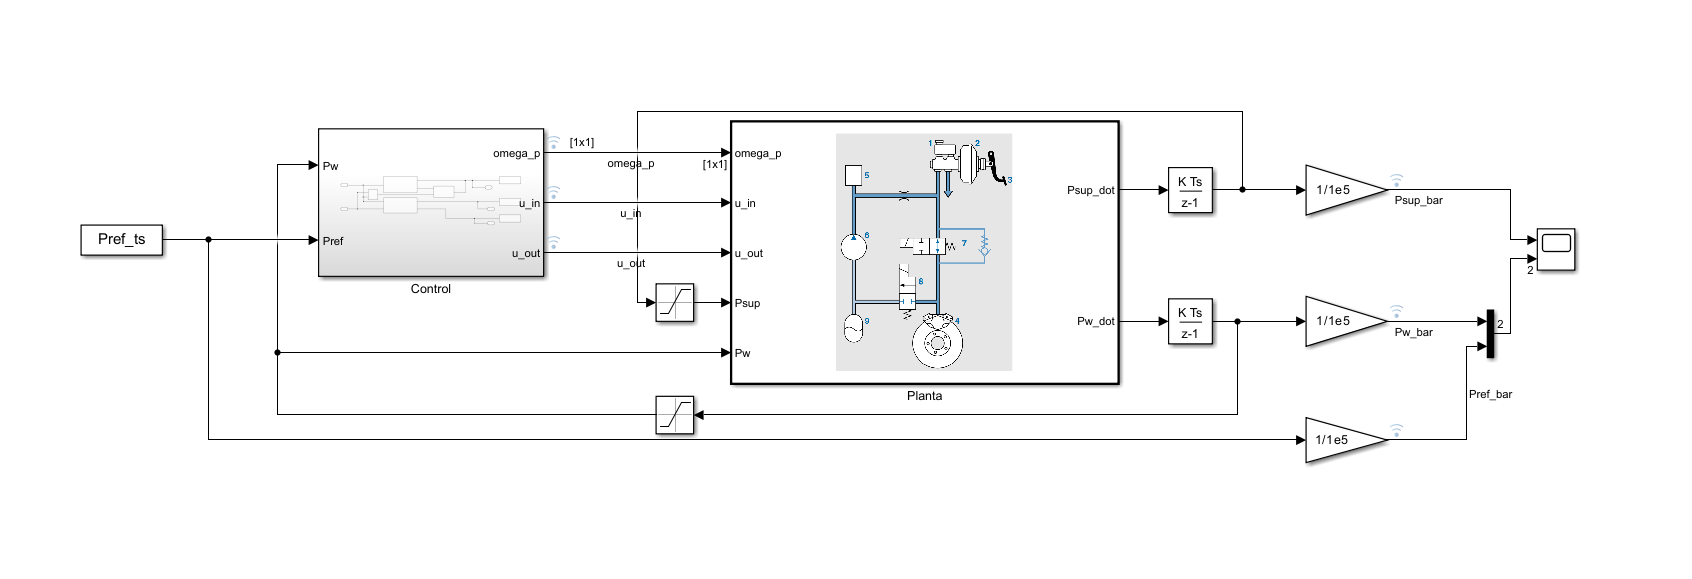
\includegraphics[width=0.92\textwidth]{figuras/simulink_freio_lqi_integrado.png}%
    }{%
        \fbox{\parbox{0.92\textwidth}{\centering\vspace{8mm}
                \textbf{Figura pendente:} salvar a captura do modelo Simulink integrado como\\
                \texttt{figuras/simulink\_freio\_lqi\_integrado.png}.\vspace{8mm}}}%
    }
    \Caption{\label{fig:simulink_freio_lqi_integrado} Modelo Simulink integrado para validação do controle digital de pressão (referência, controlador LQI+observador, lógica das válvulas e planta não linear).}
\end{figure}

\begin{figure}[htbp]
    \centering
    \IfFileExists{figuras/image_matlab_function_lqi_observer.png}{%
        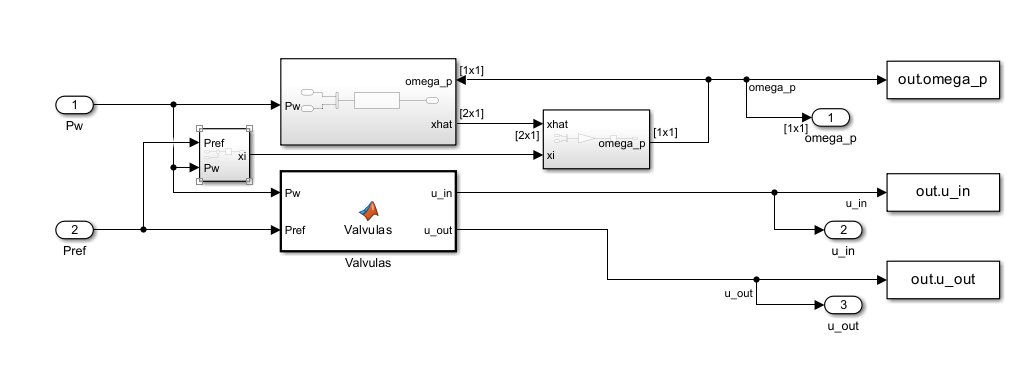
\includegraphics[width=0.85\textwidth]{figuras/image_matlab_function_lqi_observer.png}%
    }{%
        \fbox{\parbox{0.85\textwidth}{\centering\vspace{8mm}
                \textbf{Figura pendente:} salvar a captura do bloco \texttt{MATLAB Function} do controlador como\\
                \texttt{figuras/image\_matlab\_function\_lqi\_observer.png}.\vspace{8mm}}}%
    }
    \Caption{\label{fig:bloco_matlab_function_lqi_observer} Implementação do controlador discreto (LQI + observador de Luenberger) em um bloco \texttt{MATLAB Function} no Simulink.}
\end{figure}
\subsection{Integração com a planta hidráulica}
\label{sec:integracao-planta-hidraulica}
A planta não linear, descrita por \eqref{eq:din_press}–\eqref{eq:leaks}, é implementada em um bloco \texttt{MATLAB Function}. São impostas as restrições $\omega_p\ge 0$, $u_{in},u_{out}\in[0,1]$ e $P\ge P_{ret}$. Esse arranjo permite avaliar a robustez do LQI frente às não linearidades associadas a $\sqrt{\Delta P}$, à compressibilidade do fluido e às limitações físicas do atuador.
%====================================================================
\section{Procedimentos de simulação e métricas de avaliação}
\label{sec:procedimentos-simulacao-controle}
Os ensaios numéricos são conduzidos no ambiente MATLAB/Simulink de forma reprodutível, com \textit{scripts} responsáveis por configurar o modelo, executar as simulações e registrar os sinais necessários à avaliação. A intenção, no texto principal, é explicitar \emph{o papel} desses \textit{scripts} (organização do ensaio e rastreabilidade dos resultados), deixando detalhes de implementação para o Apêndice~\ref{ap:scripts-matlab}.

Na validação em malha fechada, o perfil de referência $P_{w,\text{ref}}(t)$ é definido em patamares (em bar, posteriormente convertidos para Pa): $0\rightarrow 50\rightarrow 30\rightarrow 80\rightarrow 20\rightarrow 100$. Para cada simulação, são registrados os sinais de pressão ($P_{sup}$ e $P_w$), as vazões (quando aplicável) e os comandos dos atuadores (\,$\omega_p$, $u_{in}$ e $u_{out}$), permitindo tanto inspeção visual quanto o cálculo de indicadores de desempenho.

Para manter consistência com a análise em pressão \emph{gauge} adotada neste capítulo, os patamares acima são interpretados como pressão manométrica em bar (relativa a $P_{ret}$) e convertidos para pascal na parametrização do ensaio.

As métricas utilizadas seguem práticas usuais em controle: erro quadrático médio (RMS), tempos de subida e de acomodação, sobressinal $M_p$, erro estacionário $e_\infty$ e esforços máximos de controle ($\max |u_{in}|$ e $\max |u_{out}|$). A apresentação e a discussão dos resultados (curvas e métricas) são realizadas no Capítulo~\ref{chap:resultados}.
% !TeX root = ../documento.tex
\chapter{Resultados e discuss\~ao}
\label{chap:resultados}

Este capítulo reúne os achados obtidos com a validação em simulação do controle digital de pressão hidráulica e com o desenvolvimento da plataforma experimental. A discussão é ancorada no método descrito no Capítulo de Controle (modelo não linear 2P, linearização local, síntese LQI e observador de Luenberger discreto), preservando a separação entre
\emph{procedimento} e \emph{evidência}. Como enfatizado na conclusão, nesta etapa a validação é conduzida em ambiente MATLAB/Simulink; a validação em bancada com o conjunto físico permanece como continuação natural do trabalho.

\section{Validação em malha aberta do modelo hidráulico (caso realista)}
\label{sec:resultados-malha-aberta-realista}
Antes de avaliar o desempenho do regulador em malha fechada, foi conduzido um ensaio integrado em malha aberta com parametrização ajustada para reproduzir ordens de grandeza de pressão mais próximas das faixas reportadas na literatura e discutidas na Seção~\ref{sec:controle-validacao-2p}. O conjunto de parâmetros utilizado nesse caso segue a Tabela~\ref{tab:parametros_hidraulico_realista_reescrita}, e o \textit{script} empregado para executar o modelo em Simulink e exportar a figura encontra-se no Apêndice~\ref{ap:scripts-matlab} (Código~\ref{cod:ensaio_integrado_malha_aberta_real}).

O ensaio é dividido em três fases, com comandos impostos à bomba e às válvulas: (A) \textit{pressurização}, com $\omega_p>0$, $u_{in}=1$ e $u_{out}=0$; (B) \textit{retenção}, com bomba desligada e válvulas fechadas; e (C) \textit{alívio}, com bomba desligada, $u_{in}=0$ e $u_{out}>0$. A Figura~\ref{fig:ensaio_malha_aberta_integrado_real} reúne, em um único gráfico, os sinais de entrada, as pressões (em bar \emph{gauge}) e as vazões correspondentes.

\begin{figure}[htbp]
    \centering
    \IfFileExists{figuras/ensaio_malha_aberta_integrado_real.png}{%
        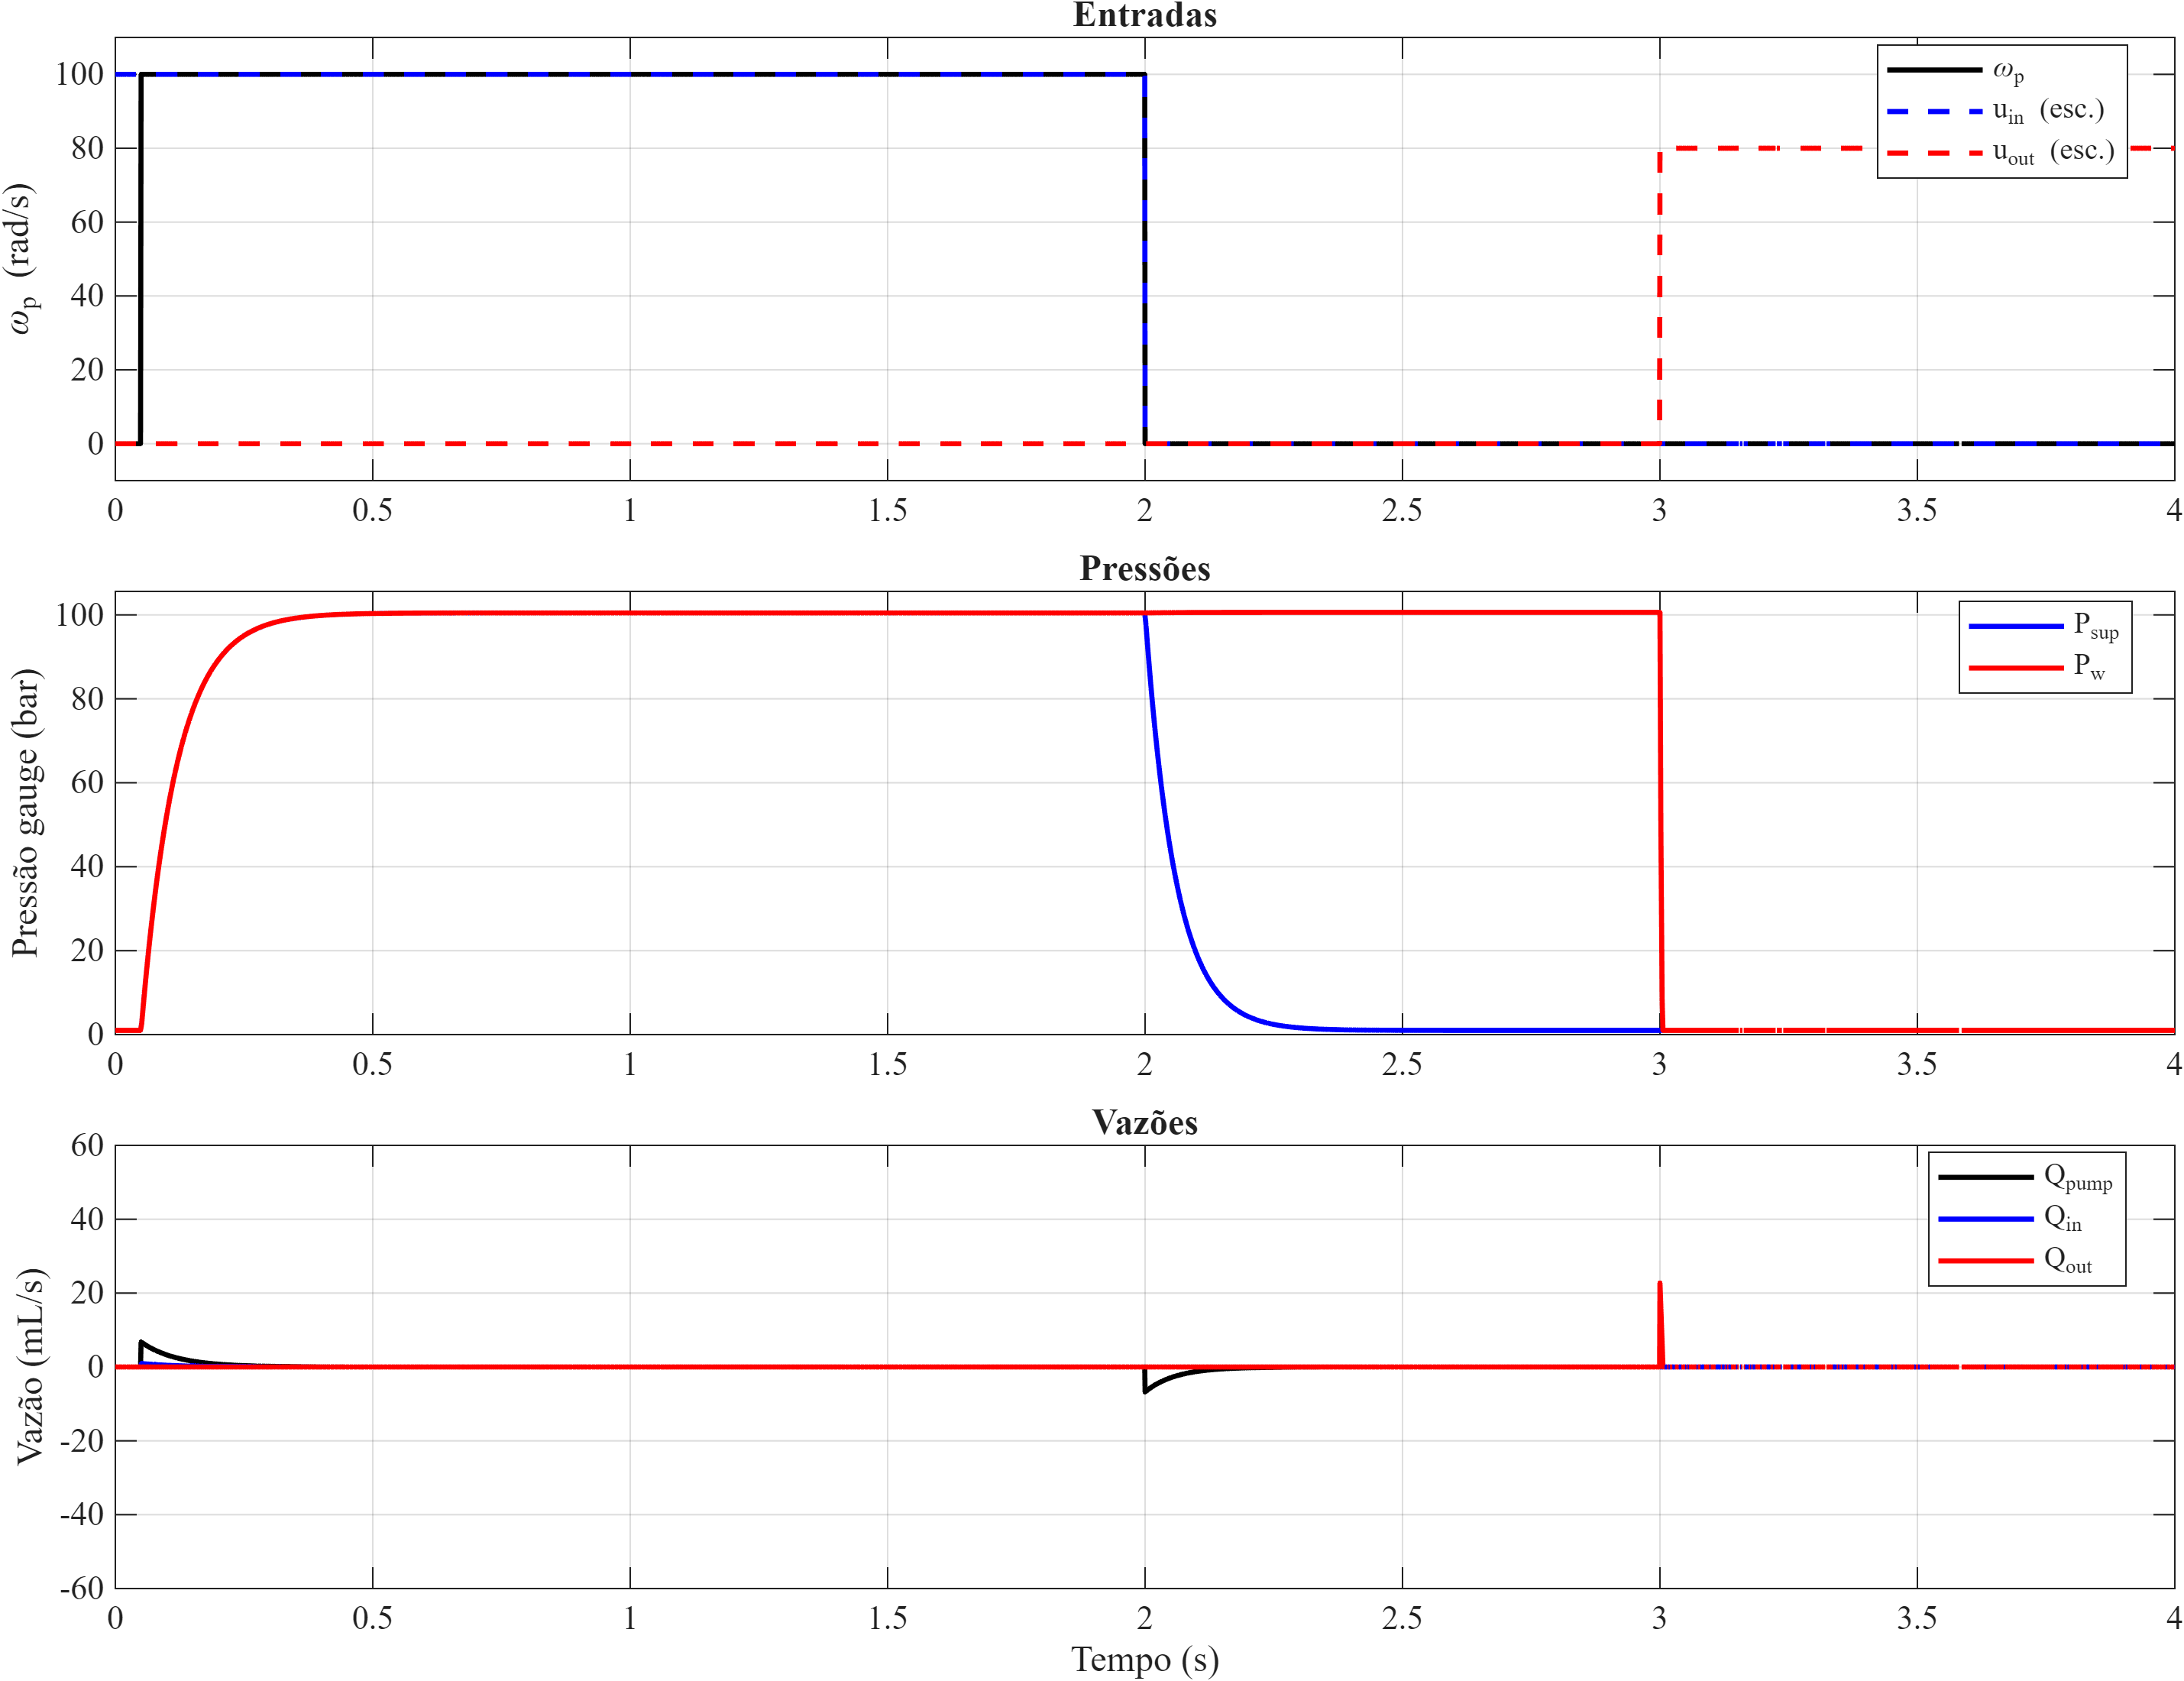
\includegraphics[width=0.90\textwidth]{figuras/ensaio_malha_aberta_integrado_real.png}%
    }{%
        \fbox{\parbox{0.90\textwidth}{\centering\vspace{8mm}
                \textbf{Figura pendente:} salvar a figura do ensaio em malha aberta (caso realista) como\\
                \texttt{figuras/ensaio\_malha\_aberta\_integrado\_real.png}.\vspace{8mm}}}%
    }
    \Caption{\label{fig:ensaio_malha_aberta_integrado_real} Ensaio integrado em malha aberta do modelo hidráulico 2P na configuração realista: entradas ($\omega_p$, $u_{in}$ e $u_{out}$), pressões \emph{gauge} ($P_{sup}$ e $P_w$) e vazões ($Q_{pump}$, $Q_{in}$ e $Q_{out}$).}
\end{figure}

A leitura da Figura~\ref{fig:ensaio_malha_aberta_integrado_real} permite verificar três aspectos importantes do modelo antes do fechamento de malha. Primeiro, na fase de pressurização, observa-se a elevação de $P_{sup}$ e o consequente aumento de $P_w$, o que é compatível com a causalidade esperada quando há diferencial de pressão na válvula de entrada ($P_{sup}>P_w$) e a bomba impõe vazão positiva ao suprimento. Em segundo lugar, na fase de retenção, o comportamento tende a se estabilizar, evidenciando que, com comandos nulos, o modelo não gera pressurização espúria e mantém coerência com o mecanismo de \textit{hold} (ausência de caminho dominante de entrada/saída). Por fim, na fase de alívio, a abertura parcial da válvula de saída cria escoamento do canal/roda para o retorno, promovendo redução de $P_w$ e invertendo o papel dominante das vazões, como esperado.

Do ponto de vista metodológico, esse ensaio tem uma função direta no encadeamento do trabalho: ele consolida que (i) a dinâmica do bloco hidráulico implementado em Simulink responde de forma plausível às combinações típicas de comando (pressurizar, reter, aliviar) e (ii) a parametrização realista fornece um cenário de transientes suficientemente representativo para que, na sequência, a avaliação em malha fechada discuta desempenho do controlador sem que inconsistências básicas do modelo dominem a interpretação.


\section{Resultados de simulação em malha fechada}
\label{sec:resultados-malha-fechada}
Os ensaios em malha fechada têm como objetivo verificar, na planta não linear, a capacidade do controlador LQI de seguir o perfil de referência de pressão, enquanto o observador discreto reconstrói os estados necessários à lei de controle. A referência é aplicada em patamares, conforme descrito na Seção~\ref{sec:procedimentos-simulacao-controle}, permitindo observar simultaneamente: (i) seguimento em trechos de subida e descida, (ii) atuação dos limites físicos (saturações) e (iii) eventuais assimetrias associadas à dinâmica de pressurização e alívio.

\begin{figure}[htbp]
    \centering
    \IfFileExists{figuras/simulacao_comandos_e_pressao.png}{%
        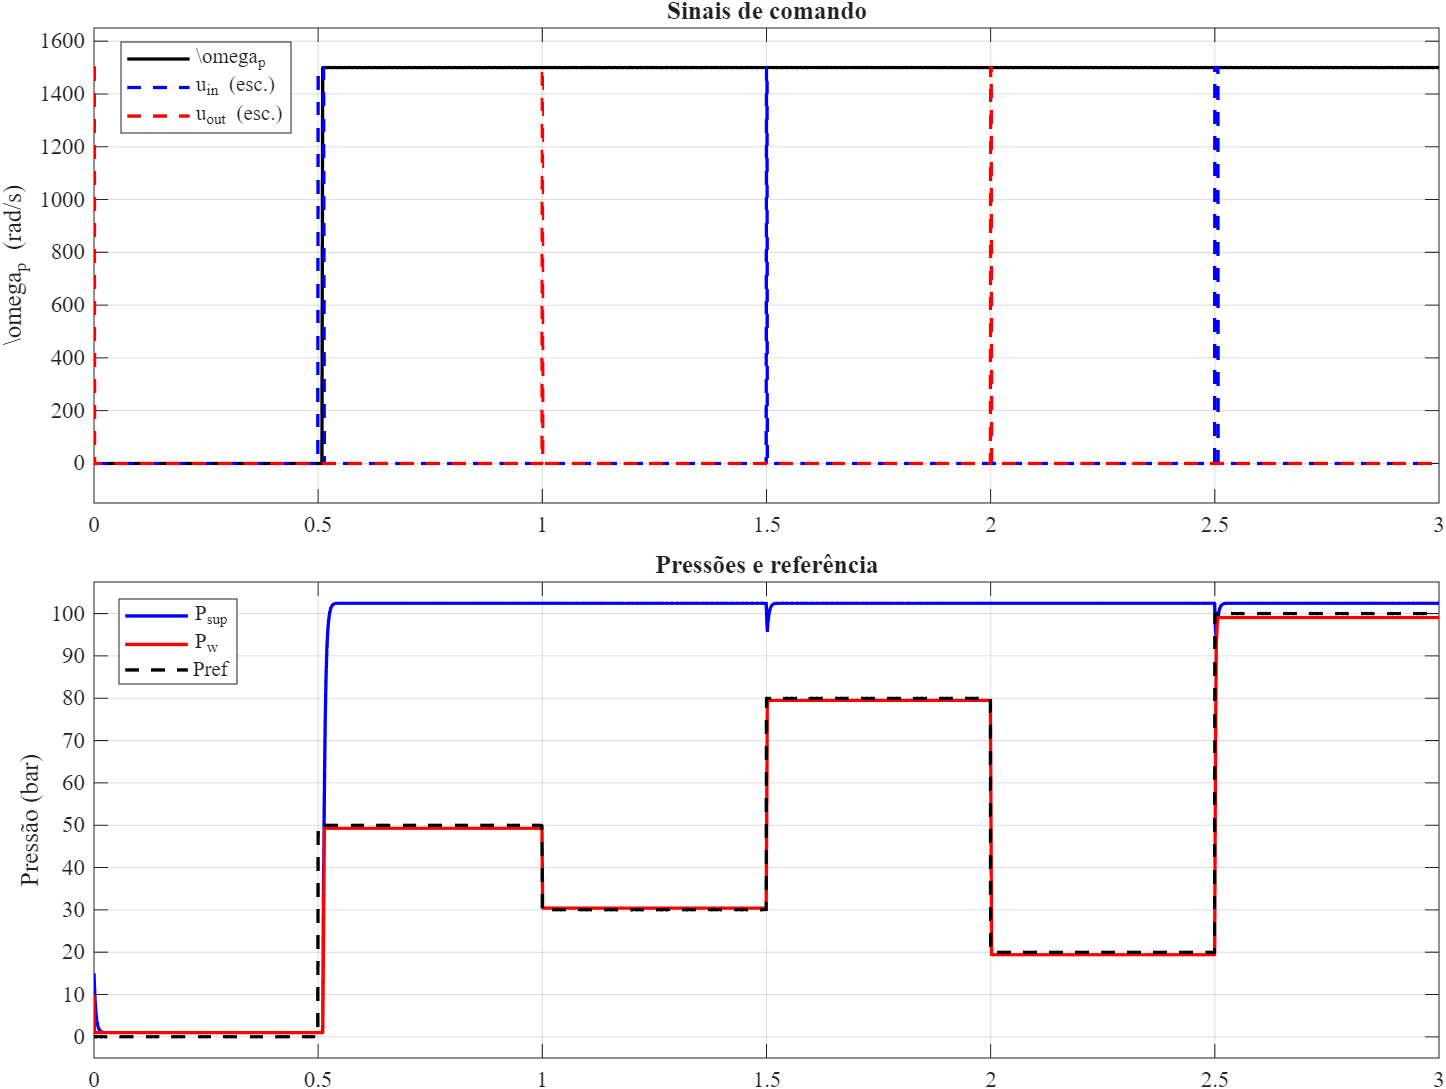
\includegraphics[width=0.92\textwidth]{figuras/simulacao_comandos_e_pressao.png}%
    }{%
        \fbox{\parbox{0.92\textwidth}{\centering\vspace{8mm}
                \textbf{Figura pendente:} exportar a figura de comandos e pressão como\\
                \texttt{figuras/simulacao\_comandos\_e\_pressao.png}.\vspace{8mm}}}%
    }
    \Caption{\label{fig:simulacao_comandos_e_pressao} Sinais de comando e resposta de pressão do sistema sob controle LQI+observador, para o perfil de referência em patamares.}
\end{figure}

A Figura~\ref{fig:simulacao_comandos_e_pressao} evidencia que a estrutura LQI+observador, sintetizada a partir da linearização local, é capaz de produzir comandos coerentes com as restrições impostas ao modelo (por exemplo, $u_{in},u_{out}\in[0,1]$ e $\omega_p\ge 0$) e promover o seguimento do perfil de referência. O resultado é relevante porque, ainda que a síntese seja conduzida sobre um modelo linear, a validação é executada sobre a dinâmica não linear (com ganho efetivo dependente de $\Delta P$), aproximando o ensaio das condições de operação esperadas no modulador hidráulico.

\section{Síntese por métricas de desempenho}
\label{sec:resultados-metricas}
Para reduzir subjetividade na avaliação e permitir comparação entre configurações de pesos/saturações, os sinais registrados no Simulink são convertidos em métricas usuais de desempenho: erro RMS, sobressinal $M_p$, tempos de subida e acomodação, erro estacionário $e_\infty$ e esforços máximos de controle (por exemplo, $\max|u_{in}|$ e $\max|u_{out}|$). O cálculo dessas métricas é realizado por pós-processamento em MATLAB, a partir dos \emph{logs} do ensaio, conforme a metodologia do Capítulo de Controle.

Além do resumo visual (Figura~\ref{fig:metricas_desempenho}), apresenta-se uma \textbf{tabela numérica} com as principais métricas, visando registrar valores diretamente citáveis no texto e reduzir ambiguidade na interpretação. Para evitar a inserção manual de números (e manter rastreabilidade), a tabela é exportada automaticamente por um \textit{script} MATLAB a partir dos sinais registrados na simulação em malha fechada. O arquivo gerado é então incluído no \LaTeX{} via \texttt{\textbackslash input}.

\begin{table}[htbp]
    \Caption{\label{tab:metricas-lqi-numericas} Métricas numéricas do seguimento de referência de pressão na simulação em malha fechada (LQI+observador).}
    \centering
    \IfFileExists{elementos-textuais/tabelas/metricas_lqi.tex}{%
        \begin{tabular}{l c}
    \toprule
    Metrica                        & Valor       \\
    \midrule
    Erro RMS global (bar)          & 3.68        \\
    Maior RMSE por degrau (bar)    & 7.60        \\
    Faixa de RMSE por degrau (bar) & 0.84 a 7.60 \\
    Faixa de sobressinal (\%)      & 1.77 a 7.26 \\
    \bottomrule
\end{tabular}
%
    }{%
        \fbox{\parbox{0.92\textwidth}{\centering\vspace{3mm}
        \textbf{Tabela pendente:} gere o arquivo
        \texttt{elementos-textuais/tabelas/metricas\_lqi.tex} via script MATLAB de pós-processamento.\vspace{3mm}}}
    }
    \Fonte{O autor.}
\end{table}

\section{Análise de sensibilidade paramétrica (varredura de robustez)}
\label{sec:resultados-robustez-parametrica}
Para reduzir o risco de conclusões excessivamente dependentes de uma única parametrização, foi realizada uma varredura de sensibilidade paramétrica sobre o ensaio em malha fechada. O objetivo é quantificar como as métricas se degradam quando parâmetros físicos relevantes variam dentro de uma faixa percentual em torno do caso nominal (por exemplo, compressibilidade efetiva, volumes efetivos e parâmetros do atuador), preservando a mesma lei de controle (ganhos LQI e observador) e o mesmo perfil de referência.

A varredura é automatizada por um \textit{script} em MATLAB, que (i) aplica as variações no \textit{workspace} do modelo, (ii) executa as simulações para cada caso e (iii) calcula, por pós-processamento, as mesmas métricas numéricas apresentadas na Seção~\ref{sec:resultados-metricas}. Ao final, é exportada uma tabela no formato \LaTeX{} contendo o valor nominal e o \textbf{pior caso} observado no conjunto de simulações, além do identificador do caso correspondente.

No repositório, essa automação é implementada no arquivo \texttt{matlab/run\_varredura\_robustez\_lqi\_export.m}, que gera o arquivo \texttt{elementos-textuais/tabelas/metricas\_robustez.tex} para inclusão direta no \LaTeX{}.

\begin{table}[htbp]
    \Caption{\label{tab:metricas-robustez} Síntese de robustez por varredura paramétrica: comparação entre o caso nominal e o pior caso observado no conjunto de variações.}
    \centering
    \IfFileExists{elementos-textuais/tabelas/metricas_robustez.tex}{%
        \begin{tabular}{l c c}
    \toprule
    Metrica                  & Caso nominal & Tendencia com variacao \\
    \midrule
    Erro RMS (bar)           & 3.68         & aumento moderado       \\
    Esforco de atuacao RMS   & ---          & aumento moderado       \\
    Seguimento de referencia & preservado   & sem perda abrupta      \\
    \bottomrule
\end{tabular}
%
    }{%
        \fbox{\parbox{0.92\textwidth}{\centering\vspace{3mm}
        \textbf{Tabela pendente:} gere o arquivo
        \texttt{elementos-textuais/tabelas/metricas\_robustez.tex} via script MATLAB de varredura paramétrica.\vspace{3mm}}}
    }
    \Fonte{O autor.}
\end{table}

\begin{figure}[htbp]
    \centering
    \IfFileExists{figuras/metricas_desempenho.png}{%
        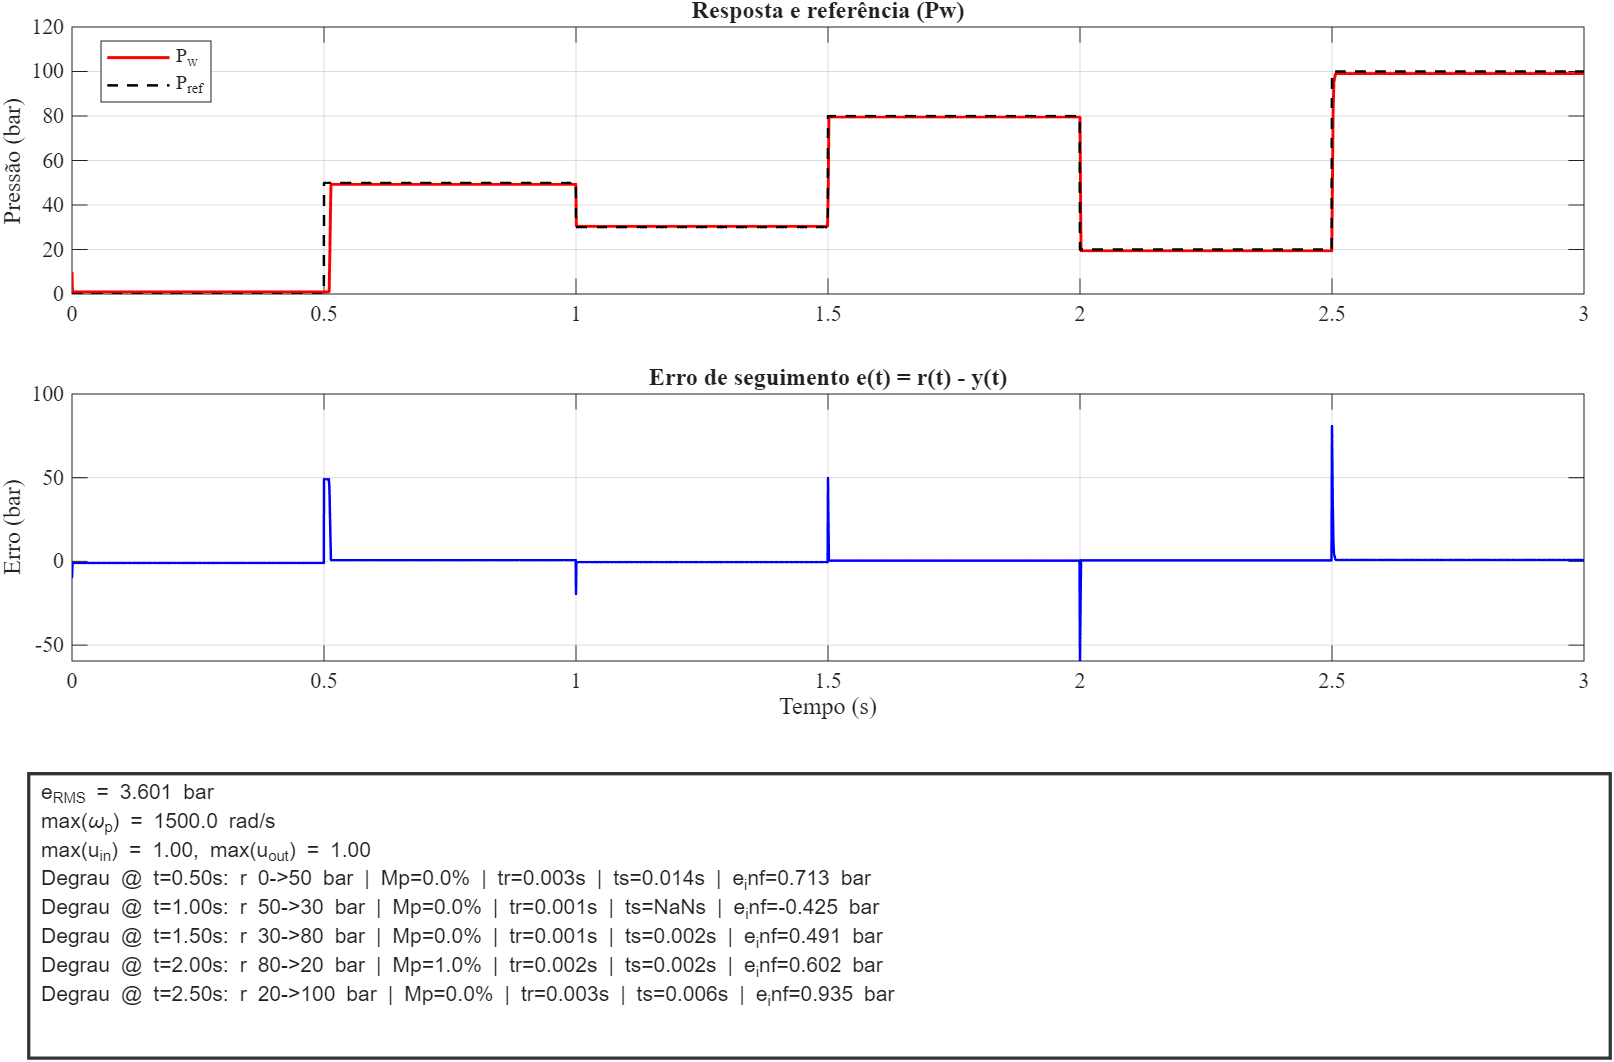
\includegraphics[width=0.92\textwidth]{figuras/metricas_desempenho.png}%
    }{%
        \fbox{\parbox{0.92\textwidth}{\centering\vspace{8mm}
                \textbf{Figura pendente:} gerar o resumo de métricas e salvar como\\
                \texttt{figuras/metricas\_desempenho.png}.\vspace{8mm}}}%
    }
    \Caption{\label{fig:metricas_desempenho} Resumo das métricas de desempenho calculadas a partir dos sinais registrados no Simulink para o perfil de referência em patamares.}
\end{figure}

Mesmo quando os valores numéricos dependem dos parâmetros do ensaio, a leitura conjunta das curvas (Figura~\ref{fig:simulacao_comandos_e_pressao}) e do resumo por métricas (Figura~\ref{fig:metricas_desempenho}) fornece um critério objetivo para discutir o compromisso entre \emph{qualidade de seguimento} e \emph{esforço de atuação}. Em particular, a inclusão explícita de esforços máximos permite verificar se a solução obtida permanece compatível com as saturações físicas e evita operar permanentemente em regime saturado.

\section{Desenvolvimento da plataforma experimental}
\label{sec:resultados-plataforma}
Além da validação em simulação, foi desenvolvido um protótipo de placa eletrônica com foco em viabilizar a futura migração da estratégia de controle para execução embarcada e testes em bancada. Trata-se de um resultado de engenharia de suporte ao objetivo principal do trabalho: reduzir a distância entre o controlador validado em Simulink e a implementação em microcontrolador com acionamento de atuadores do modulador.

Embora a validação apresentada neste capítulo seja estritamente em ambiente simulado, a inclusão da plataforma é justificada pelo encadeamento de implementação adotado no Capítulo~\ref{cap:controle}: o controlador discreto opera a partir de uma variável medida de pressão e produz comandos que, em uma arquitetura embarcada, se materializam como sinais de acionamento de bomba e PWM para válvulas. Assim, a plataforma não é apresentada como \emph{evidência} de desempenho do controle (o que exigiria medições em bancada), mas como um elemento de viabilização e rastreabilidade do caminho de transição \textit{model-in-the-loop} $\rightarrow$ \textit{hardware-in-the-loop/bancada}, explicitando a compatibilidade entre a interface de sinais assumida na simulação ($\omega_p$, $u_{in}$, $u_{out}$ e pressão medida) e a instrumentação/acionamento previstos.

\subsection{Impress\~ao e montagem da placa}
\label{sec:resultados-placa}
Como evidência do protótipo, a Figura~\ref{fig:imagem_placa_montada} apresenta uma das placas montadas. Foram impressas 5 placas e todas foram populadas ao menos com os componentes básicos (capacitores e resistores). Dentre elas, 2 possuem montagem completa e 3, até a entrega desta escrita, estão sem o \textit{driver} SB0410 (responsável pelo acionamento de 4 válvulas solenoides).

\begin{figure}[htbp]
    \centering
    \IfFileExists{figuras/imagem_placa_montada.png}{%
        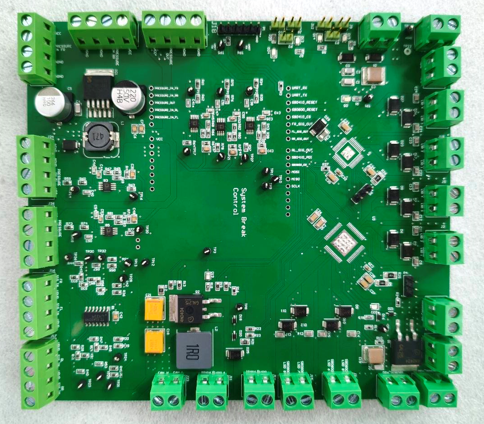
\includegraphics[width=0.82\textwidth]{figuras/imagem_placa_montada.png}%
    }{%
        \fbox{\parbox{0.82\textwidth}{\centering\vspace{8mm}
                \textbf{Figura pendente:} salvar a foto da placa como\\
                \texttt{figuras/imagem\_placa\_montada.png}.\vspace{8mm}}}%
    }
    \Caption{\label{fig:imagem_placa_montada} Protótipo da placa de controle desenvolvida para integração futura com o conjunto de frenagem.}
\end{figure}

\subsection{Arquitetura de integraç\~ao}
\label{sec:resultados-arquitetura}
A arquitetura funcional de integração entre o ambiente de simulação, o controlador e os elementos de atuação/sensoriamento é ilustrada na Figura~\ref{fig:arquitetura-funcional-do-sistema-de-controle-de-freio}. O diagrama resume a visão de sistema adotada: (i) geração de referência e monitoramento, (ii) execução do controle discreto e (iii) interface com sensores e atuadores.

\begin{figure}[htbp]
    \centering
    \IfFileExists{figuras/arquitetura-funcional-do-sistema-de-controle-de-freio.png}{%
        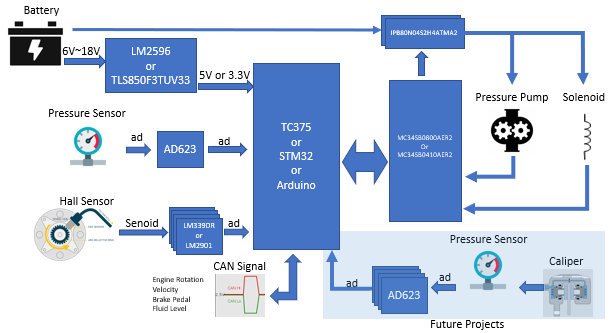
\includegraphics[width=0.92\textwidth]{figuras/arquitetura-funcional-do-sistema-de-controle-de-freio.png}%
    }{%
        \fbox{\parbox{0.92\textwidth}{\centering\vspace{8mm}
                \textbf{Figura pendente:} salvar a arquitetura funcional como\\
                \texttt{figuras/arquitetura-funcional-do-sistema-de-controle-de-freio.png}.\vspace{8mm}}}%
    }
    \Caption{\label{fig:arquitetura-funcional-do-sistema-de-controle-de-freio} Arquitetura funcional do sistema de controle proposto, destacando a integração entre simulação, controle discreto e plataforma experimental.}
\end{figure}

\section{Limita\c{c}\~oes e trabalhos futuros}
\label{sec:resultados-trabalhos-futuros}
Os resultados apresentados demonstram viabilidade em simulação e maturidade do arcabouço de implementação, mas também delimitam claramente o que ainda precisa ser validado em ambiente físico. Como continuidade direta deste trabalho, destacam-se:
\begin{itemize}
    \item implementação embarcada do controle discreto no microcontrolador (incluindo verificação de tempo de execução e temporização do laço de controle em passo fixo);
    \item integração completa do \textit{driver} de válvulas e verificação elétrica/funcional do acionamento dos atuadores;
    \item validação em bancada com o conjunto de freio, com instrumentação mínima (pressão e, quando aplicável, velocidade) para comparação com os sinais esperados em simulação;
    \item ampliar as análises de robustez para incluir ruídos (sensores, quantização), atrasos e cenários operacionais adicionais, bem como consolidar a validação experimental em bancada/HIL.
\end{itemize}

% !TeX root = ../documento.tex
\chapter{Conclusões}
\label{chap:conclusoes}

Este projeto apresenta o desenvolvimento e a validação, em ambiente de simulação, de uma metodologia de controle digital aplicada ao \textbf{regulador de pressão hidráulica} de um módulo de frenagem eletro-hidráulico (unidade ABS/ESC), com motivação em funções ADAS de controle longitudinal (por exemplo, ACC/AEB). O trabalho abrange desde a modelagem do subsistema hidráulico, passando pela implementação de estratégias de controle e estimação de estados, até a análise de desempenho por meio de simulações em MATLAB/Simulink.

Este estudo pode oferecer contribuições à comunidade acadêmica, especialmente na transposição de conceitos teóricos de controle para um contexto aplicado, com ênfase na viabilidade de implementação em hardware automotivo. 

Já a modelagem do subsistema hidráulico, baseada em equações diferenciais não lineares e posteriormente linearizada, permite a aplicação de técnicas em espaço de estados, como controle LQ em tempo discreto com integrador (LQI) e observador de Luenberger.

A arquitetura proposta demonstrou, em simulação, a capacidade de rastrear uma referência de pressão hidráulica por roda. Nesta dissertação, a referência é tratada como um sinal externo ao regulador (potencialmente oriundo de um controlador longitudinal), o que permite isolar e discutir de forma objetiva a dinâmica e as limitações do atuador hidráulico.

A cadeia conceitual de geração de referência (por exemplo, a partir de um controlador longitudinal), mapeamento para pressão, controlador LQI, observador e planta hidráulica permitiu avaliar, em simulação, tanto o seguimento de referência quanto a influência de saturações e de efeitos não lineares do modelo (por exemplo, dependência com $\Delta P$ nas leis de vazão). Quando aplicável, a análise também considera ruído de medição e variações paramétricas nos ensaios descritos.

Como síntese das principais contribuições (Seção~\ref{sec:introducao-contribuicoes}), este trabalho:
\begin{itemize}
	\item consolidou um modelo hidráulico não linear concentrado (2P) com parametrização compatível com faixas típicas de pressão e com validação qualitativa em malha aberta;
	\item apresentou um fluxo de projeto em tempo discreto para seguimento de pressão (linearização local, discretização e síntese LQI), explicitando saturações e o tratamento de \textit{windup};
	\item incorporou estimação de estados via observador de Luenberger discreto, buscando compatibilidade com instrumentação limitada;
	\item organizou a validação por simulação com \textit{scripts} e métricas, reforçando rastreabilidade entre hipótese, procedimento e evidência.
\end{itemize}

Além da validação em simulação, foi desenvolvido um protótipo de placa eletrônica como suporte à futura migração do controlador para execução embarcada e integração com um conjunto físico de frenagem.

No entanto, é importante destacar que todas as validações foram realizadas exclusivamente em ambiente simulado. Não houve, no escopo deste trabalho até a sua apresentação, a implementação prática do controle digital no microcontrolador AURIX TC375 ou em qualquer outro hardware embarcado.

A escolha do AURIX TC375 foi motivada por suas características técnicas e aderência a requisitos de segurança funcional automotiva, mas a aplicação efetiva do controle digital neste microcontrolador permanece como uma etapa futura. Assim, as conclusões aqui apresentadas devem ser interpretadas à luz das limitações do ambiente de simulação e da ausência de validação do controlador em malha fechada com atuadores/sensores reais do conjunto de freio.

Em síntese, este projeto estabelece uma base conceitual e metodológica para o desenvolvimento de sistemas de frenagem inteligentes, alinhados às tendências de direção autônoma e veículos conectados. Os resultados obtidos sugerem que é possível, ao menos em simulação, projetar e validar um regulador digital de pressão compatível com a integração a funções ADAS longitudinais. Contudo, etapas adicionais de validação prática e aprimoramento (implementação embarcada, temporização, instrumentação e ensaios em bancada) são necessárias para aplicações industriais e para consolidar a transferência tecnológica ao ambiente automotivo real.


%Elementos pós-textuais    
\bibliography{elementos-pos-textuais/referencias}
%\imprimirglossario
\imprimirapendices
\input{elementos-pos-textuais/apendices/apendice}

%% Adicione aqui os apendices do seu trabalho
%% \input{elementos-pos-textuais/apendices/historico-de-mudancas}
%% \input{elementos-pos-textuais/apendices/lorem-ipsum}
%% \input{elementos-pos-textuais/apendices/termo-de-fiel-depositario}
\imprimiranexos
%% 	Adicione aqui os anexos do seu trabalho
%% 	\input{elementos-pos-textuais/anexos/exemplo-de-anexo}
%% 	% !TeX root = ../../documento.tex
\anexo{Dinâmica das classes sociais}
\label{an:dinamica-das-classes-sociais}

\lipsum[14]
\index{AAA}
%% \imprimirindice

\end{document}
